\documentclass[openany]{ib-tesis}

%-----------------------------------------------------------------------------%
%------------------Información de Portada-------------------------------------%
%-----------------------------------------------------------------------------%
\titulo{\texorpdfstring{REPRESENTACIONES DEL\\COMPORTAMIENTO ANIMAL EN UNA\\TAREA DE APRENDIZAJE MOTOR}{REPRESENTACIONES DEL COMPORTAMIENTO ANIMAL EN UNA TAREA DE APRENDIZAJE MOTOR}}
\title{\texorpdfstring{REPRESENTATIONS OF\\ANIMAL BEHAVIOR IN A\\MOTOR SKILL LEARNING TASK}{REPRESENTATIONS OF ANIMAL BEHAVIOR IN A MOTOR SKILL LEARNING TASK}}
\orientacion{Orientación: Física en Medicina y Biología}
\autor{\textbf{Álvaro Concha}}
\director{\textbf{Dra. Soledad Espósito}}
\codirector{\textbf{Dr. Damián Hernández}}
\trabajo
{
    TESIS DE MAESTRÍA EN CIENCIAS FÍSICAS
}
\carrera
{
    MAESTRÍA EN CIENCIAS FÍSICAS
}
\grado
{
    MAESTRANDO
}
\laboratorio{\texorpdfstring{Laboratorio de Neurobiología del Movimiento\\Departamento de Física Médica\\Centro Atómico Bariloche}{Laboratorio de Neurobiología del Movimiento Departamento de Física Médica Centro Atómico Bariloche}}
\institucion{\texorpdfstring{Instituto Balseiro\\Comisión Nacional de Energía Atómica\\Universidad Nacional de Cuyo}{Instituto Balseiro Comisión Nacional de Energía Atómica Universidad Nacional de Cuyo}}
\juradoa{\textbf{Dr. Lucas Mongiat}}
\juradob{\textbf{Dr. Luciano Marpegan}}
\juradoc{\textbf{Dr. Sebastián Risau}}
\palabrasclave
{
    rotarod,
    comportamiento animal,
    UMAP,
    aprendizaje automático,
    clasificación no supervisada,
    interpretabilidad de modelos
}
\keywords
{
    rotarod,
    animal bahavior,
    UMAP,
    machine learning,
    unsupervised classification,
    model interpretability
}
\fecha{Febrero de 2022}
%-----------------------------------------------------------------------------%
%------------------Paquetes---------------------------------------------------%
%-----------------------------------------------------------------------------%

%-----Configuracion de hipervinculos (\usepackage{hyperref})-----------------------%
%\hypersetup{colorlinks=false,linkcolor=blue,citecolor=blue}

%-----Configuración de espaciado (\usepackage{setspace})---------------------------%
%\singlespacing		%para previsualizacion
%\onehalfspacing	%default
%\doublespacing		%para correccion

%-----Configuración de pagina (\usepackage{geometry})------------------------------%
%\geometry{inner=3cm,outer=2.5cm,top=3cm,bottom=3cm}	% margenes minimos
%\geometry{inner=4cm,outer=3cm,top=3.5cm,bottom=4cm}	% margenes maximos 

%-----Configuración de headers (\usepackage{fancyhdr})------------------------------%
\usepackage{fancyhdr}
\renewcommand{\chaptermark}[1]{\markboth{#1}{}}
\renewcommand{\sectionmark}[1]{\markright{#1}}
\pagestyle{fancy}
\fancyhf{}
\fancyhead[LE,RO]{\thepage}
%\fancyhead[LO]{\normalfont\nouppercase{\rightmark}}
%\fancyhead[RE]{\normalfont\nouppercase{\leftmark}}
\fancyhead[LO]{\itshape\nouppercase{\rightmark}}
\fancyhead[RE]{\itshape\nouppercase{\leftmark}}
\renewcommand{\headrulewidth}{0pt}

%-----Títulos sin separar en sílabas (no hyphenation)------------------------------%
\usepackage[raggedright]{titlesec}
\addbibresource{referencias.bib}

\def\sqrtexplained#1{%
  \begingroup
    \sbox0{$#1$}
    \def\underbrace##1_##2{##1}
    \sbox2{$#1$}
    \dimen0=\wd0 \advance\dimen0-\wd2
    \mathrlap{\sqrt{\phantom{\displaystyle#1}\kern\dimen0 }}
    \hphantom{\sqrt{\vphantom{\displaystyle#1}}}
  \endgroup
  #1}

\begin{document}

\frontmatter
\maketitle
\tableofcontents
%------------------------------------------------------------------------------%
%------------------Resumen-----------------------------------------------------%
%------------------------------------------------------------------------------%
\begin{resumen}
    Los complejos repertorios comportamentales exhibidos por animales pueden ser descritos, con diferentes grados de detalle, como combinaciones de un conjunto finito de movimientos estereotípicos o de estados biofísicos.
    Estas respuestas biofísicas son flexibles, ya que diferentes secuencias de comportamientos pueden usarse para resolver tareas similares, y también son adaptables a cambios en el entorno por medio de mecanismos de aprendizaje.
    Dada esta flexibilidad y adaptabilidad, traducir comportamientos animales complejos a características cuantificables o a categorías bien definidas es una tarea difícil.
    Por un lado, la clasificación manual de comportamientos puede consumir mucho tiempo, requerir la definición de categorías \textit{a priori}, y puede no ser reproducible entre evaluaciones.
    Por otro lado, las categorías comportamentales creadas heurísticamente (por ejemplo, caminar, correr o saltar) suelen ignorar información inherente sobre la variabilidad intra- e inter-animal, típica de los comportamientos no restringidos en entornos naturales.

    Por lo tanto, en este trabajo analizamos diferentes enfoques para cuantificar y evaluar el comportamiento de ratones durante la ejecución de una tarea de aprendizaje motor (rotarod con aceleración). En particular, aplicamos técnicas de aprendizaje automático no supervisado para la clasificación de comportamientos (mapas UMAP con segmentación \textit{watershed}).
    Primeramente, propusimos métricas de rendimiento, alternativas a la latencia a caer, para mostrar diferentes niveles de aptitud física y de aprendizaje de la tarea entre los ratones.
    Luego, usamos mapas UMAP para producir dos posibles representaciones del comportamiento de los ratones, en un espacio latente de dimensión baja.
    Una representación fue construida usando espectros de frecuencia \textit{wavelet} de partes del cuerpo de los ratones y la otra usando características extraídas de sus pasos y poses.
    Finalmente, agrupamos los comportamientos observados en categorías (\textit{labels}), realizando una segmentación \textit{watershed} sobre los mapas, y caracterizamos estos comportamientos.
    De esta manera, dilucidamos la estructura subyacente y la dinámica del comportamiento, mejorando nuestro entendimiento acerca de la ejecución y el aprendizaje de esta tarea. Los comportamientos encontrados separan a los ratones en grupos de rendimiento, y la manera en que estos comportamientos son utilizados se consolida durante el entrenamiento.
\end{resumen}
%------------------------------------------------------------------------------%
%------------------------------------------------------------------------------%
%------------------Abstract----------------------------------------------------%
%------------------------------------------------------------------------------%
\begin{abstract}
A fundamental assumption in behavioral neuroscience is that animal activity, while performing defined tasks, can be vastly described by a finite set of stereotyped behaviors. Information about animal behavior can then be correlated with simultaneous recordings of neural activity allowing us to understand how the brain encodes particular behaviors, what are the underlying neural circuits and how these circuits are modified during motor learning  \cite{esposito_defensive,levy_representation}.

However, classifying different types of movements can be a complex endeavor. On the one hand,  the extent of animal activity recordings may be too large to be manually classified and such classification may not be reproducible between subjects. On the other, heuristically created categories (e.g., walking, running, jumping) tend to ignore inherent information regarding intra- and inter-animal variability frequently found in unrestrained behavior \cite{berman_mapping}.

Therefore, in this work we used unsupervised machine learning techniques to classify different types of behaviors exhibited by expert mice performing a motor skill task. In particular, we used the t-SNE algorithm to classify animal behavior from a dataset containing information about the position of the mouse and their body parts while walking on a rotating cylinder at increasing speeds (accelerating rotarod task) \cite{berman_mapping,vdm_tsne,esposito_rotarod}.

By applying this algorithm, we were able to classify behavior into 9 individual classes that correspond to specific poses of the mouse while performing the accelerating rotarod task. These poses were found to be representative of the individual mice analyzed  ($N_{\mathrm{ratones}}=3$) and capture common aspects in their movements. In addition, we studied the dynamics of transitions between poses and their dependence with the rotarod speed. This analysis showed that at faster rotarod speed animals change their motor strategy by selecting a type of locomotion characterized by hindlimb alternation.

Finally, this pose classification was used to study potential correlations with neural activity patterns in the mesencephalic locomotor region (MLR) and we found the existence of individual neurons whose activity is modulated by the occurrence of pose transition events. Altogether, this work demonstrates the benefit of the use of unsupervised strategies for the detailed study of animal behavior and its utility in the study of neural circuit function.
\end{abstract}
%------------------------------------------------------------------------------%

\mainmatter
\chapter*{Introducción}\label{cha:introduccion}
\addcontentsline{toc}{chapter}{Introducción}

\section{Motivación}\label{sec:motivacion}

Espero que este trabajo sirva para documentar el \textit{pipeline} de procesamiento de datos.

\section{Objetivos}\label{sec:motivacion}

Esperamos que este trabajo sirva como documentación del \textit{pipeline} de procesamiento de datos, refinado luego de un año de ajustes durante el transcurso de la maestría.

Más importante aún para los intereses del laboratorio, esperamos que estas herramientas de procesamiento puedan no solamente generalizarse a nuevos experimentos o modelos de comportamiento animal, sino también brindar claridad sobre los resultados.

Un problema común en las aplicaciones que involucran el análisis de grandes volúmenes de datos es su difícil interpretabilidad. Por ejemplo, los modelos de aprendizaje automático basados en redes neuronales profundas pueden generar predicciones muy precisas, sin embargo suele ser difícil interpretar el funcionamiento del modelo [cita requerida]. De manera análoga, los mapeos no lineales son una herramienta popularizada recientemente en diversos ámbitos, desde el análisis de secuenciamiento de células individuales en bioinformática, pasando por el estudio de similaridad de textos en el análisis de lenguaje de natural, hasta sistemas de recomendación de productos usados en la industria de la información [citas requeridas].

En este sentido, la etología, ciencia que estudia el comportamiento animal, no es una excepción. Especialmente cuando abundan los registros de video de comportamiento animal, gracias al fácil acceso a cámaras digitales y su versatilidad para ser incluidas en la mayoría de los protocolos experimentales existentes. En simultáneo, la aparición de herramientas de \textit{software} para el trackeo de movimientos sin marcadores físicos, abrieron la puerta a una cantidad impensada de datos crudos. Es en este contexto de abundancia de información y escasez de métricas comportamentales detalladas, exhaustivas y cuantitativas que entran en juego los mapeos no lineales.

Aquí es donde podría entrar el rotarod y la latencia a caer

Clásicamente

Mencionar \textit{feature discovery} -> behavior labels from UMAP segmentation

Mencionar de nuevo (probablemente lo hice en la tesis) la necesidad de equiparar la cuantificación del comportamiento animal, con el aumento en la precisión y la mejora en los registros de actividad neuronal.

Además, con este enfoque, estoy analizando la biomecánica del movimiento de los ratones en la tarea rotarod. Lo cual es valioso.

Estoy "retrocediendo pasos" y "descuartizando" la caja negra del mapeo UMAP y los behavior labels. El primer paso atrás es sintetizar las frecuencias promedio de diferentes grupos de ángulos de marcadores corporales. El segundo paso atrás es calcular las diferencias de fase entre pares de ángulos de marcadores corporales.

Podría agregar otras métricas, como la volatilidad (std en una ventana móvil) de los espectros de frecuencia y de los ángulos.

Estos son los features sintetizados o interpretados. Y funcionan bastante bien con la perspectiva de label sequences averaging.

Por otro lado, puedo usar directamente los features del PCA, espectros de frecuencias y ángulos, para intentar ver qué es lo que significa cada behavior label. Esto funciona mejor con la perspectiva de label time series.

En ambas perspectivas, la idea es entrenar un árbol de decisión, que nos diga qué parte de los features decide cada label, y la importancia de cada label en esta clasificación de comportamientos.

En cuanto a descartar label sequences con duración menor a 30 frames: tiene ciertas ventajas.
Por un lado, usar label sequences de mayor duración me ayuda a obtener promedios y correlaciones mejor definidas (más número de muestras por ocurrencia de label).
Por otro lado, según el supuesto de estereotipia, un comportamiento x sigue siendo un comportamiento x, no importa si su realización dura 5 o 200 frames.
Así que para caracterizar el comportamiento, puedo concentrarme en las ocurrencias de mayor duración, para facilitar la interpretación y la estimación/cálculo de las métricas que elegí para hacerlo.

Dado que estoy elevando el espectro de frecuencias wavelet al cuardrado, lo que estoy calculando power spectral centroid, solamente que haciendo un promedio geométrico porque trabajo con canales de frecuencia de varios órdenes de magnitud diferentes (de 0.5 Hz a 50 Hz, son tres órdenes de magnitud comprendidos).

%https://dsp.stackexchange.com/questions/38643/how-to-calculate-the-mean-center-frequency-of-the-spectrum

Marcapasos aleatorio (Random Pacemaker Model)

Agregar frase como subtítutlo de esta sección

"All models are wrong, but some are useful" - George Box.

Filtros:
Median filter to denoise positions and likelihoods before Kalman
Kalman filter to reconstruct low likelihood tracking (try to correct occlusions and non-confident (low likelihood) marker swithings)
Quantile filter to correct Kalman drift and confident (high likelihood) marker switching
Finally, a trimmed mean filter, with a small window, to smooth and denoise the signal a little bit.


En etología, la ciencia que estudia el comportamiento, el supuesto de estereotipia consiste en que los comportamientos exhibidos por un animal pueden ser descompuestos en elementos discretos y reproducibles. Estos comportamientos elementales se suponen constantes a lo largo del tiempo y consistentes entre diferentes individuos y, en algunos casos, entre diferentes especies. Estos conjuntos discretos de comportamientos podrían emerger a partir de diferentes mecanismos, por ejemplo, la existencia de límites mecánicos para el control de la marcha y otros movimientos, la formación de hábitos, o la presión selectiva para ejecutar acciones robustas u óptimas en un determinado entorno. Estos mecanismos limitarían el repertorio de movimientos del animal a pesar de su potencial capacidad de moverse de infinitas maneras, restringidos en principio únicamente por los límites biomecánicos de su morfología \cite{berman_mapping,lehner_stereotipy}.

\begin{figure}[h!]
    \centering
    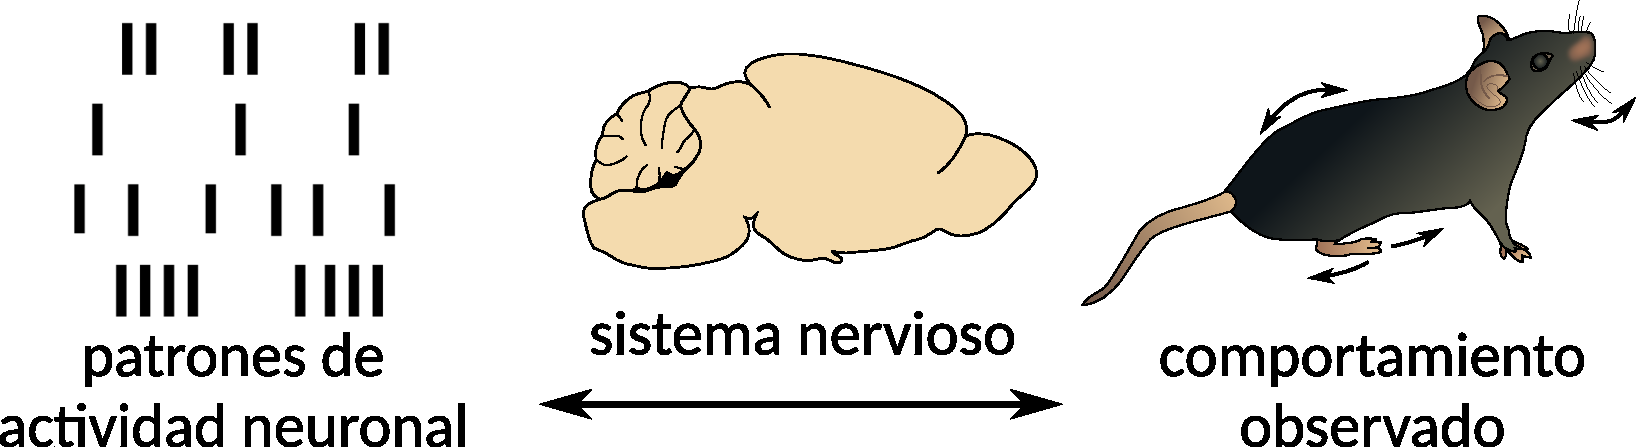
\includegraphics[width=0.6\linewidth]{figuras/introduccion/actividad_comportamiento.pdf}
    \caption{El estudio de las correlaciones entre la actividad neuronal y los comportamientos animales suscitados, puede ayudar a dilucidar el funcionamiento de diferentes regiones del sistema nervioso.}
    \label{fig:actividad_neuronal}
\end{figure}

El concepto de estereotipia tiene una gran utilidad cuando se trata de comprender cómo el cerebro controla dichos movimientos.
En este caso, la información resultante de la cuantificación del comportamiento es de fundamental importancia para su correlación con registros simultáneos de la actividad neuronal con el fin de estudiar cómo el cerebro codifica diferentes movimientos, cuáles son los circuitos neuronales subyacentes y cómo estos se modifican durante el aprendizaje de nuevas tareas motoras (Figura \ref{fig:actividad_neuronal}) \cite{esposito_defensive,levy_representation}. A pesar de su importancia, la determinación del repertorio de movimientos de un animal resulta experimentalmente complicada, debido a las dificultades que conlleva la cuantificación del comportamiento animal en términos objetivos y reproducibles.

En este trabajo nos proponemos explorar el espacio de comportamientos a los que accede un conjunto de ratones realizando una tarea de destreza motora de manera no supervisada. La tarea estudiada se denomina rotarod con aceleración, la cual consiste en entrenar ratones para que caminen sobre un cilindro que gira a velocidades crecientes, con aceleración constante. El \textit{rotarod} con aceleración es un paradigma experimental ampliamente utilizado en el estudio del aprendizaje motor dado que la \textit{performance} del animal mejora con el entrenamiento de manera dependiente de la plasticidad neuronal \cite{costa_motor_learning}. Sin embargo, el desempeño del animal en esta tarea se suele evaluar simplemente a través de la medición del tiempo de permanencia en el cilindro. En este contexto nos preguntamos, ¿cuáles son los cambios en el repertorio de movimientos del animal asociados a un mejor desempeño de la tarea? 

Para contestar esta pregunta realizamos una serie de filmaciones de los animales mientras realizaban la tarea motora. Para cuantificar los movimientos, se extrajeron coordenadas bidimensionales de las posiciones de algunas partes de sus cuerpos y su evolución en el tiempo. Para ello, se utilizó \textit{DeepLabCut}, un \textit{software} \textit{open-source} de \textit{motion-tracking}, que no requiere la utilización de marcadores físicos adicionales sobre los cuerpos de los animales \cite{mathis_deeplabcut}. A partir de estas coordenadas se calcularon posiciones relativas en función del tiempo. De esta manera, se extrajo información cuantitativa de las posiciones de los ratones y de sus partes del cuerpo durante el transcurso de la tarea \textit{rotarod}.

Para dilucidar la estructura intrínseca de este conjunto de datos se utilizó el algoritmo t-SNE para la reducción de la dimensión de manera no lineal \cite{vdm_tsne}. La transformada t-SNE es también una herramienta popular para la visualización de conjuntos de datos de dimensión alta y se utiliza frecuentemente en el ámbito de la bioinformática para visualizar datos provenientes de la secuenciación del material genético de células individuales \cite{kobak_art}. Así se construyó un mapa de comportamientos en 2 dimensiones donde se proyectan cada uno de nuestros vectores de dimensión mayor que describen la posición de los ratones y de sus partes del cuerpo.

Luego, procedimos a analizar la dinámica de transiciones en este espacio de dimensión reducida producido por el algoritmo t-SNE y se identificaron \textit{clusters} de puntos que se corresponden con poses específicas adoptadas por los ratones durante la ejecución de la tarea \textit{rotarod}. Así, se utilizó de manera efectiva al algoritmo t-SNE para la clasificación no supervisada de poses animales. Esta clasificación es robusta y representativa de nuestro conjunto de ratones estudiados ($N_{\mathrm{ratones}}=3$) y tiene potencial tanto como para reimplementarse utilizando un mayor número de ratones \textit{a priori}, como también para agregar nuevas observaciones experimentales al mapa t-SNE \textit{a posteriori} \cite{kobak_art, korsunsky_harmony}. Interpretaremos entonces como comportamientos estereotipados a diferentes sucesiones de estas poses clasificadas. En particular, nos concentraremos en el estudio de transiciones de primer orden entre dos poses distintas, pero también exploraremos la dinámica de transiciones de poses a escalas de tiempo mayores.

En simultáneo, durante la ejecución de la tarea \textit{rotarod}, se registró la actividad de neuronas individuales de la región locomotora del mesencéfalo (MLR) de los ratones ya entrenados en la tarea. El MLR es una región implicada en los procesos de iniciación y de control de la velocidad de la locomoción \cite{caggiano_midbrain, roseberry_locomotor, shik_walking}. Por lo tanto, en este experimento nos preguntamos si la actividad de algunas de las neuronas presentes en esta región del cerebro estaría modulada por el movimiento del ratón en el transcurso de la tarea \textit{rotarod} \cite{skinner_mlr_rat, sherman_mlr_cat, leray_mlr_vertebrate}. Para contestar esta pregunta correlacionamos la actividad neuronal con la ocurrencia de transiciones entre poses específicas obtenidas a partir de la clasificación no supervisada del comportamiento. Este estudio nos permitió demostrar la existencia de neuronas en el MLR (alrededor de un cuarto del total de neuronas registradas) cuya actividad neuronal varía significativamente alrededor de las transiciones entre poses clasificadas. Este resultado sugiere fuertemente que el MLR no solo codificaría la iniciación y la velocidad de la locomoción sino también el tipo de movimiento seleccionado.

\thispagestyle{empty}
\chapter{Método experimental}\label{cha:metodo_experimental}

\AddToShipoutPictureBG*{\put(0,0){%
        \parbox[b][\paperheight]{\paperwidth}{%
            \vfill
            \centering
            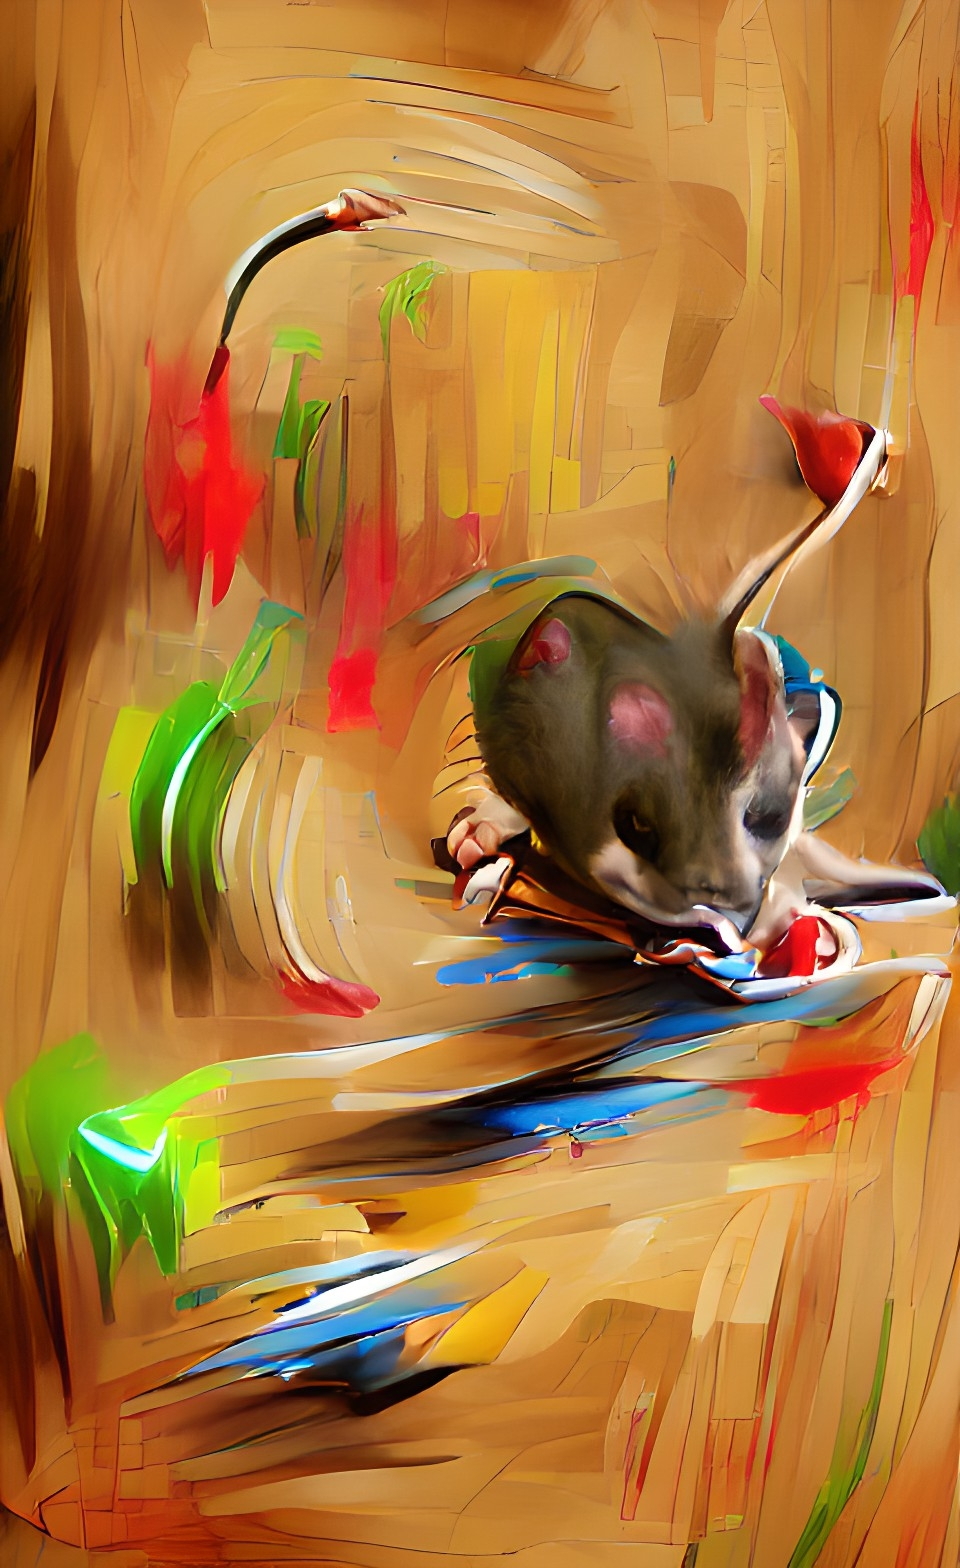
\includegraphics[width=\paperwidth,height=\paperheight,keepaspectratio]{%
                figuras/caratulas/metodo_experimental.jpg}\vfill
        }}}

\AddToShipoutPicture*{
    \begin{tikzpicture}[overlay, remember picture]
        \fill[white, opacity=0.75] (20, 24) rectangle (1, 21);
    \end{tikzpicture}}

\clearpage

Tradicionalmente, predominan dos enfoques a la hora de diseñar experimentos comportamentales en neurociencia. Por un lado, en los estudios de psicología comparada, se analiza el comportamiento como respuesta a estímulos positivos o negativos. Esta perspectiva condujo al desarrollo de trabajos donde los animales se entrenan en el laboratorio para responder a señales sensoriales, recompensas y castigos. Luego, al combinar estos métodos comportamentales con registros y manipulaciones de la actividad neuronal se logra responder preguntas fundamentales sobre cómo están codificadas las variables relacionadas a la tarea comportamental en diferentes regiones del cerebro y qué circuitos neuronales están involucrados. En general, se entrena a los animales para producir acciones relativamente simples (por ejemplo, alcanzar un \textit{pellet} o interactuar con un \textit{lick port}) fáciles de medir y de estudiar junto con patrones de actividad neuronal. Además, suelen utilizarse restricciones físicas para inmovilizar o reducir el movimiento espontáneo de los animales, tanto para facilitar los registros neuronales como para eliminar correlaciones espurias \cite{datta_computational_neuroethology}.

Por otro lado, los estudios etológicos se concentran históricamente en el comportamiento de los animales en entornos naturales \cite{tinbergen_instinct}. La hipótesis subyacente es que exponer la estructura del comportamiento, cómo está compuesto en términos de comportamientos estereotipados y cómo está organizado para responder a estímulos ecológicamente relevantes (es decir, vitales para la supervivencia de la especie y para la adaptación a un entorno) brinda información valiosa sobre cómo el cerebro genera estos comportamientos. Sin embargo, tradicionalmente la etología se concentró en observar el comportamiento animal sin intervenir ni registrar la actividad neuronal. Por lo tanto, explorar la actividad neuronal junto con comportamientos complejos en contextos naturales (por ejemplo, la exploración de nuevos entornos, la obtención de alimento, la búsqueda de refugio o el cortejo, los cuales son comportamientos de iniciativa propia y desarrollados sin mayores restricciones físicas experimentales) tiene el potencial de revelar cómo el cerebro lleva a cabo tareas evolutivamente más importantes. Finalmente, la etología ha mostrado que muchos comportamientos naturales pueden representarse como secuencias de componentes categorizables. En principio, esto permite analizar las relaciones entre las diferentes categorías comportamentales y la actividad neuronal, a lo largo de múltiples escalas temporales y diferentes niveles de detalle en la descripción comportamental \cite{datta_computational_neuroethology, anderson_toward_a_science}.

\clearpage

\begin{figure}[htbp]
    \centering
    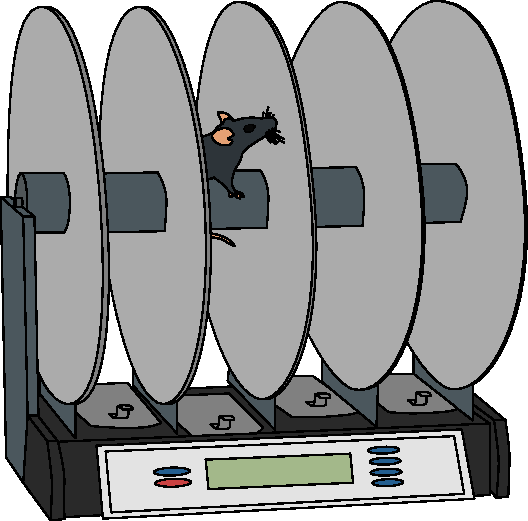
\includegraphics[width=0.5\linewidth]{figuras/capitulo1/rotarod.pdf}
    \caption{\textbf{Aparato rotarod.} El aparato consiste en una varilla rotatoria, compartimentalizada en varias secciones. Un ratón se coloca en una de estas secciones y debe caminar sobre el cilindro que gira a velocidades crecientes.}
    \label{fig:capitulo1_rotarod}
\end{figure}

\section{Protocolo rotarod con aceleración}\label{sec:protocolo}

En este trabajo estudiamos el comportamiento de ratones durante el aprendizaje de la tarea rotarod con aceleración (\autoref{fig:capitulo1_rotarod}). El aparato rotarod está compuesto por una varilla rotatoria, elevada por medio de soportes laterales (\autoref{fig:capitulo1_rotarod}). La elevación de la varilla sirve para desalentar que los ratones salten voluntariamente desde la varilla hacia la mesada, interrumpiendo el correcto desarrollo de la prueba \cite{mouse_tests}. La varilla está compartimentalizada en varias secciones, en principio para poder evaluar a múltiples ratones en paralelo. En la práctica, sin embargo, cada prueba se lleva a cabo con un único ratón por vez sobre el cilindro. Esto se debe a que la presencia de múltiples ratones sobre el cilindro influye en sus comportamientos individuales. El cilindro tiene un diámetro de 3 cm y cada compartimiento del rotarod tiene un ancho de 5.7 cm.

El protocolo de entrenamiento de los ratones consiste en 2 etapas:
\begin{itemize}
    \item La primera etapa abarca 1 o 2 días de habituación antes de dar inicio a la etapa de entrenamiento propiamente dicha. Antes de iniciar las sesiones de entrenamiento (pruebas), los animales son habituados al experimentador y al ambiente del experimento (es decir, a la sala donde se encuentra el aparato rotarod). En esta etapa, los ratones son trasladados a la sala de experimentación y expuestos al rotarod, fuera de funcionamiento, durante un intervalo de tiempo de entre 10 a 15 minutos.

    \item La segunda etapa corresponde al entrenamiento \textit{per se} y es la etapa que se registra en video para posterior análisis. Cada uno de los 10 ratones estudiados se entrena durante 5 días consecutivos. Cada día de entrenamiento consiste en 5 pruebas sucesivas de rotarod, separadas entre sí por 5 minutos de descanso. Las pruebas se llevan a cabo de manera regular durante la mañana, para reducir factores que confundan con el ritmo circadiano de un mismo ratón. En cada prueba el animal es colocado sobre el cilindro rotarod, que gira a velocidades crecientes con aceleración constante, desde 5 rpm hasta 50 rpm en 5 minutos. La prueba termina cuando transcurren un máximo de 5 minutos o cuando el ratón se cae del cilindro. El tiempo transcurrido hasta el fin de la prueba se denomina latencia a caer, y es una métrica clásica para evaluar rendimiento y aprendizaje motor.
\end{itemize}

Originalmente, al aparato rotarod fue diseñado para realizar mediciones automatizadas de déficit neurológico e impedimento motor en roedores, y es actualmente uno de los métodos más comunes para evaluar rendimiento y aprendizaje motor \cite{dunham_rotarod, mouse_tests}. En cuanto a su complejidad, los comportamientos exhibidos en esta tarea están entre los comportamientos sencillos de los experimentos altamente restringidos de la psicología comparada y los comportamientos complejos observados en entornos naturales de la etología. Específicamente, en la tarea rotarod existen restricciones sobre el desplazamiento y la velocidad del ratón, ya que debe caminar sobre un cilindro de dimensiones finitas a una velocidad controlada experimentalmente. Sin embargo, la manera en que el ratón se adapta a estas restricciones biomecánicas es no trivial y varía entre individuos y a lo largo del entrenamiento. Por este motivo, consideramos a la tarea rotarod como ecológicamente relevante, respecto del aprendizaje motor. Principalmente porque expone la manera en que el ratón se adapta a un nuevo entorno y muestra los cambios que sufre su estrategia comportamental para resolver la tarea, siendo esta adaptabilidad a nuevos entornos una habilidad crucial para la supervivencia.

\section{Registros en video}\label{sec:video}

Cada una de las pruebas realizadas se registra en video usando un arreglo de 2 cámaras digitales (\autoref{fig:capitulo1_camaras}). Cada cámara tiene una frecuencia de muestreo de 100 Hz (resolución temporal de 10 ms), capturando fotogramas de 480 px de alto por 640 px de ancho. Por su parte, la cámara frontal captura los movimientos de la cabeza, de las patas delanteras y de parte del lomo del ratón, mientras que la cámara trasera filma los movimientos caudales, de las patas traseras y del lomo del ratón.

\begin{figure}[htbp]
    \centering
    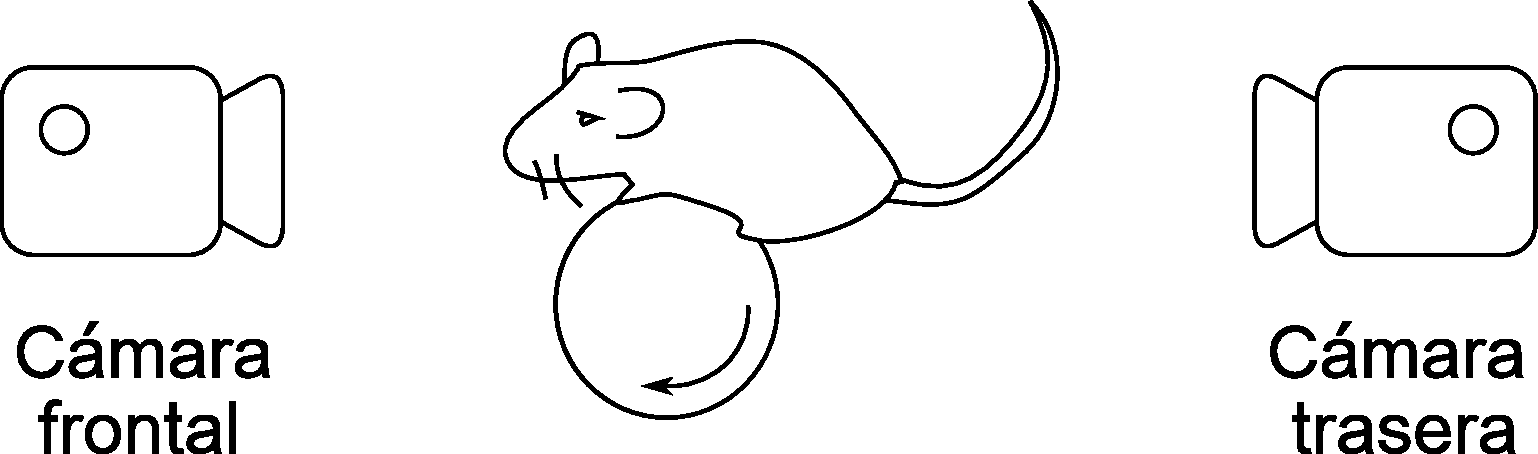
\includegraphics[width=0.55\linewidth]{figuras/capitulo1/camaras.pdf}
    \caption{\textbf{Esquema de cámaras utilizadas.} Cámara frontal, aparato rotarod y cámara trasera.}
    \label{fig:capitulo1_camaras}
\end{figure}
\chapter{Extracción de características}\label{cha:extraccion_caracteristicas}

\AddToShipoutPictureBG*{\put(0,0){%
        \parbox[b][\paperheight]{\paperwidth}{%
            \vfill
            \centering
            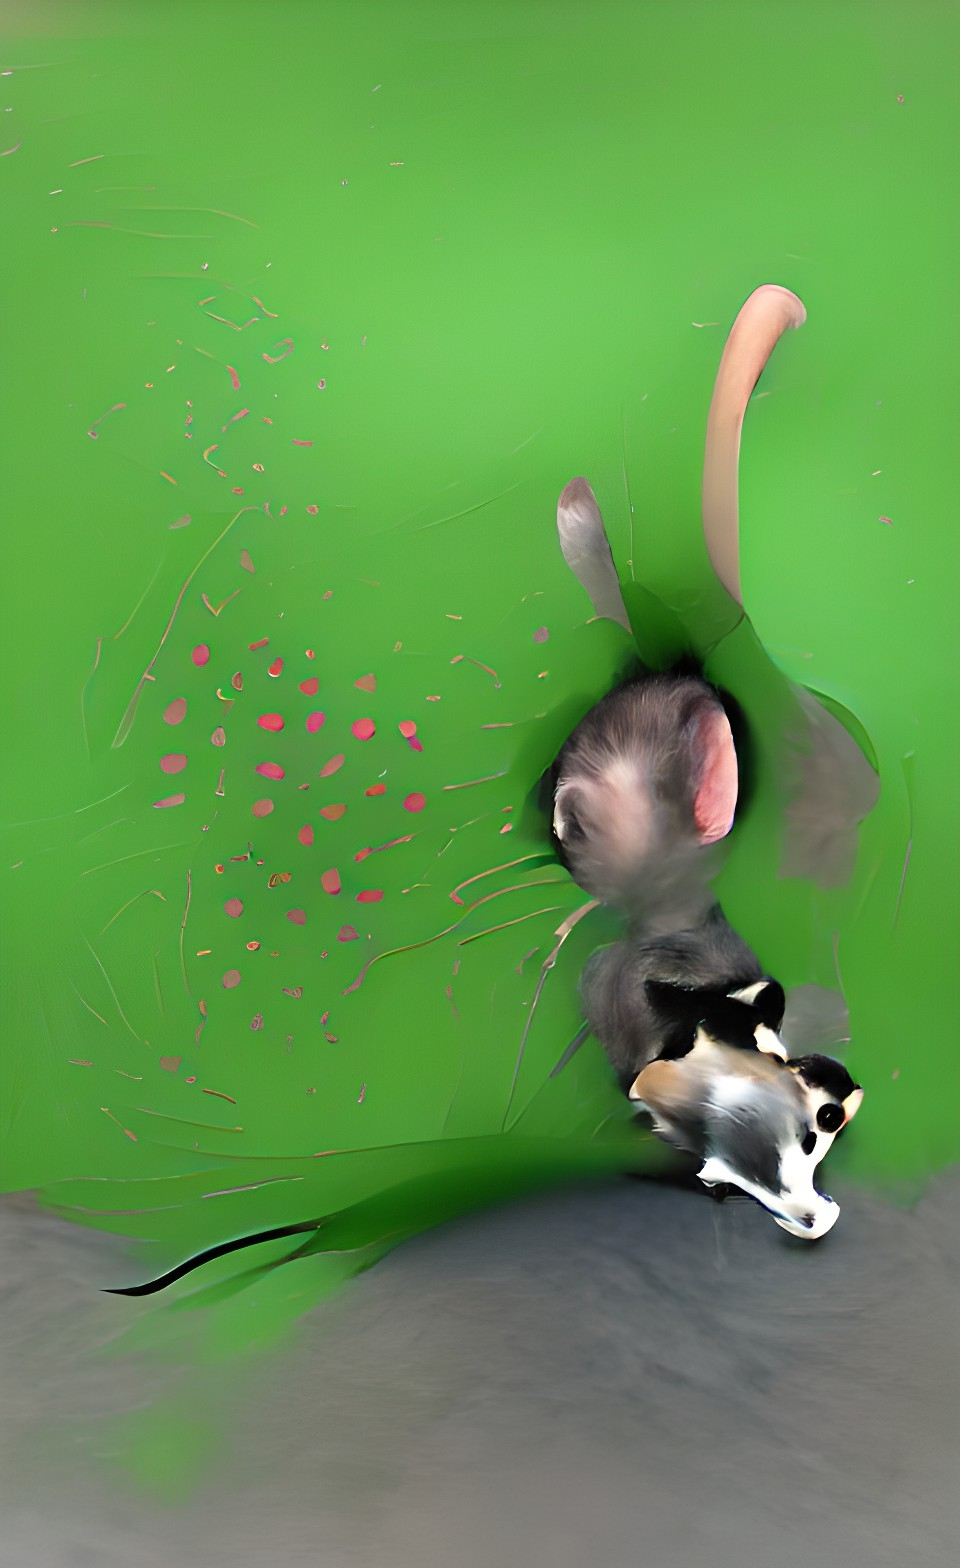
\includegraphics[width=\paperwidth,height=\paperheight,keepaspectratio]{%
                figuras/caratulas/extraccion_de_caracteristicas.jpg}\vfill
        }}}

\AddToShipoutPicture*{
    \begin{tikzpicture}[overlay, remember picture]
        \fill[white, opacity=0.75] (20, 24) rectangle (1, 21);
    \end{tikzpicture}}

\clearpage

El comportamiento animal es inherentemente dinámico y evoluciona en el tiempo. Para capturar la estructura temporal del comportamiento es necesario medir variables biofísicas de los animales a lo largo del tiempo. Estas son diversas características que están asociadas a las partes del cuerpo, las poses y la dinámica de los movimientos de los animales estudiados. El objetivo último del proceso de extracción de características es encontrar conjuntos de variables adecuados que mejor describan los tipos de comportamientos que queremos estudiar (esto es, que mejor separen en categorías a los patrones de movimiento o a los estados biofísicos de los animales). Debido a su fácil incorporación en los experimentos comportamentales, en este trabajo consideramos únicamente características que se extraen de los registros de video de los ratones, durante la ejecución de la tarea rotarod. Sin embargo, existen otros tipos de señales biofísicas que se utilizan para describir el comportamiento, como por ejemplo los registros de audio de vocalizaciones de aves y otros animales, como ratones, murciélagos, ballenas o primates \cite{miranda_mouse_vocals, sainburg_birdsong_umap}.

\section{Captura de movimiento}\label{sec:captura_movimiento}

Recientemente, una de las aplicaciones de aprendizaje automático que más impactó en la neurociencia del comportamiento es la captura de movimiento sin marcadores \cite{datta_computational_neuroethology}. Los avances en captura de movimiento permiten medir las posiciones de las partes del cuerpo de los animales, y de otros puntos de interés, sin la necesidad de colocar marcadores físicos adicionales ni de utilizar cámaras especializadas.

En este trabajo, utilizamos DeepLabCut, una herramienta de código abierto para estimar las posiciones de marcadores digitales definidos por el usuario (\autoref{fig:capitulo2_posiciones}) \cite{mathis_deeplabcut}. DeepLabCut utiliza redes neuronales artificiales profundas, que se entrenan con pocos fotogramas de video (típicamente, entre 50 y 200 fotogramas) para adecuarlas a las condiciones experimentales particulares del experimento, alcanzado una precisión equivalente a la humana. Con esta herramienta, se procesaron más de 10 millones de fotogramas (más de 30 hs de video), provenientes de las filmaciones de 2 cámaras (frontal y trasera) que registraron un total de 250 pruebas rotarod, realizadas por 10 ratones. Cada ratón realizó 5 pruebas por día, durante 5 días de entrenamiento, siendo la duración promedio ($\pm$ desviación estándar) de una prueba ($220 \pm 50$) s, lo cual equivale a 22\,000 fotogramas a una frecuencia de muestreo de 100 Hz.

\begin{figure}[htbp]
    \centering
    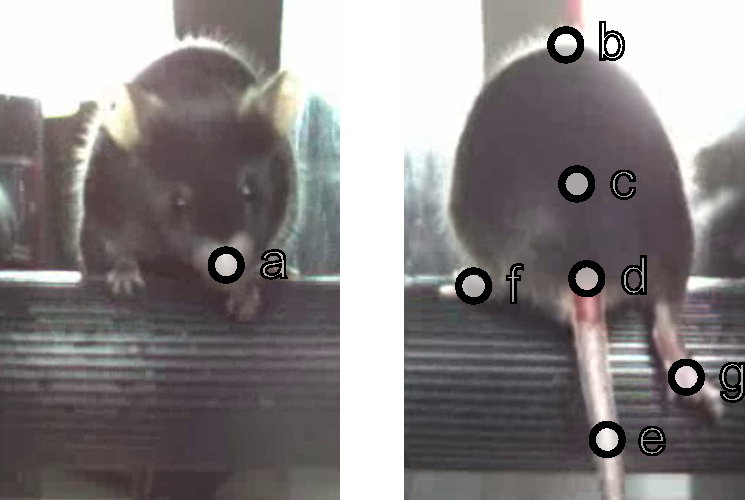
\includegraphics[width=0.65\linewidth]{figuras/capitulo2/captura_movimiento.pdf}
    \caption{\textbf{Captura de movimiento.} Marcadores digitales utilizados en el seguimiento de las partes del cuerpo del ratón.
        (Izquierda) Cámara frontal. (Derecha) Cámara trasera.
        Marcadores: (a) nariz, (b) espalda, (c) centro de masa, (d) base de la cola, (e) mitad de la cola, (f) pata trasera izquierda, (g) pata trasera derecha.}
    \label{fig:capitulo2_captura_movimiento}
\end{figure}

Si bien la tecnología de captura de movimiento avanzó mucho con la introducción de las redes neuronales artificiales, las posiciones estimadas por DeepLabCut deben procesarse \textit{a posteriori} para corregir problemas en la captura de movimiento. Se aplicaron, en el siguiente orden, un filtro de mediana, una transformación de perspectiva, un filtro de Kalman, un filtro de \textit{clipping} y un filtro de \textit{trimmed mean} sobre las señales. Aprovechamos que la captura de movimiento con DeepLabCut devuelve las \textit{likelihoods} de las estimaciones de las posiciones de los marcadores y utilizamos esas \textit{likelihoods} para calcular los errores en el filtro de Kalman. La implementación en Python de estos filtros se puede encontrar en el repositorio \href{https://github.com/alvaro-concha/animal-behavior-preprocessing}{\color{blue}{animal-behavior-preprocessing}} y los parámetros utilizados se pueden consultar en el archivo de configuración \href{https://github.com/alvaro-concha/animal-behavior-preprocessing/blob/main/animal_behavior_preprocessing/config.py}{\color{blue}{\texttt{config.py}}}. Desafortunadamente, este procesamiento de las señales reduce su frecuencia de muestreo efectiva alrededor de 30 Hz. El motivo del procesamiento es corregir las posiciones de los marcadores digitales cuando se producen oclusiones totales o parciales de los mismos, reducir el \textit{switching} entre marcadores similares (por ejemplo, confusión entre los marcadores de las patas izquierda y derecha) y compatibilizar los registros de las cámaras frontal y trasera con la transformación de perspectiva, para llevar las posiciones medidas al mismo sistema de referencia.

Una vez llevadas al mismo sistema de referencia usando la transformación de perspectiva, se combinaron las capturas de movimiento de ambas cámaras. La transformación de perspectiva se computó para cada filmación tomando como referencia a las 4 esquinas visibles del cilindro rotarod en el compartimento donde se ubica el ratón. Estas 4 esquinas se llevaron a un sistema de referencia en el que forman un rectángulo de 5.7 cm de ancho por 3 cm de alto, de acuerdo a las dimensiones del aparato rotarod. Así, se obtuvieron las posiciones en el tiempo de varios marcadores, cada uno descritos por una posición horizontal y vertical (\autoref{fig:capitulo2_posiciones}). La posición de la nariz del ratón se obtuvo usando la cámara frontal y las posiciones de la espalda, centro de masa, base de la cola, mitad de la cola y patas traseras usando la cámara trasera (\autoref{fig:capitulo2_captura_movimiento}).

\clearpage

\section{Ángulos entre partes del cuerpo}\label{sec:angulos_entre_partes}

Una vez procesadas y combinadas las posiciones de los marcadores de ambas cámaras, estas se utilizan para calcular los ángulos sostenidos entre diferentes partes del cuerpo del ratón. Los ángulos entre marcadores son invariantes ante traslaciones y rotaciones rígidas y cambios de escala. Por lo tanto, trabajar con ángulos permite ignorar diferencias de tamaño entre individuos, aunque puede perderse información relacionada con la posición y la orientación del ratón y sus partes del cuerpo sobre el cilindro. Para el cálculo de los ángulos es necesario definir tripletes (i j k) con i, j, k símbolos de los marcadores, con el que se calcula el ángulo entre los vectores $\vec{\mathrm{ij}}$ y $\vec{\mathrm{jk}}$. Al conectar los tripletes con líneas se obtienen esqueletos que representan los ángulos extraídos (\autoref{fig:capitulo2_angulos_esqueleto}). Estos ángulos adoptan rangos de valores diferentes (\autoref{fig:capitulo2_angulos}), por lo que es necesario estandarizarlos para que todos tengan el mismo rango de valores. El motivo de esta estandarización es volver comparables a los ángulos que varían poco con los que varían mucho, y que estos últimos no dominen en la representación comportamental a causa de la mayor escala de su rango de valores.

\begin{figure}[htbp]
    \centering
    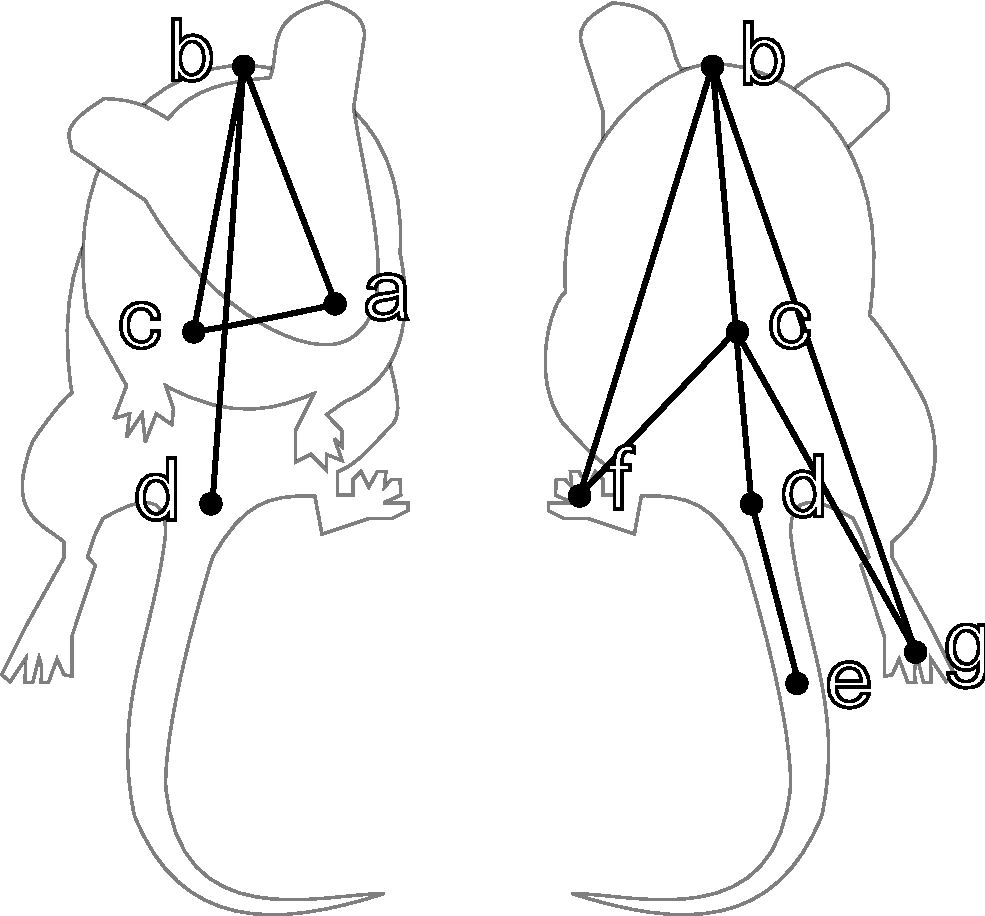
\includegraphics[width=0.5\linewidth]{figuras/capitulo2/angulos_esqueleto.pdf}
    \caption{\textbf{Ángulos de partes del cuerpo.} Esqueletos (líneas y polígonos) sobre ilustraciones de la silueta del ratón, con los que se calcularon los ángulos entre marcadores.
        (Izquierda) Frente (Derecha) Dorso.
        Marcadores: (a) nariz, (b) espalda, (c) centro de masa, (d) base de la cola, (e) mitad de la cola, (f) pata trasera izquierda, (g) pata trasera derecha.}
    \label{fig:capitulo2_angulos_esqueleto}
\end{figure}

\section{Espectros \textit{wavelet} de los ángulos}\label{sec:espectros_wavelet}

Para capturar la dinámica del movimiento de los ratones a diferentes escalas temporales simultáneamente se realiza una transformada \textit{wavelet} sobre los ángulos de las partes del cuerpo del ratón en función del tiempo. La transformada \textit{wavelet} en una convolución entre una señal (en nuestro caso, los ángulos de partes del cuerpo) y una función que depende del tiempo (el \textit{wavelet} propiamente dicho) que depende de un parámetro de escala temporal.  Al variar este parámetro de escala se exploran componentes de diferentes frecuencias presentes en la señal de interés. En particular, para tener mayor sensibilidad a la ocurrencia de intervalos de movimiento periódico, utilizamos \textit{wavelets} de tipo Morlet \cite{berman_mapping}. De esta manera, se obtuvieron las componentes de potencia espectral de las señales en 50 canales de frecuencia, distribuidos diádicamente (esto es, uniformemente en escala logarítmica) desde 0.1 Hz hasta 10 Hz (\autoref{fig:capitulo2_espectros_wavelet}). Estas componentes espectrales varían en el tiempo, al igual que las señales originales, con una resolución temporal de 10 ms. En total, al finalizar el cálculo de cada espectro \textit{wavelet}, se obtienen 50 nuevas variables por cada ángulo. Por lo tanto, pasamos de 10 ángulos entre partes del cuerpo a 500 variables que describen sus componentes espectrales. De esta manera, podemos capturar combinaciones de movimientos de diferentes partes del cuerpo del animal a distintas frecuencias.

Los espectros \textit{wavelet} son invariantes ante pequeñas traslaciones temporales (cambios de fase) en la señal, por lo que se pierde información respecto de las fases de las señales y las diferencias de fase entre las mismas. Esto significa que los espectros \textit{wavelet} pueden ignorar información sobre la sincronización entre partes del cuerpo, si es que esta información se manifiesta por medio de una diferencia de fase en el movimiento de los ángulos (\autoref{fig:capitulo4_mi_mean_wav_scaler_stp} y \autoref{fig:capitulo4_mi_pca_wav_scaler_stp}). A su vez, los espectros \textit{wavelet} de los ángulos entre partes del cuerpo heredan algunas de sus propiedades, y son también invariantes ante traslaciones y rotaciones rígidas de los marcadores y cambios de escala espaciales. Que la transformada \textit{wavelet} sea invariante ante tantas operaciones matemáticas puede parecer una desventaja, pero en ciertas situaciones es en realidad una virtud. Al ser tan robustos frente a varios tipos de perturbaciones, los espectros \textit{wavelet} de los ángulos de partes del cuerpo de animales permiten generalizar fácilmente a diferentes condiciones experimentales, e incluso, permiten que se puedan analizar diferentes especies de animales con la misma técnica, concentrándose solamente en los aspectos que tienen en común la dinámica de sus movimientos.

\section{Características de pasos}\label{sec:caracteristicas_pasos}

Una manera alternativa de extraer características comportamentales es diseñando nuestra propia ingeniería de características. Esto significa aplicar nuestro conocimiento del dominio del comportamiento animal para definir las características que nos interesen particularmente. Una ventaja de este enfoque es que podemos calcular características que sean directamente interpretables y que en pocas variables capturen información relevante del sistema. Como contrapartida, una ingeniería de características muy específica puede consumir mucho tiempo de desarrollo y puede ser difícil de generalizar a otros conjuntos de datos o dominios de problemas.

En este trabajo, definimos un conjunto de características asociadas a los pasos ejecutados por los ratones (\autoref{fig:capitulo2_caracteristicas_de_pasos}). Para ello, aprovechamos que las posiciones verticales de las patas traseras presentan máximos y mínimos locales cada vez que el ratón realiza un paso. Por lo tanto, podemos calcular derivadas de estas señales y determinar de manera relativamente sencilla los tiempos en los que el ratón da un paso. Conociendo estos instantes de tiempo, se obtienen las alturas mínima y máxima de las patas traseras en el entorno del tiempo del paso; la amplitud del paso como la diferencia entre estas alturas máxima y mínima; la velocidad del paso como el máximo local en la primera derivada de la posición vertical de la pata trasera; el desfasaje entre los pasos de ambas patas; y la frecuencia con la que el ratón da pasos con cada pata.

Una vez que tenemos calculados los eventos de ocurrencia de pasos y sus características asociadas, hacemos estadística sobre ellos. Para capturar la manera en que los eventos de pasos evolucionan en el tiempo, calculamos su promedio y desviación estándar en una ventana móvil. Esta ventana abarca 11 pasos consecutivos: lo suficientemente grande como para hacer estadística robusta, pero lo suficientemente pequeña como para capturar variaciones en la estrategia comportamental del ratón en escalas de tiempo de entre 1 s a 10 s (\autoref{fig:capitulo2_estadistica_de_pasos}).

\begin{figure}[htbp]
    \centering
    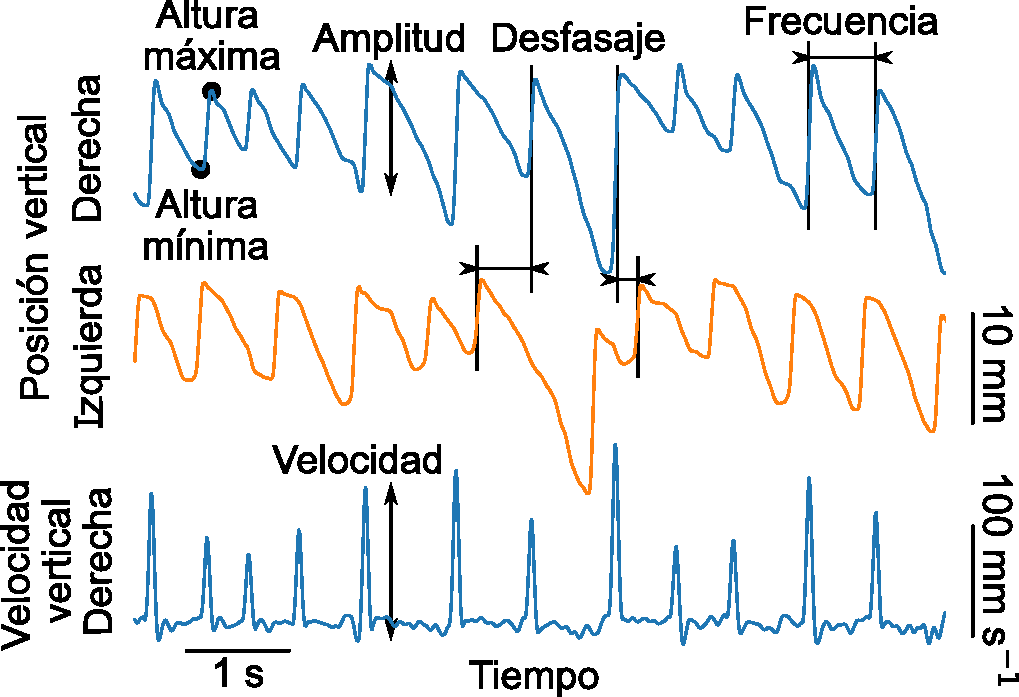
\includegraphics[width=0.65\linewidth]{figuras/capitulo2/caracteristicas_de_pasos.pdf}
    \caption{\textbf{Medición de las características de pasos.}
        Ilustración de las diferentes características asociadas a los pasos de las patas traseras.
        Este ejemplo se centra en la pata derecha.}
    \label{fig:capitulo2_caracteristicas_de_pasos}
\end{figure}

\begin{figure}[htbp]
    \centering
    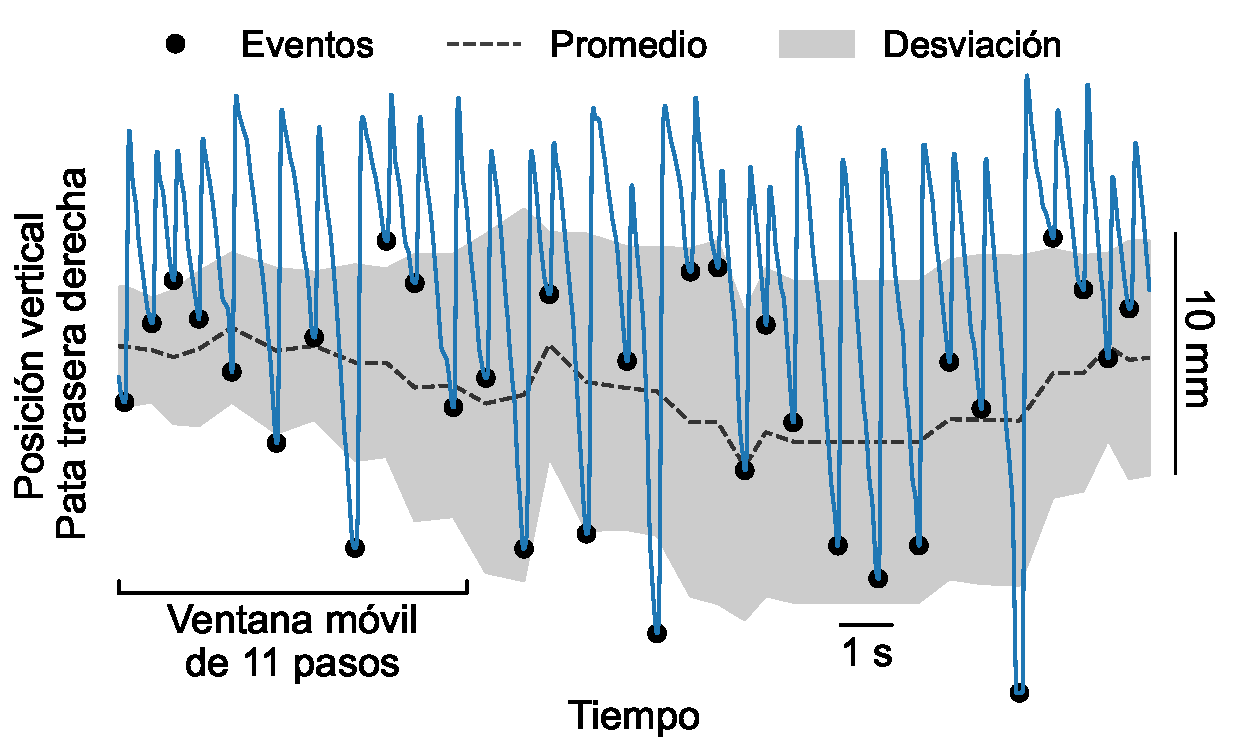
\includegraphics[width=0.8\linewidth]{figuras/capitulo2/estadistica_de_pasos.pdf}
    \caption{\textbf{Estadísticas de las características de pasos.}
        Estimación del promedio y de la desviación estándar de las características de los pasos de las patas traseras.
        Las estadísticas se calculan usando ventanas móviles de 11 pasos consecutivos, sobre las patas izquierda y derecha por separado.
        Este ejemplo se centra en la altura mínima de la pata derecha como característica.}
    \label{fig:capitulo2_estadistica_de_pasos}
\end{figure}
\chapter{Representaciones del comportamiento}\label{cha:representacion_comportamiento}

\AddToShipoutPictureBG*{\put(0,0){%
        \parbox[b][\paperheight]{\paperwidth}{%
            \vfill
            \centering
            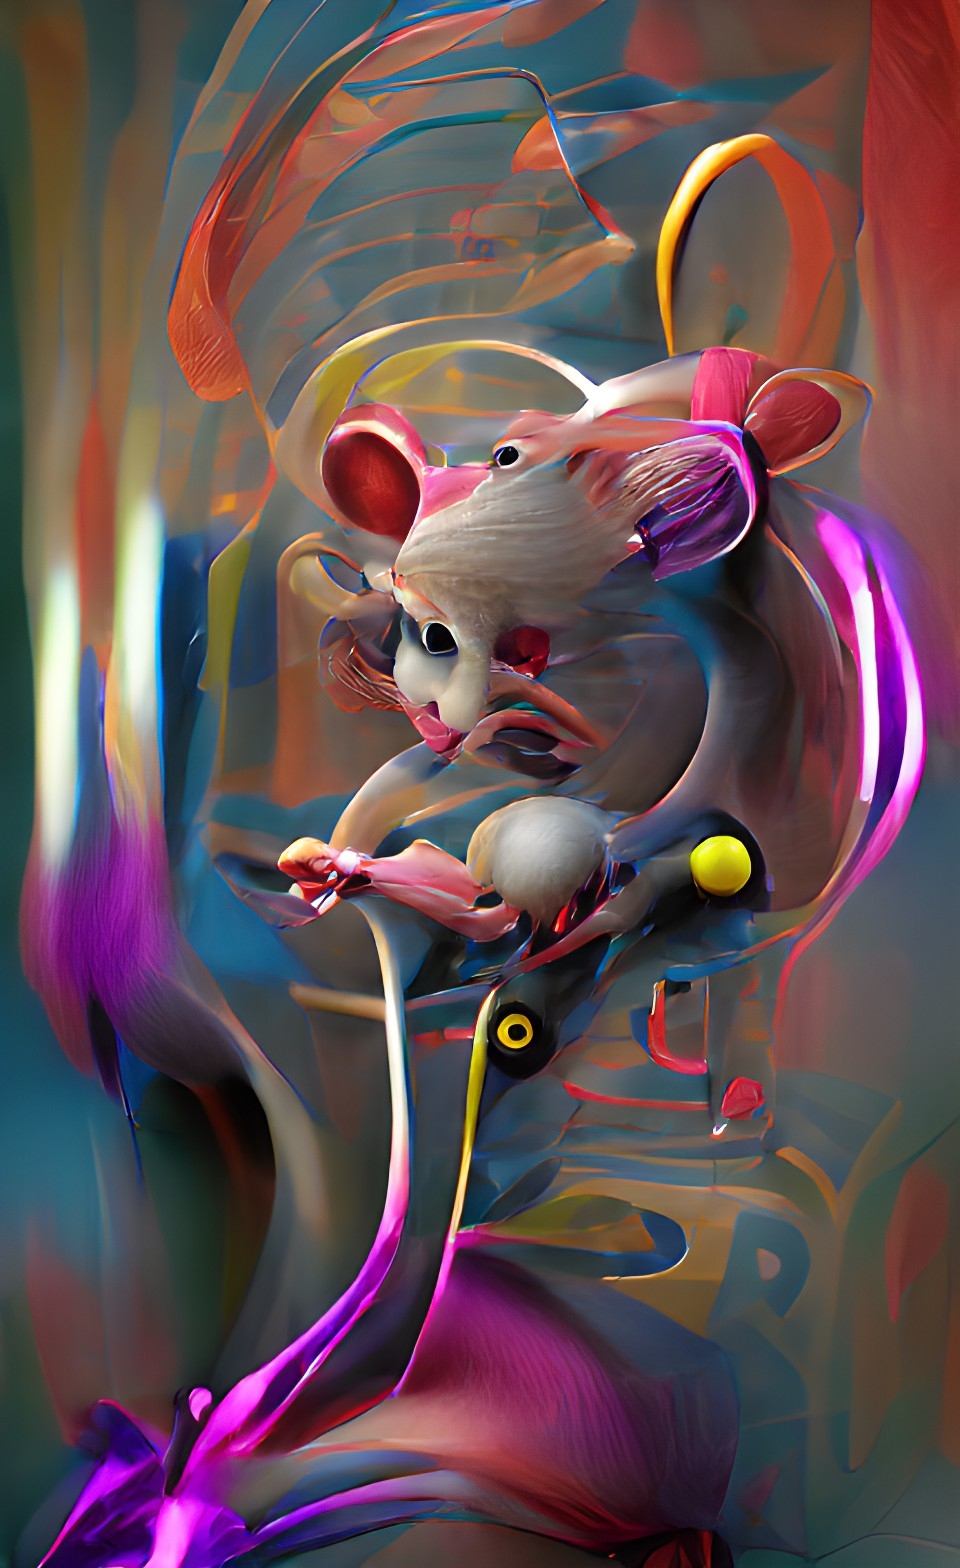
\includegraphics[width=\paperwidth,height=\paperheight,keepaspectratio]{%
                figuras/caratulas/representacion_del_comportamiento.jpg}\vfill
        }}}

\AddToShipoutPicture*{
    \begin{tikzpicture}[overlay, remember picture]
        \fill[white, opacity=0.75] (20, 24) rectangle (1, 20);
    \end{tikzpicture}}

\clearpage

\section{Niveles de descripción del comportamiento}\label{sec:niveles_descripcion_comportamiento}

Existen diferentes niveles de granularidad para describir el comportamiento animal \cite{datta_computational_neuroethology}.
Esta granularidad depende del nivel de detalle que se utilice en la caracterización anatómica, funcional y temporal del sistema. Por ejemplo, la locomoción de un animal se puede describir desde el nivel celular como contracciones y relajaciones de fibras musculares, o a grandes rasgos simplemente determinando si el animal está quieto o en movimiento.

En este sentido, nosotros utilizamos métricas que describen el comportamiento de manera global, en la escala temporal de la duración de la tarea motora (\autoref{fig:capitulo3_representacion_comportamiento}). Estas métricas son un resumen general del rendimiento y de la ejecución de una prueba, sin entrar en demasiados detalles sobre lo que sucedió a pequeña escala. Las métricas también se conocen como puntajes o \textit{scores}, pues son la principal manera de evaluar el rendimiento de una tarea realizada. A su vez, describir el comportamiento animal usando métricas, que resumen lo ocurrido en una tarea entera, permite analizar patrones de variación del comportamiento a escalas temporales más largas (por ejemplo, permite estudiar variaciones a lo largo de varias pruebas sucesivas y a lo largo de días de entrenamiento, revelando fenómenos de fatiga, aprendizaje, deterioro neurológico, entre otros).

\begin{figure}[htbp]
    \centering
    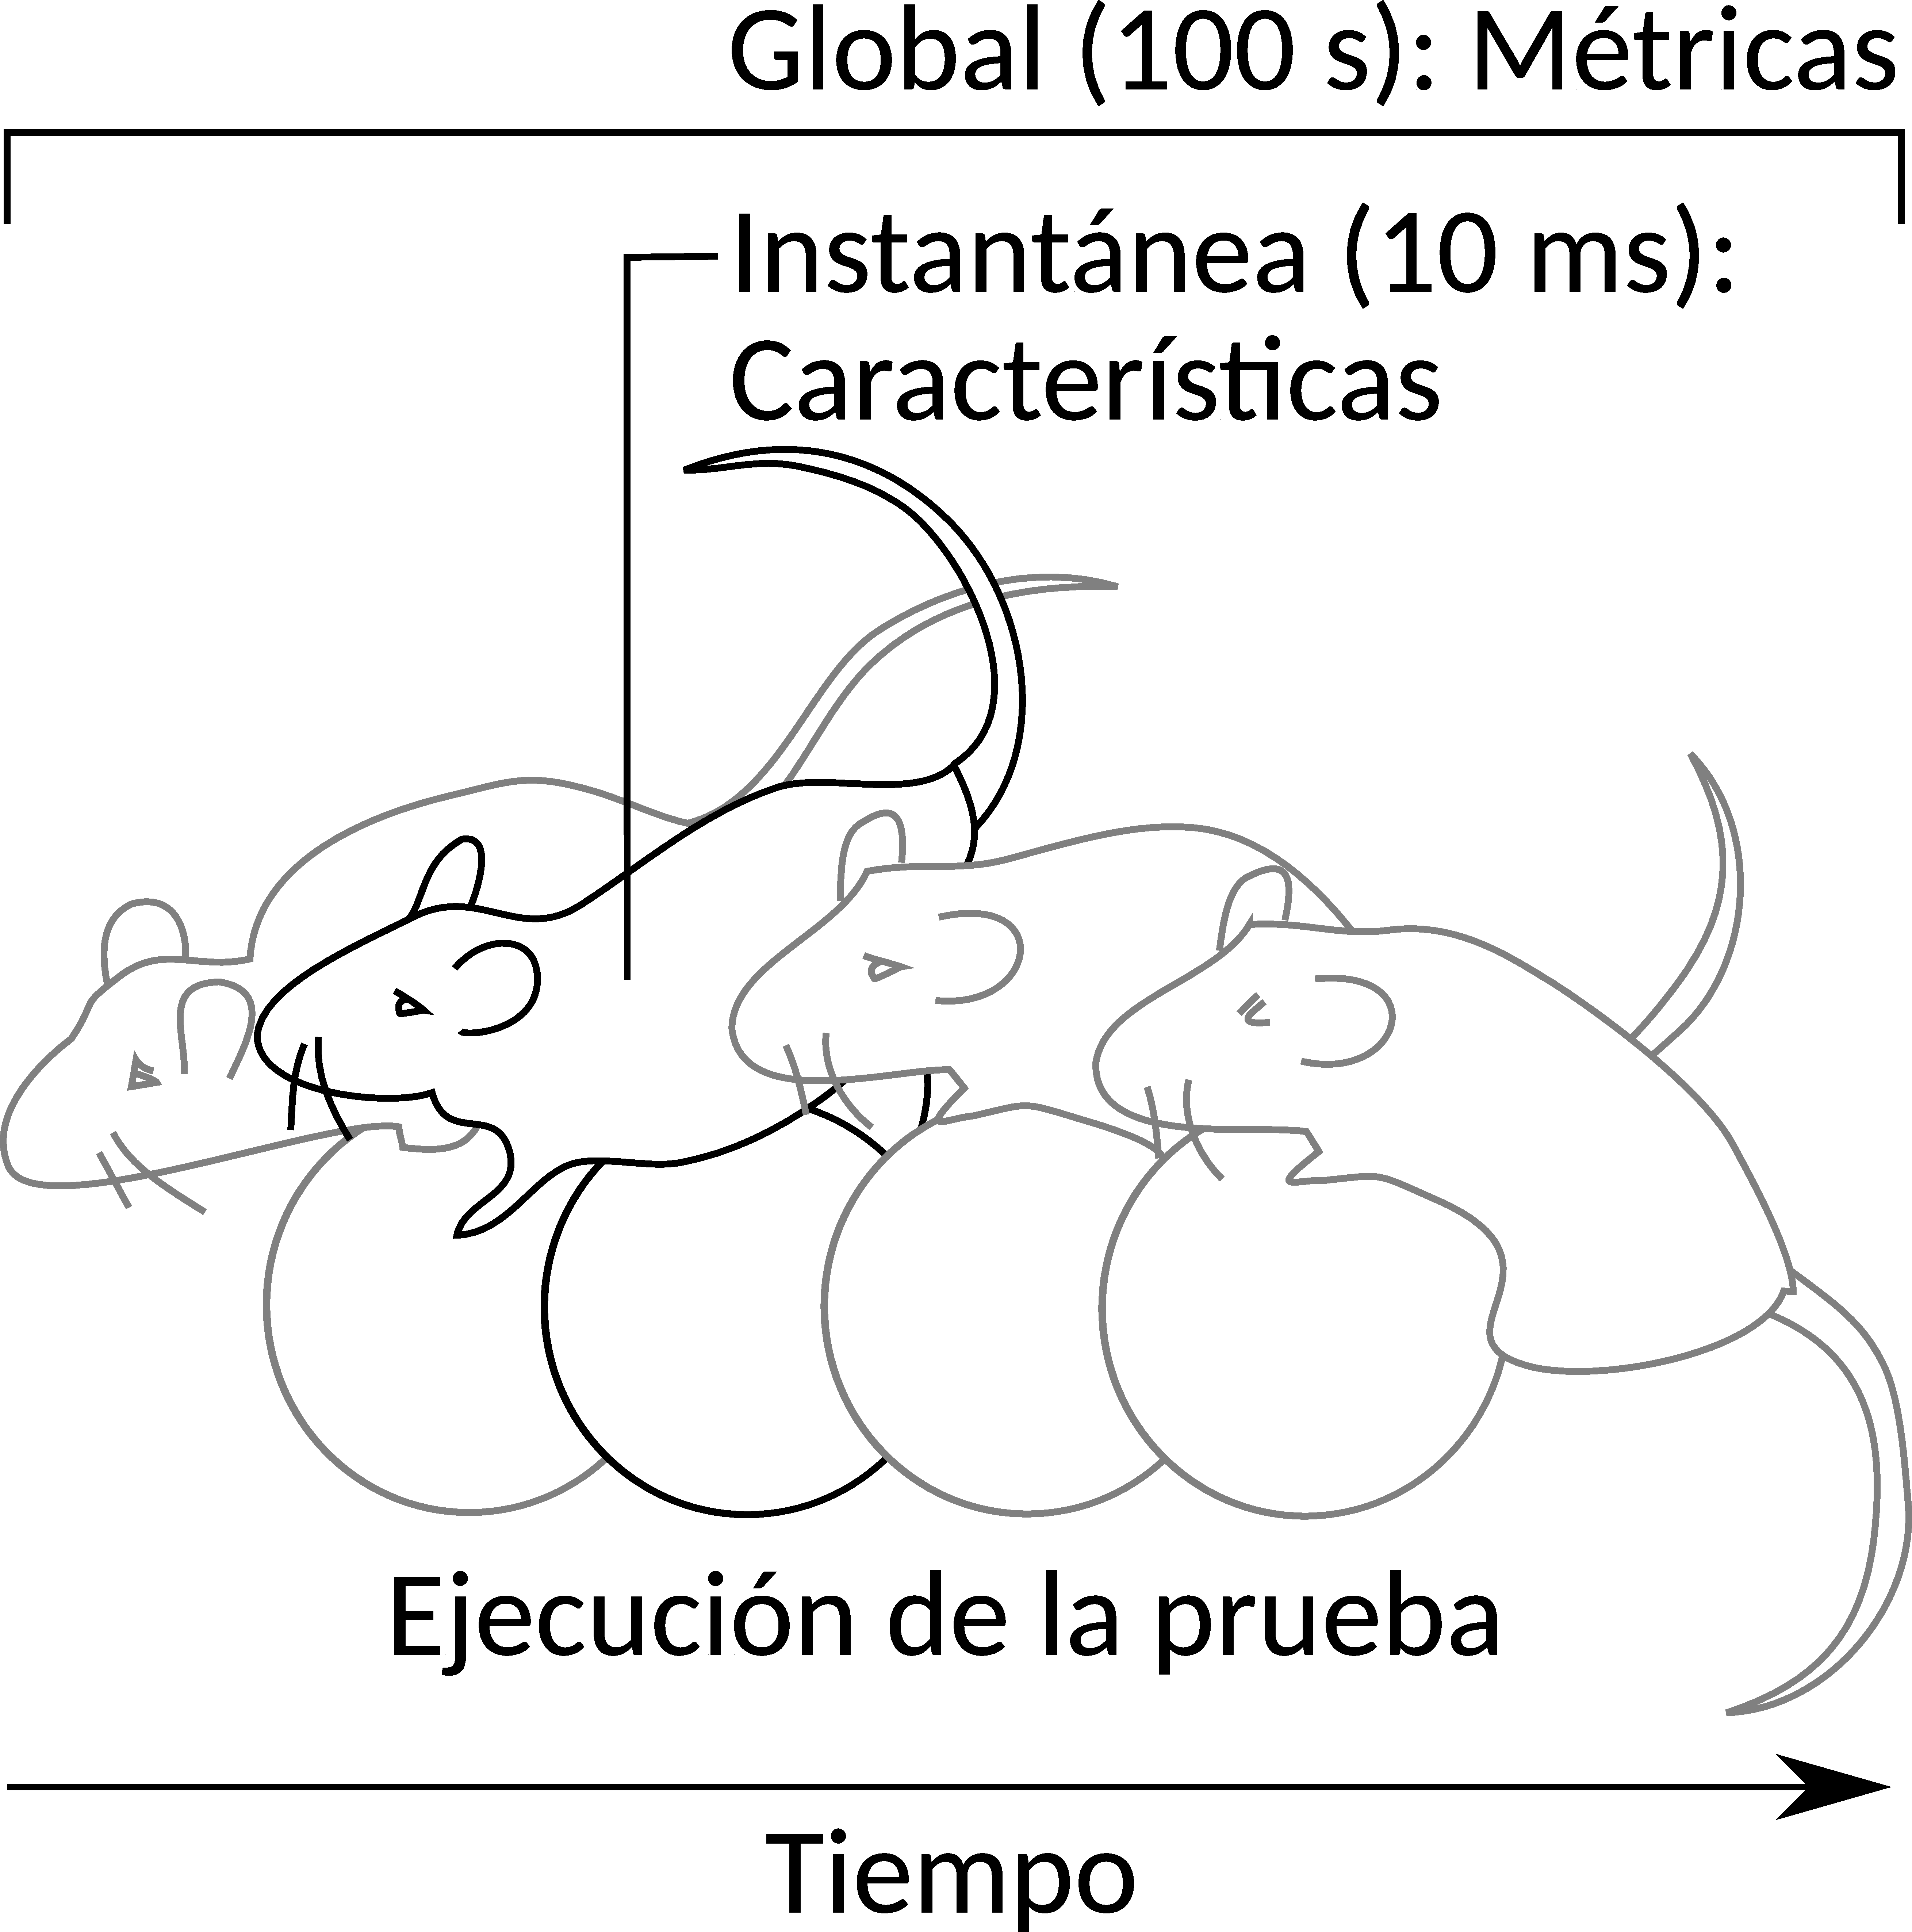
\includegraphics[width=0.45\linewidth]{figuras/capitulo3/representacion_comportamiento.pdf}
    \caption{\textbf{Escalas temporales en la descripción del comportamiento.} Ilustración de diferentes niveles de descripción del comportamiento animal, según la escala temporal de observación.}
    \label{fig:capitulo3_representacion_comportamiento}
\end{figure}

Formalmente, una métrica es una función que toma una realización de una prueba y devuelve un valor numérico
\begin{equation*}
    \text{Métrica comportamental}: \text{Prueba realizada} \mapsto \text{Valor} \in \mathbb{R}.
\end{equation*}

Por ejemplo, la latencia a caer es una de las métricas clásicas utilizadas para cuantificar el rendimiento en la tarea rotarod con aceleración. Para calcularla simplemente se determina el tiempo en que tarda un ratón en caerse del cilindro rotarod en una prueba. En la práctica, restringimos además la duración de cada prueba a un máximo de $300$ s, por lo que la latencia a caer es menor o igual a ese valor.

\clearpage

De acuerdo a los valores observados de latencia a caer, separamos a los individuos en dos grupos de rendimiento: 7 ratones de rendimiento bajo y 3 ratones de rendimiento alto (\autoref{fig:capitulo3_probabilidad_caer_por_rendimiento}). Los promedios de la latencia a caer de cada grupo se mantuvieron separados por una brecha de alrededor de 100 s (equivalente a entre 2 y 3 desviaciones estándar) durante todo el entrenamiento. Esta separación en grupos de rendimiento según la latencia a caer no se explica por el peso, sexo ni edad de los ratones, ya que estas condiciones eran homogéneas entre individuos. Sin embargo, podría depender del ritmo circadiano de los individuos, entre otros factores, si es que son más activos en diferentes momentos del día, ya que las pruebas rotarod se realizaron por la mañana de forma regular.

\begin{figure}[htbp]
    \centering
    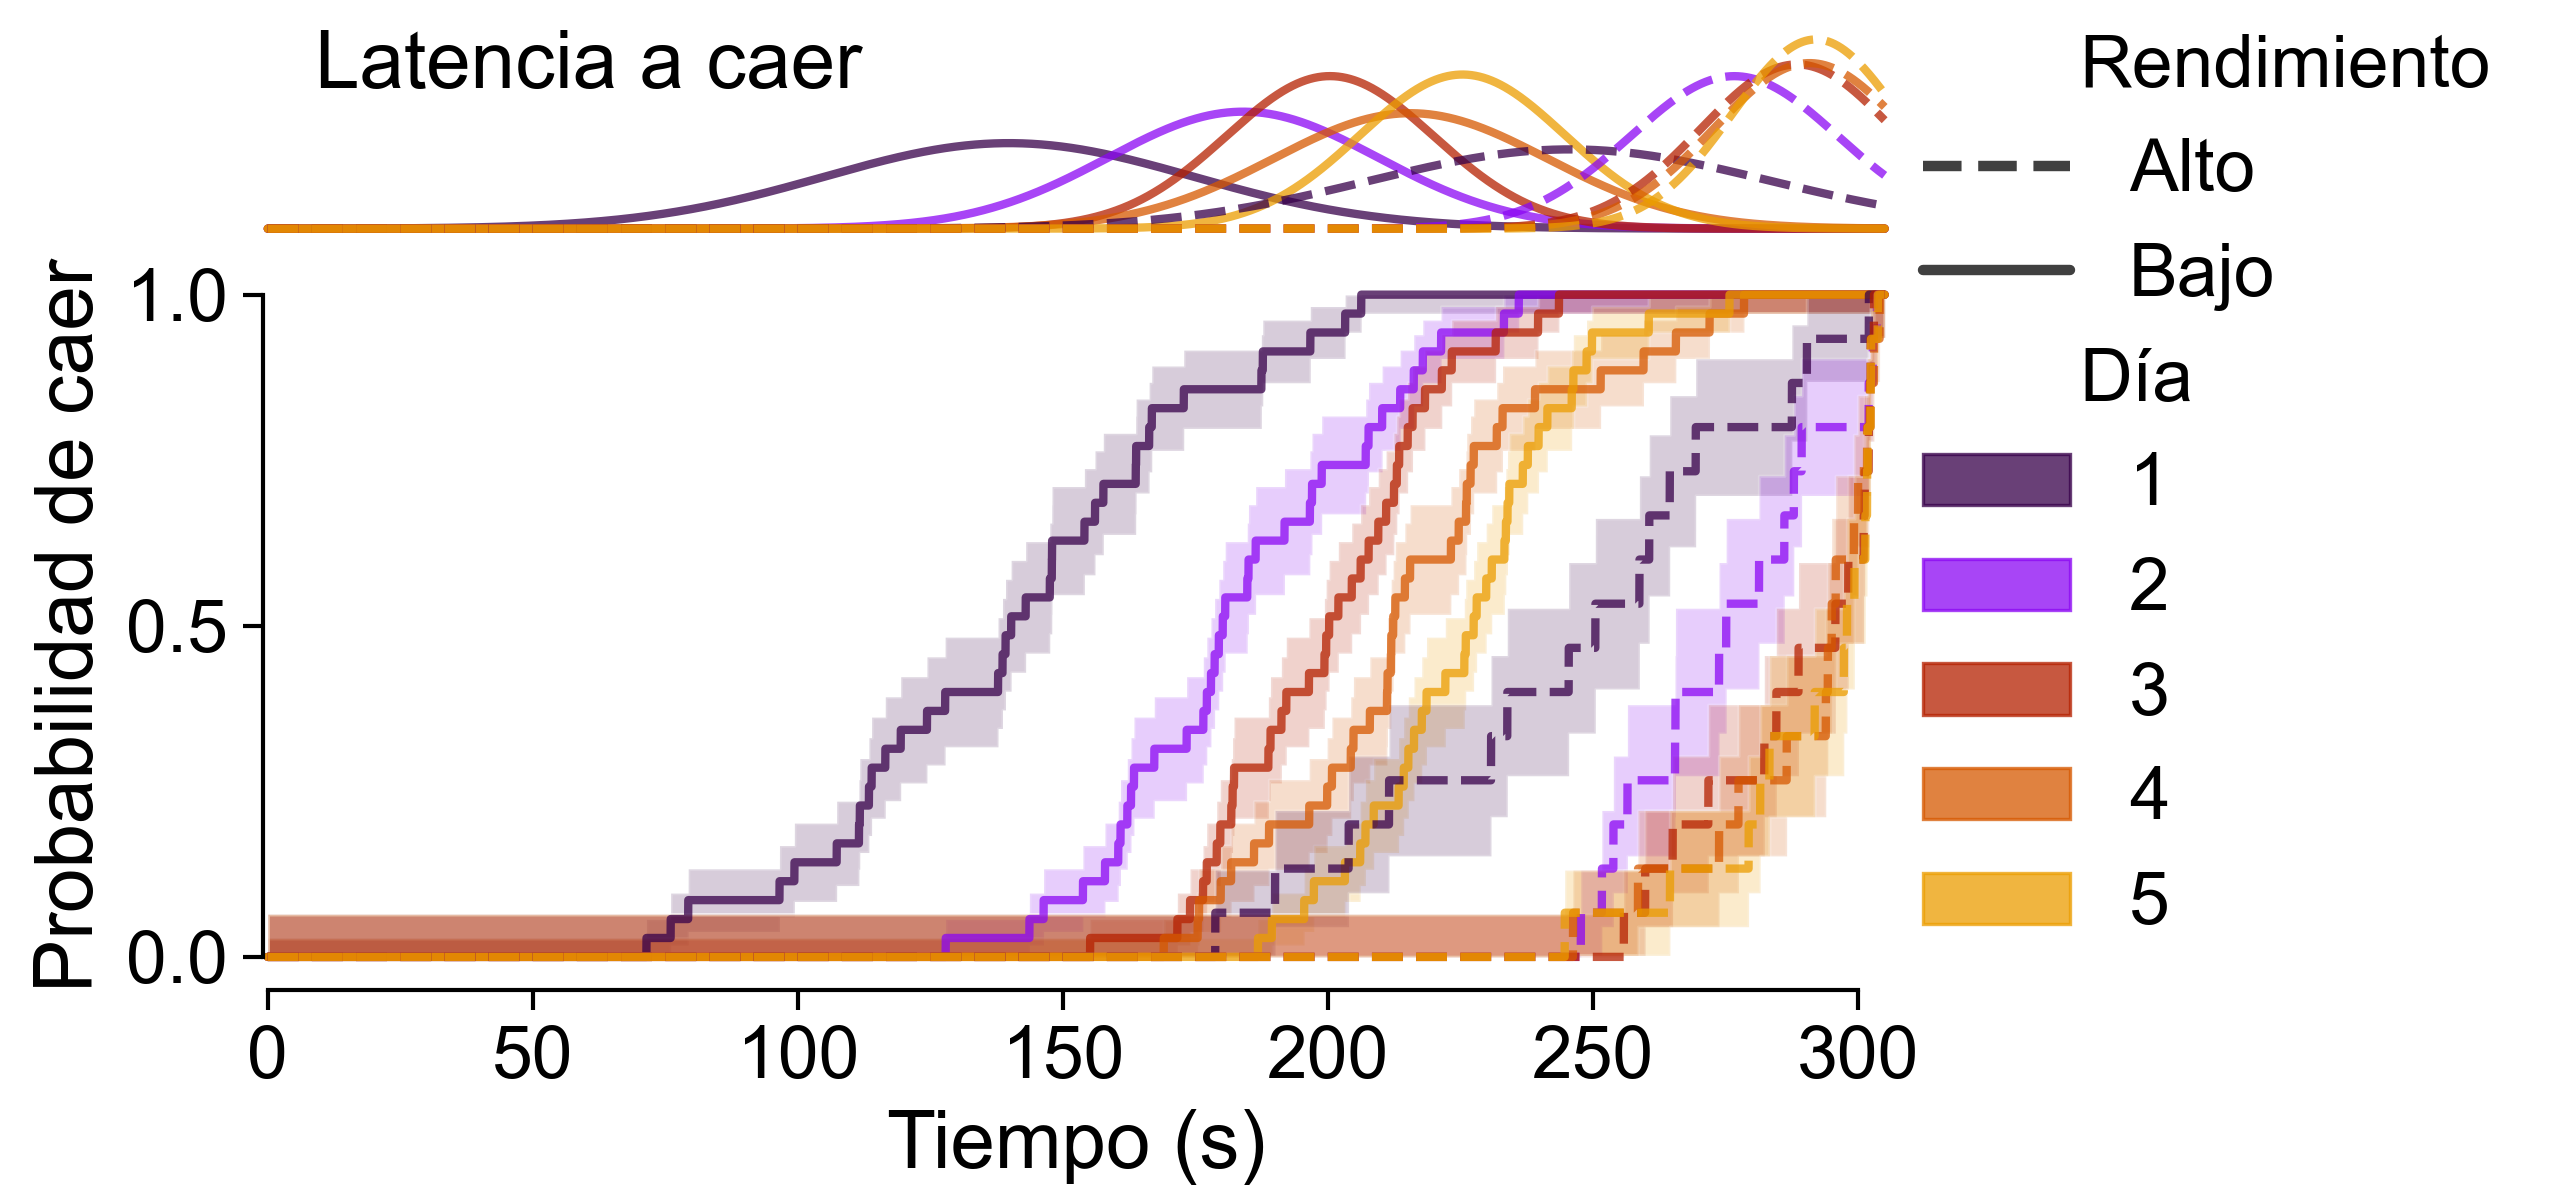
\includegraphics[width=0.8\linewidth]{figuras/capitulo3/probabilidad_caer_por_rendimiento.png}
    \caption{\textbf{Distribución de la latencia a caer.} (Abajo) Probabilidad de caer en un determinado tiempo de una prueba. (Arriba) Distribuciones de la latencia a caer.
        La latencia a caer aumenta con el día de entrenamiento y se observan dos grupos de ratones de diferente rendimiento.}
    \label{fig:capitulo3_probabilidad_caer_por_rendimiento}
\end{figure}

Otra métrica que se puede calcular es el valor promedio que adopta una característica comportamental durante una prueba. Sin embargo, la latencia a caer varía mucho (diferencias de 100 s) entre individuos, ya sea por su nivel de rendimiento o por su estadío de entrenamiento, por lo que tenemos registros bajo diferentes condiciones experimentales (la velocidad del cilindro rotarod aumenta con el tiempo). Por lo tanto, el promedio de la característica comportamental debe calcularse sobre tiempos donde se tengan registros de los individuos, bajo condiciones experimentales similares. Solamente 3 de las 250 pruebas realizadas tienen latencias a caer menores a 100 s, con una latencia a caer mínima observada de 70 s. Por estos motivos, calculamos los promedios dentro de los primeros 100 s de la tarea. También calculamos la pendiente con la que cambian las características de los pasos en estos primeros 100 s y el error en su ejecución.

Las características (conocidas también como \textit{features}) describen el comportamiento de manera más detallada. Las características comportamentales proporcionan información a escalas de tiempo sub-segundo, dependiendo de la resolución temporal experimental. Estas brindan una explicación detallada de la ejecución de una prueba, instante a instante, de manera aproximadamente continua. A su vez, estas descripciones a escalas de tiempo cortas pueden integrarse de diferentes maneras para dar origen a múlitples métricas comportamentales, que describen el comportamiento de manera global.

Un ejemplo de características comportamentales son las posiciones de las partes del cuerpo de los ratones, en nuestro caso medidas con una resolución temporal de $10$ ms. Otras características pueden ser los espectros de frecuencia \textit{wavelet} obtenidos de las partes del cuerpo de los ratones, u otras señales biofísicas. En particular, nosotros utilizaremos además de las posiciones de los marcadores, características que describen los pasos realizados por los ratones sobre el cilindro rotarod. Específicamente, las alturas mínima y máxima comprendidas en los pasos, su amplitud, velocidad instantánea, desfasaje entre las patas traseras y frecuencia entre pasos consecutivos de una misma pata.

Formalmente, una característica es una función que toma un tiempo determinado en una prueba y devuelve un valor numérico
\begin{equation*}
    \text{Característica comportamental}: \text{Tiempo} \mapsto \text{Valor} \in \mathbb{R}.
\end{equation*}

Por último, un conjunto de características comportamentales constituye una representación comportamental. El proceso de selección de características para representar el comportamiento depende de restricciones físicas, computacionales, experimentales o presupuestarias de cada laboratorio. En general, es conveniente utilizar una representación que sea sencilla y fácil de interpretar. Y que además incluya una cantidad características lo suficientemente grande para explicar detalladamente el comportamiento animal, pero lo suficientemente pequeña como para que el análisis sea computacionalmente eficiente
\begin{equation*}
    \text{Representación comportamental} = \{\text{Características comportamentales}\}.
\end{equation*}

A su vez, la representación comportamental elegida condiciona el tipo de información que se puede extraer en el análisis de la tarea. También podríamos representar el comportamiento usando un conjunto de métricas, como la latencia a caer, para describir el comportamiento en la escala temporal de la duración de las pruebas rotarod. Sin embargo, en este trabajo estudiaremos más adelante representaciones del comportamiento a escala temporal sub-segundo, para describir el comportamiento de los ratones durante cada instante de la tarea rotarod y construir mapas de comportamiento de dimensión reducida.

Finalmente, la ejecución de una prueba rotarod, vista a través de una característica en particular, son los valores de esa característica observados experimentalmente durante la tarea
\begin{align*}
    \text{Ejecución de una Prueba según una Característica} = & \ \{ \text{Característica(Tiempo)}         \\
                                                              & \ \text{para cada Tiempo de la Prueba} \}.
\end{align*}

A su vez, podemos juntar todas las características observadas durante una prueba, dentro de una representación comportamental dada, y llamar ejecución a este conjunto de observaciones
\begin{align*}
    \text{Ejecución de una Prueba} = & \ \{ \text{Característica(Tiempo)}               \\
                                     & \ \text{para cada Tiempo de la Prueba}           \\
                                     & \ \text{y para cada Característica}              \\
                                     & \ \text{de la Representacióń comportamental} \}.
\end{align*}

\clearpage

\section{Variación en las métricas por rendimiento y entrenamiento}\label{sec:variacion_metricas_grupo_rendimiento_dia_entrenamiento}

\begin{figure}[htbp]
    \centering
    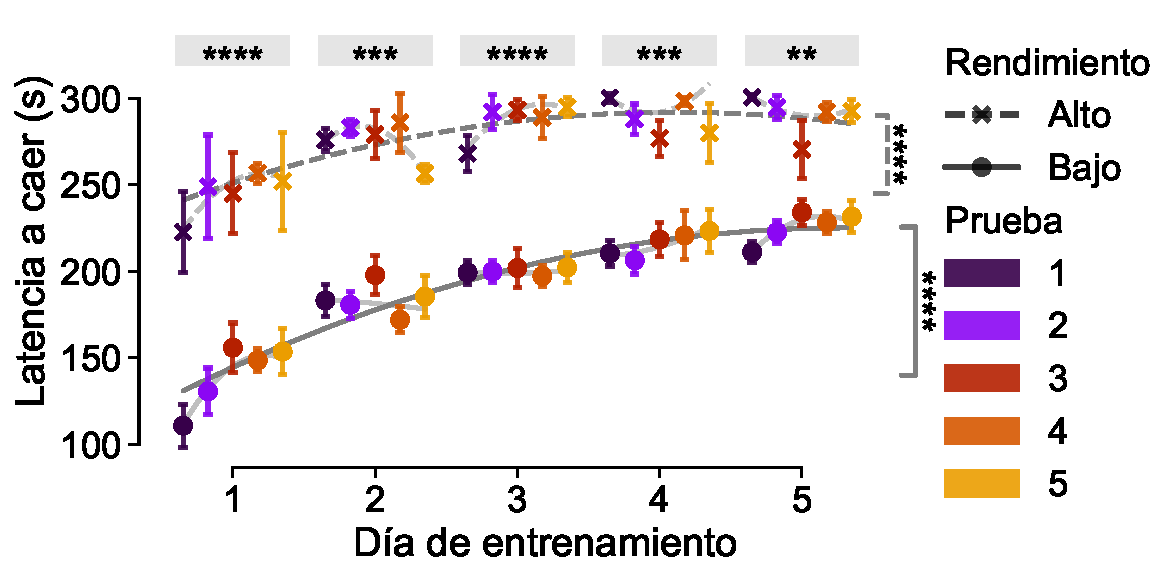
\includegraphics[width=0.8\linewidth]{figuras/capitulo3/latencia_por_prueba_por_rendimiento.pdf}
    \caption{\textbf{Latencia a caer por día y grupo de rendimiento.} La latencia a caer aumenta con el día de entrenamiento y se conserva una brecha entre los grupos de rendimiento.
        Los puntos muestran el promedio por grupo de rendimiento y las barras son el error estándar del promedio.
        Los rectángulos grises superiores indican los p-valores T-test entre grupos de rendimiento para cada día.
        Los corchetes en el margen derecho indican, para cada grupo de rendimiento, los p-valores \textit{one-way} ANOVA agrupando por día de entrenamiento.}
    \label{fig:capitulo3_latencia_por_prueba_por_rendimiento}
\end{figure}

Clásicamente, la latencia a caer es la métrica utilizada para evaluar el rendimiento y el aprendizaje motor en la tarea rotarod (\autoref{fig:capitulo3_latencia_por_prueba_por_rendimiento}). Nos interesa estudiar también cómo evolucionan otras métricas en función del día de entrenamiento y el grupo de rendimiento. Para ello, utilizaremos el Promedio$\{\xi\}$ (\autoref{fig:capitulo3_metricas_promedio}) y la Pendiente$\{\xi\}$ (\autoref{fig:capitulo3_metricas_pendiente}) de diferentes características de pasos $\xi$ durante los primeros 100 s de la tarea. Además, utilizaremos la raíz del error cuadrático medio RMSE$\{\xi\}$ (\autoref{fig:capitulo3_metricas_rmse}), para evaluar efectos del aprendizaje en la ejecución de la tarea. Calculamos este error como
\begin{equation*}
    \mathrm{RMSE}\{\xi\} = \sqrtexplained{%
    \langle \ \ \; \underbrace{[\hat{\mu}_{\xi}(t) - \mu^{\mathrm{fit}}_{\xi}(t)]^2}
    _{\substack{
            \text{Desviaciones}\\
            \text{respecto de una}\\
            \text{ejecución suave}
        }} + \underbrace{\hat{\sigma}_{\xi}^2(t)}
    _{\substack{
        \text{Varianza de}\\
        \text{la ejecución}\\
        \text{observada}
    }} \rangle
    } \, .
\end{equation*}

Identificamos dos términos que contribuyen al error de ejecución RMSE. Por un lado, un término de desviaciones respecto de la tendencia ajustada ($[\hat{\mu}_{\xi}(t) - \mu^{\mathrm{fit}}_{\xi}(t)]^2$), que representa la ``exactitud'' de la estrategia de locomoción. Y, por otro lado, un término de varianza ($\hat{\sigma}_{\xi}^2(t)$), que se interpreta como la ``precisión'' de la estrategia motora.

De esta manera, el error RMSE captura eventos en los que el ratón cambia súbitamente de estrategia de locomoción (por ejemplo, si tropieza o resbala), pues estos eventos producen desvíos grandes en $\hat{\mu}_x$ respecto de la tendencia ajustada $\mu^{\mathrm{fit}}_x$. Esto se debe a que la tendencia ajustada $\mu^{\mathrm{fit}}_{\xi}$ (polinomio de grado 3) es mucho más suave que $\hat{\mu}_{\xi}$, como función del tiempo $t$, por lo que no varía bruscamente frente a estos eventos de cambio de estrategia. Además, el error RMSE toma en cuenta la variablidad intrínseca de la característica $\xi$, a través de su varianza $\hat{\sigma}_{\xi}^2(t)$. Intuitivamente, el error RMSE cuantifica qué tanto se desvía la estrategia de locomoción del ratón, respecto de una estrategia que varía de manera suave y que se ejecuta de manera precisa.

Para el cálculo de las métricas Promedio, Pendiente y RMSE, promediamos las características $\xi$ las patas izquierda y derecha. De esta manera eliminamos las variaciones por lateralidad que puedan tener los ratones, por ejemplo por tener una pata dominante. Al promediar las características entre las patas ignoramos también estrategias de comportamiento asimétricas, por ejemplo si el ratón se mueve inclinado respecto de la horizontal del cilindro. Esto lo hacemos para simplificar esta parte del análisis, a pesar de la pérdida de información detallada de la estrategia de locomoción.

Respecto a los resultados obtenidos (Figuras \ref{fig:capitulo3_metricas_promedio}, \ref{fig:capitulo3_metricas_pendiente} y \ref{fig:capitulo3_metricas_rmse} suplementarias), en general el grupo de 7 ratones de bajo rendimiento muestra cambios estadísticamente más significativos durante el entrenamiento, comparado con el grupo de 3 ratones de alto rendimiento (\autoref{tab:pvalores-anova}). Esta mayor significancia estadística se explica tanto por el mayor número de ratones en el grupo de bajo rendimiento, como también por la mayor magnitud de los cambios en los valores de las métricas a lo largo de los días de entrenamiento, frente a las fluctuaciones intra-día. En particular, en las métricas Promedio, Pendiente y RMSE calculadas a partir de la Altura mínima, Altura máxima y Frecuencia muestran los cambios más significativos con el aprendizaje, para el grupo de bajo rendimiento. Mientras que para el grupo de alto rendimiento, las métricas Promedio y RMSE (no así la Pendiente) presentan los cambios más significativos cuando son calculadas a partir de la Altura máxima y la Frecuencia de los pasos.

En general, las mayores variaciones interprueba en las métricas ocurren más frecuentemente en la prueba D1T2, respecto de la prueba inmediatamente anterior D1T1 (\autoref{tab:variacion-interpureba}). Más detalladamente, en la prueba D1T2 se observaron las mayores variaciones en 5 de las 6 métricas RMSE, en 2 de las 6 métricas Promedio y en ninguna de las métricas Pendiente. Finalmente, las métricas Latencia a caer y Promedio\{Amplitud\} sufren su mayor cambio en la prueba D2T1, respecto de la prueba inmediatamente anterior D1T5 (\autoref{tab:variacion-interpureba}).

De esta manera, la mayoría de las métricas RMSE, la mitad de las Promedio y la Latencia a caer sufren cambios significativos de manera relativamente temprana, durante el comienzo del primer y segundo día del proceso de entrenamiento. Por su parte, la mayoría de las métricas Pendiente sufren cambios significativos más tardíos, ocurriendo las mayores variaciones en la prueba D3T1 (3 de las 6 métricas) y en la prueba D5T1 (2 de las 6 métricas). Además, la otra mitad de las métricas Promedio y una de las RMSE sufren cambios tardíos.

En cuanto a las diferencias entre los grupos de rendimiento, estas son más significativas al comienzo (D1 y D2) y al final (D5) del entrenamiento, según la mayoría de las métricas (\autoref{tab:pvalores-t-test}). Todas las métricas Promedio y 4 de las 6 métricas RMSE muestran diferencias significativas entre los grupos de rendimiento en todos los días. En cuanto a las métricas Pendiente, se observan diferencias significativas entre los grupos de rendimiento en 5 de estas 6 métricas en el día D1, en 3 de 6 en el día D2 y en 4 de 6 en el día D5. En particular, las métricas Pendiente\{Altura máxima\} y Pendiente\{Desfasaje\} comienzan con diferencias significativas entre los grupos de rendimiento en el día D1, y estas diferencias se hacen menos significativas con el entrenamiento. En general, la característica Frecuencia muestra diferencias menos significativas que el resto de las características, para todas las métricas.

En resumen, el método más tradicional de representación del comportamiento, la métrica de latencia a caer, captura el progreso de los animales durante el entrenamiento y también las diferencias entre animales según su aptitud física previa. Adicionalmente, conseguimos definir otras métricas que describir de manera global cómo se desempeñan los ratones en la tarea. De esta manera aportamos más información sobre el comportamiento de los ratones. Vimos que no solo aumenta la latencia a caer con el entrenamiento, sino que también aumentan la altura a la que los ratones dan pasos sobre el cilindro rotarod, mientras que la amplitud y la velocidad de los pasos se reduce (\autoref{fig:capitulo3_metricas_promedio}). Además, los ratones de bajo rendimiento aprenden a mantenerse más arriba del cilindro, reduciendo la tendencia a que la rotación del cilindro los arrastre hacia abajo (\autoref{fig:capitulo3_metricas_pendiente} Pendiente de la Altura mínima y de la Altura máxima). Registramos que los errores en las ejecuciones comportamentales de los ratones se reduce con el entrenamiento (\autoref{fig:capitulo3_metricas_rmse}). Observamos que la mayoría de los cambios más significativos en estas métricas se dan en la segunda prueba del primer día de entrenamiento, mostrando la rapidez con la que los ratones se adaptan a nuevos entornos. El desfasaje entre los pasos de las patas traseras no cambia significativamente durante el entrenamiento.

A su vez, la mayoría de las métricas alternativas estudiadas separan a los ratones en 2 grupos de rendimiento: 7 ratones de bajo rendimiento y 3 ratones de alto rendimiento. Estos grupos de rendimiento se definieron con base a la latencia a caer exhibida por los ratones, habiendo una maracada brecha desde el primer día de entrenamiento que se mantuvo hasta el día cinco, el último día de entrenamiento registrado.

Las variaciones de las métricas alternativas a la latencia a caer son más visibles en el grupo de ratones de bajo rendimiento. Sin embargo, debido a la alta variabilidad intra-día de las métricas, al realizar un ANOVA de las métricas a lo largo del entrenamiento, solamente la Altura mínima, la Altura máxima y la Frecuencia de los pasos cambia de manera estadísticamente significativa, de manera más consistente al calcular su Promedio, Pendiente y error de ejecución RMSE durante los primeros 100 s de las pruebas rotarod. Esto no quita que la existencia de cambios, aunque sea sutiles, en el resto de las métricas, aunque quedan enmascarados por la alta variabilidad entre pruebas en un mismo día (Figuras \ref{fig:capitulo3_metricas_promedio}, \ref{fig:capitulo3_metricas_pendiente} y \ref{fig:capitulo3_metricas_rmse} suplementarias). Respecto a la variabilidad intra-día, esta podría deberse a un proceso de fatiga o a un aprendizaje a corta escala temporal, pero para determinar su origen hacen falta más estudios teniendo en cuenta esos factores.

En el capítulo siguiente introducimos mapas de comportamiento usando el algoritmo UMAP de reducción de la dimensión. Esta es una manera de visualizar, de manera resumida, la información de un conjunto de múltiples características comportamentales. Decimos que los conjuntos de características de los que partimos son de dimensión alta (en nuestro caso, entre 30 y 50 dimensiones), en contraste con el mapa UMAP obtenido, que es una representación resumida del sistema, en una proyección de 2 dimensiones.

\begin{table}[htbp]
    \centering
    \begin{tabular}{clcc}
                                                                      &                   & \multicolumn{2}{c}{\textbf{Rendimiento}}                               \\ \cline{3-4}
                                                                      & \textbf{Métricas} & \textbf{Bajo}                            & \textbf{Alto}               \\ \cline{2-4}
                                                                      & Latencia a caer   & $\mathbf{1\times 10^{-30}}$              & $\mathbf{1\times 10^{-6}}$  \\ \cline{2-4}
        \multirow{6}{*}{\rotatebox[origin=c]{90}{\textbf{Promedio}}}  & Altura mínima     & $\mathbf{5\times 10^{-3}}$               & 0.12                        \\
                                                                      & Altura máxima     & $\mathbf{1\times 10^{-7}}$               & $\mathbf{9\times 10^{-3}}$  \\
                                                                      & Amplitud          & 0.34                                     & 0.42                        \\
                                                                      & Velocidad         & 0.49                                     & 0.49                        \\
                                                                      & Desfasaje         & 0.25                                     & \textbf{0.034}              \\
                                                                      & Frecuencia        & $\mathbf{6\times 10^{-4}}$               & $\mathbf{10\times 10^{-4}}$ \\ \cline{2-4}
        \multirow{6}{*}{\rotatebox[origin=c]{90}{\textbf{Pendiente}}} & Altura mínima     & $\mathbf{2\times 10^{-5}}$               & 0.44                        \\
                                                                      & Altura máxima     & $\mathbf{4\times 10^{-11}}$              & 0.53                        \\
                                                                      & Amplitud          & \textbf{0.035}                           & 0.51                        \\
                                                                      & Velocidad         & 0.068                                    & 0.69                        \\
                                                                      & Desfasaje         & 0.61                                     & \textbf{0.011}              \\
                                                                      & Frecuencia        & \textbf{0.011}                           & 0.99                        \\ \cline{2-4}
        \multirow{6}{*}{\rotatebox[origin=c]{90}{\textbf{RMSE}}}      & Altura mínima     & 0.072                                    & 0.065                       \\
                                                                      & Altura máxima     & $\mathbf{5\times 10^{-6}}$               & $\mathbf{5\times 10^{-4}}$  \\
                                                                      & Amplitud          & 0.072                                    & 0.081                       \\
                                                                      & Velocidad         & 0.46                                     & 0.19                        \\
                                                                      & Desfasaje         & 0.055                                    & 0.21                        \\
                                                                      & Frecuencia        & $\mathbf{4\times 10^{-4}}$               & \textbf{0.032}
    \end{tabular}
    \caption{\textbf{Cambios más significativos en el grupo de bajo rendimiento.} p-valores \textit{one-way} ANOVA para medir cambios a lo largo de los días de entrenamiento, para cada grupo de rendimiento. Los p-valores estadísticamente significativos se indican en negrita.}
    \label{tab:pvalores-anova}
\end{table}

\begin{table}[htbp]
    \centering
    \begin{tabular}{clcccc}
                                                                      &                                   & \multicolumn{4}{c}{\textbf{Mayor variación interprueba}}                                                                  \\ \cline{3-6}
                                                                      & \textbf{Métricas}                 & \textbf{Pruebas}                                         & \textbf{Nominal} & \textbf{Porcentual (\%)} & \textbf{Z-score} \\ \cline{2-6}
                                                                      & Latencia a caer (s)               & \bf D2T1                                                 & 30(16)           & 24(13)                   & 1.8              \\ \cline{2-6}
        \multirow{6}{*}{\rotatebox[origin=c]{90}{\textbf{Promedio}}}  & Altura mínima (mm)                & \bf D1T2                                                 & 3.2(2.3)         & 47(33)                   & 1.4              \\
                                                                      & Altura máxima (mm)                & \bf D1T2                                                 & 2.6(0.9)         & 60(20)                   & 3.0              \\
                                                                      & Amplitud (mm)                     & D2T1                                                     & -2.0(2.2)        & -60(67)                  & 0.9              \\
                                                                      & Velocidad (mm s$^{-1}$)           & D4T1                                                     & -28(28)          & -66(66)                  & 1.0              \\
                                                                      & Desfasaje (vueltas)               & D3T5                                                     & 0.012(0.015)     & 29(36)                   & 0.8              \\
                                                                      & Frecuencia (Hz)                   & \bf D4T5                                                 & -0.14(0.06)      & -30(13)                  & 2.3              \\ \cline{2-6}
        \multirow{6}{*}{\rotatebox[origin=c]{90}{\textbf{Pendiente}}} & Altura mínima (mm hs$^{-1}$)      & \bf D3T1                                                 & 5.1(2.1)         & 58(24)                   & 2.4              \\
                                                                      & Altura máxima (mm hs$^{-1}$)      & \bf D2T4                                                 & 1.2(0.6)         & 34(16)                   & 2.1              \\
                                                                      & Amplitud (mm hs$^{-1}$)           & \bf D3T1                                                 & -4.8(1.7)        & -77(27)                  & 2.9              \\
                                                                      & Velocidad (mm s$^{-1}$ hs$^{-1}$) & \bf D3T1                                                 & -81(25)          & -93(29)                  & 3.2              \\
                                                                      & Desfasaje (vueltas hs$^{-1}$)     & \bf D5T1                                                 & -0.085(0.051)    & -73(43)                  & 1.7              \\
                                                                      & Frecuencia (Hz hs$^{-1}$)         & \bf D5T1                                                 & -0.29(0.08)      & -80(22)                  & 3.6              \\ \cline{2-6}
        \multirow{6}{*}{\rotatebox[origin=c]{90}{\textbf{RMSE}}}      & Altura mínima (mm)                & \bf D1T2                                                 & -1.4(0.3)        & -75(17)                  & 4.3              \\
                                                                      & Altura máxima (mm)                & \bf D1T2                                                 & -1.1(0.5)        & -47(22)                  & 2.1              \\
                                                                      & Amplitud (mm)                     & \bf D1T2                                                 & -1.0(0.4)        & -60(22)                  & 2.7              \\
                                                                      & Velocidad (mm s$^{-1}$)           & \bf D1T2                                                 & -12(5)           & -68(29)                  & 2.3              \\
                                                                      & Desfasaje (vueltas)               & \bf D3T4                                                 & -0.010(0.005)    & -44(21)                  & 2.0              \\
                                                                      & Frecuencia (Hz)                   & \bf D1T2                                                 & -0.20(0.07)      & -58(20)                  & 2.9
    \end{tabular}
    \caption{\textbf{Mayoría de cambios ocurren en la prueba D1T2.} Pruebas en las que se observó la mayor variación en el Z-score de las métricas, respecto de la prueba inmediatamente anterior. Se muestran los resultados del grupo de ratones de bajo rendimiento. Las pruebas con Z-scores mayores a 1 se indican en negrita. El símbolo D$i$T$j$ denota la prueba $j$ del día $i$.}
    \label{tab:variacion-interpureba}
\end{table}

\begin{table}[htbp]
    \centering
    \begin{tabular}{clccccc}
                                                                      &                   & \multicolumn{5}{c}{\textbf{Día de entrenamiento}}                                                                                                                     \\ \cline{3-7}
                                                                      & \textbf{Métricas} & \textbf{D1}                                       & \textbf{D2}                & \textbf{D3}                & \textbf{D4}                & \textbf{D5}                \\ \cline{2-7}
                                                                      & Latencia a caer   & $\mathbf{3\times 10^{-5}}$                        & $\mathbf{3\times 10^{-4}}$ & $\mathbf{5\times 10^{-5}}$ & $\mathbf{4\times 10^{-4}}$ & $\mathbf{2\times 10^{-3}}$ \\ \cline{2-7}
        \multirow{6}{*}{\rotatebox[origin=c]{90}{\textbf{Promedio}}}  & Altura mínima     & $\mathbf{5\times 10^{-5}}$                        & $\mathbf{2\times 10^{-6}}$ & $\mathbf{9\times 10^{-6}}$ & $\mathbf{2\times 10^{-4}}$ & $\mathbf{1\times 10^{-4}}$ \\
                                                                      & Altura máxima     & $\mathbf{3\times 10^{-3}}$                        & $\mathbf{2\times 10^{-6}}$ & $\mathbf{2\times 10^{-4}}$ & $\mathbf{3\times 10^{-5}}$ & $\mathbf{1\times 10^{-5}}$ \\
                                                                      & Amplitud          & $\mathbf{2\times 10^{-3}}$                        & $\mathbf{1\times 10^{-5}}$ & $\mathbf{3\times 10^{-6}}$ & $\mathbf{4\times 10^{-4}}$ & $\mathbf{2\times 10^{-4}}$ \\
                                                                      & Velocidad         & $\mathbf{2\times 10^{-3}}$                        & $\mathbf{5\times 10^{-5}}$ & $\mathbf{2\times 10^{-5}}$ & $\mathbf{5\times 10^{-4}}$ & $\mathbf{2\times 10^{-4}}$ \\
                                                                      & Desfasaje         & $\mathbf{9\times 10^{-3}}$                        & $\mathbf{2\times 10^{-3}}$ & $\mathbf{2\times 10^{-3}}$ & $\mathbf{2\times 10^{-3}}$ & $\mathbf{2\times 10^{-4}}$ \\
                                                                      & Frecuencia        & \textbf{0.012}                                    & \textbf{0.022}             & \textbf{0.010}             & \textbf{0.012}             & \textbf{0.022}             \\ \cline{2-7}
        \multirow{6}{*}{\rotatebox[origin=c]{90}{\textbf{Pendiente}}} & Altura mínima     & $\mathbf{8\times 10^{-3}}$                        & \textbf{0.032}             & 0.65                       & 0.17                       & \textbf{0.017}             \\
                                                                      & Altura máxima     & \textbf{0.016}                                    & 0.25                       & 0.15                       & 0.37                       & 0.084                      \\
                                                                      & Amplitud          & $\mathbf{4\times 10^{-3}}$                        & \textbf{0.021}             & 0.31                       & 0.073                      & $\mathbf{3\times 10^{-3}}$ \\
                                                                      & Velocidad         & $\mathbf{3\times 10^{-3}}$                        & \textbf{0.015}             & 0.22                       & 0.052                      & $\mathbf{3\times 10^{-3}}$ \\
                                                                      & Desfasaje         & \textbf{0.028}                                    & 0.11                       & 0.39                       & 0.48                       & 0.49                       \\
                                                                      & Frecuencia        & 0.59                                              & 0.64                       & 0.65                       & 0.57                       & \textbf{0.021}             \\ \cline{2-7}
        \multirow{6}{*}{\rotatebox[origin=c]{90}{\textbf{RMSE}}}      & Altura mínima     & $\mathbf{2\times 10^{-3}}$                        & $\mathbf{1\times 10^{-5}}$ & $\mathbf{1\times 10^{-3}}$ & $\mathbf{6\times 10^{-4}}$ & $\mathbf{4\times 10^{-3}}$ \\
                                                                      & Altura máxima     & \textbf{0.013}                                    & $\mathbf{3\times 10^{-5}}$ & $\mathbf{5\times 10^{-3}}$ & $\mathbf{3\times 10^{-4}}$ & $\mathbf{2\times 10^{-3}}$ \\
                                                                      & Amplitud          & $\mathbf{2\times 10^{-3}}$                        & $\mathbf{3\times 10^{-5}}$ & $\mathbf{4\times 10^{-4}}$ & $\mathbf{1\times 10^{-3}}$ & $\mathbf{2\times 10^{-3}}$ \\
                                                                      & Velocidad         & $\mathbf{5\times 10^{-4}}$                        & $\mathbf{3\times 10^{-4}}$ & $\mathbf{2\times 10^{-4}}$ & $\mathbf{5\times 10^{-4}}$ & $\mathbf{2\times 10^{-3}}$ \\
                                                                      & Desfasaje         & 0.58                                              & 0.49                       & 0.67                       & 0.95                       & 0.70                       \\
                                                                      & Frecuencia        & 0.49                                              & 0.61                       & 0.26                       & 0.61                       & 0.90
    \end{tabular}
    \caption{\textbf{Mayoría de métricas separan los grupos de rendimiento.} p-valores T-test entre grupos de rendimiento. Los p-valores estadísticamente significativos se indican en negrita. El símbolo D$i$ denota el día $i$.}
    \label{tab:pvalores-t-test}
\end{table}
\chapter{Mapas de comportamiento}\label{cha:mapas_comportamiento}

\AddToShipoutPictureBG*{\put(0,0){%
        \parbox[b][\paperheight]{\paperwidth}{%
            \vfill
            \centering
            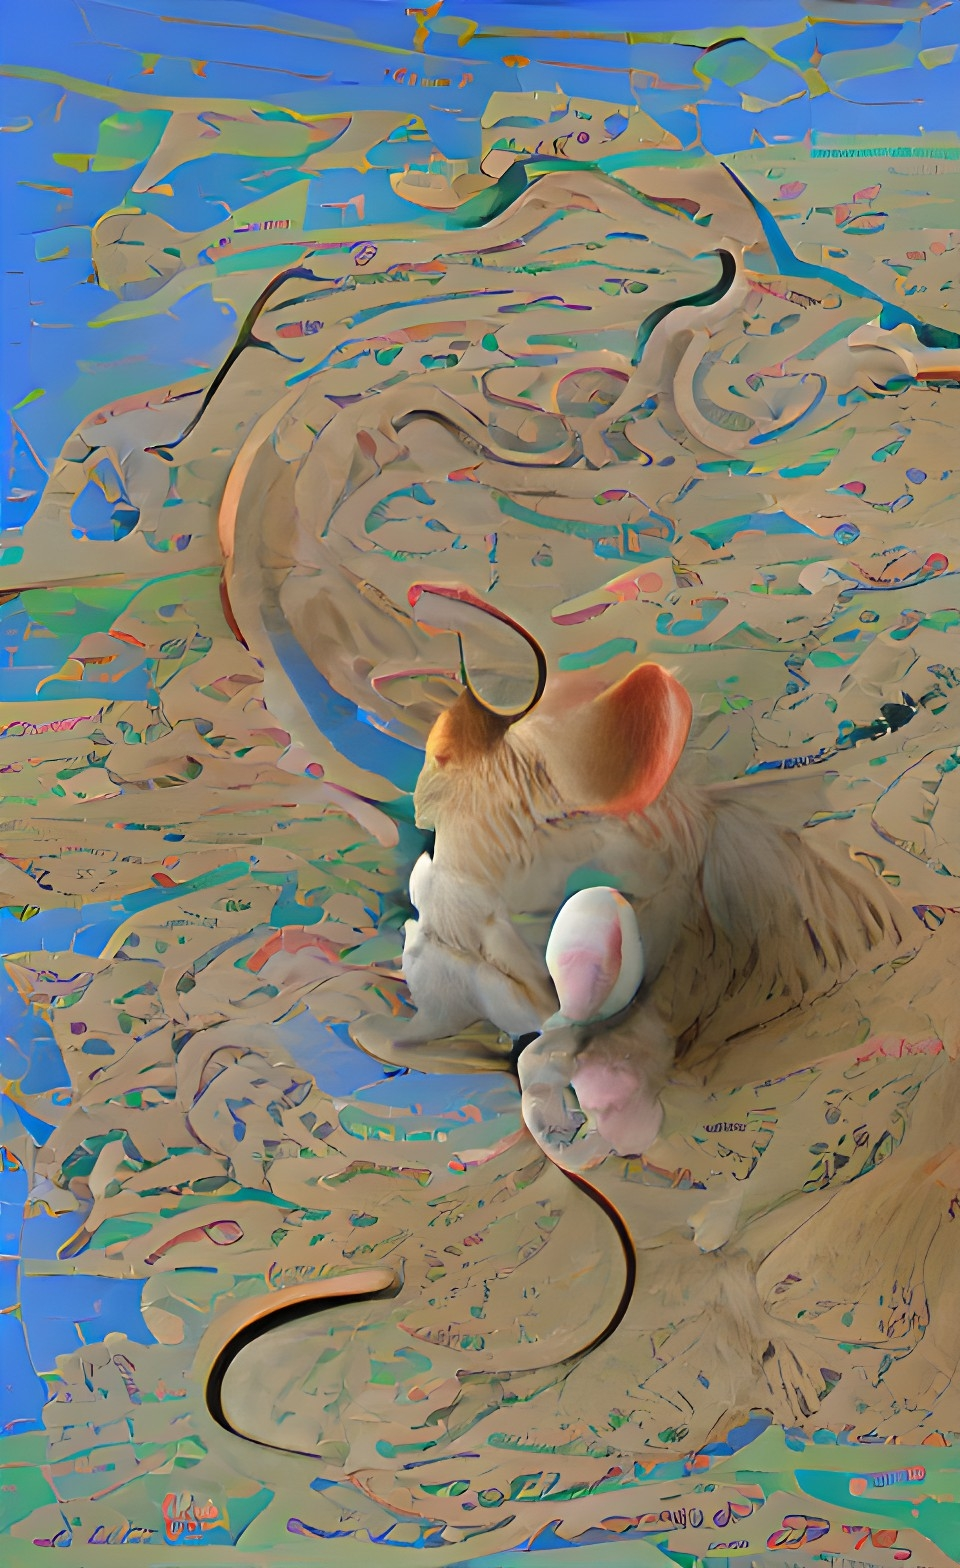
\includegraphics[width=\paperwidth,height=\paperheight,keepaspectratio]{%
                figuras/caratulas/mapa_de_comportamientos.jpg}\vfill
        }}}

\AddToShipoutPicture*{
    \begin{tikzpicture}[overlay, remember picture]
        \fill[white, opacity=0.75] (20, 24) rectangle (1, 21);
    \end{tikzpicture}}

\clearpage

Cuantificar el comportamiento animal es fundamental para el análisis de su correlación con la actividad neuronal con el fin de estudiar cómo el cerebro codifica diferentes comportamientos, cuáles son los circuitos neuronales subyacentes y cómo estos se modifican durante el aprendizaje de nuevas tareas motoras \cite{esposito_defensive, levy_representation}. En general, se necesita una amplia variedad de características para capturar detalladamente las sutilezas del comportamiento animal complejo en un experimento. Debido a que esta alta dimensionalidad en los datos puede resultar inconveniente para su análisis, frecuentemente se utilizan técnicas de reducción de la dimensión sobre los conjuntos de características comportamentales. Estas técnicas generan representaciones de menor dimensión que capturan la mayor parte de la varianza y/o la mayoría de las relaciones de similaridad locales de los datos, es decir, son una buena aproximación del conjunto de datos original. Además, muchas de estas técnicas, como el análisis de componentes principales (\textit{Principal Component Analysis}, PCA), son utilizadas comúnmente en el estudio de registros de actividad neuronal. El algoritmo de PCA identifica un conjunto ordenado de componentes principales (PCs), que constituyen diferentes ejes ortogonales sobre los que se puede descomponer al conjunto de datos. Cada PC captura progresivamente menos varianza en los datos y, por lo tanto, aporta progresivamente menos información, siendo la primera componente principal (PC1) la que captura la mayor proporción de la varianza en los datos. De esta manera, un subconjunto de PCs puede utilizarse para reconstruir de manera aproximada a las características comportamentales subyacentes y usando un menor número de variables en total \cite{datta_computational_neuroethology}.

Sin embargo, por ser una transformación lineal, PCA solo es capaz de capturar relaciones globales a grandes rasgos en la estructura interna de los datos comportamentales. Para respetar mejor la estructura latente del comportamiento a nivel local se pueden utilizar técnicas no lineales de reducción de la dimensión. Algunos de estos algoritmos se basan en construir representaciones que respeten la topología del conjunto de datos original, y luego proyectar esta representación topológica en un espacio de dimensión menor (por lo general en 2 dimensiones, para facilitar su visualización). Estos métodos basados en grafos suelen ser preferibles por encima de los métodos lineales porque capturan la estructura local de los datos, lo cual permite describir detalladamente comportamientos sutiles usando muy pocas dimensiones. Recientemente, la utilidad de estos métodos ha cobrado protagonismo en diversas áreas de investigación en biología y forman parte de las herramientas fundacionales de la neuroetología computacional \cite{sainburg_birdsong_umap}.

En este trabajo, utilizamos proyecciones UMAP (\textit{Uniform Manifold Approximation and Projection}) para describir la actividad de ratones durante la ejecución de la tarea rotarod e inferir categorías comportamentales subyacentes, de manera no supervisada \cite{mcinnes_umap}. El algoritmo UMAP se usó para encontrar proyecciones en 2 dimensiones de conjuntos de datos. La estructura de los datos en este espacio de dimensión baja respeta su estructura topológica latente: dos puntos cercanos en la proyección UMAP son puntos con características similares en el espacio original. Esto se debe a que la proyección UMAP conserva las relaciones de similaridad entre vecinos cercanos en el conjunto de datos (Figuras \ref{fig:capitulo4_labels_umap_wav}a y \ref{fig:capitulo4_labels_umap_stp}a). Consideramos que las regiones del mapa UMAP donde se aglutinan puntos constituyen comportamientos estereotípicos exhibidos por los animales. En etología, el supuesto de estereotipia consiste en que los comportamientos animales pueden ser descompuestos en elementos discretos y reproducibles, y, por lo tanto, pueden representarse en un espacio de dimensión baja. A partir de este supuesto, utilizamos las proyecciones UMAP para explorar estos espacios de comportamientos estereotipados, exhibidos por ratones durante la ejecución y aprendizaje de la tarea rotarod.

Las proyecciones UMAP tienen propiedades similares a las proyecciones LargeVis y t-SNE (\textit{t-Distributed Stochastic Neighbor Embedding}), las cuales son otras herramientas de reducción de la dimensión por medio de grafos y \textit{manifold learning}, que influenciaron fuertemente el desarrollo de UMAP \cite{large_vis, vdm_tsne, kobak_art, kobak_umap_tsne}. La ventaja principal de UMAP es su eficiencia en tiempo de cómputo, al comparar la implementación en Python de \texttt{umap-learn}, con las implementaciones de referencia de t-SNE de \texttt{scikit-learn} y \texttt{openTSNE} \cite{scikit-learn, policar_tsne}. Otra ventaja de la implementación de UMAP es que permite reducir la dimensión de los datos a una dimensión arbitraria, mientras que las implementaciones de t-SNE tienen dificultades para reducir datos a dimensiones mayores a 3, debido a que se vuelve computacionalmente prohibitivo de calcular, incluso usando métodos aproximados.

\begin{figure}[htbp]
    \centering
    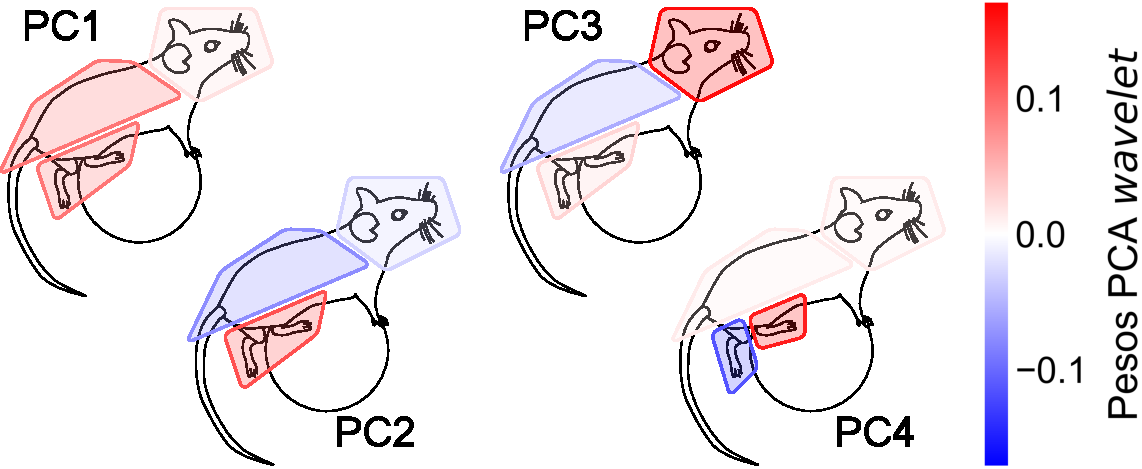
\includegraphics[width=0.8\linewidth]{figuras/capitulo4/partes_del_cuerpo_pca.pdf}
    \caption{\textbf{Pictograma de diferentes modos de locomoción.}
        Ilustración de cómo contribuyen diferentes partes del cuerpo a las 4 primeras componentes principales (PCs) de los espectros \textit{wavelet}. La PC1 consiste en movimientos de todas las partes del cuerpo en proporciones iguales, excepto por la menor participación de la cabeza. La PC2 tiene contribuciones opuestas en los movimientos de las patas respecto de la espalda-cola-nariz. La PC3 está dominada principalmente por movimientos de la cabeza. La PC4 es una locomoción con asimetría entre las patas traseras izquierda y derecha. Para más información sobre los pesos PCA ver \autoref{fig:capitulo4_pesos_pca}}
    \label{fig:capitulo4_partes_del_cuerpo_pca}
\end{figure}

Específicamente, se construyeron 2 mapas UMAP utilizando 2 conjuntos de características comportamentales diferentes. Esto se hizo con la intención de comparar las propiedades de representaciones comportamentales obtenidas a partir de la medición de diferentes aspectos del comportamiento animal. En particular, uno de los mapas se construyó a partir de las primeras 50 componentes principales (Figuras \ref{fig:capitulo4_partes_del_cuerpo_pca} y \ref{sec:apendice_pca_wavelet}) de los espectros \textit{wavelet} de los movimientos de los ángulos entre partes del cuerpo de los ratones, las cuales capturan el 84\% de la varianza de los datos. Esto se hizo para facilitar el cómputo de la proyección UMAP: el cálculo de UMAP a partir de 50 componentes principales puede realizarse en una computadora personal, mientras que el cálculo de UMAP a partir de las 500 variables que describen los espectros \textit{wavelet} requiere mayor memoria.

Por su parte, el segundo mapa UMAP se construyó a partir de las características que describen los pasos y las poses de los ratones (\autoref{fig:capitulo4_caracteristicas_pasos_poses}). Adicionalmente, las características de los pasos se promediaron entre las patas izquierda y derecha de los ratones, para eliminar diferencias por pata dominante de los ratones, mientras que las características de las poses, es decir, las posiciones de los marcadores de las partes del cuerpo, se procesaron para eliminar también diferencias por lateralidad en los ratones. Más en detalle: se relativizaron las posiciones de los marcadores respecto al centro de masa de los ratones y se calculó el valor absoluto de sus coordenadas horizontales; similarmente, la coordenada horizontal del centro de masa de los ratones se relativizó al centro del compartimento del rotarod donde se ubica el ratón, y se calculó su valor absoluto; y, finalmente, las coordenadas de las patas izquierda y derecha se reemplazaron por nuevas variables calculadas a partir de la diferencia y el promedio en las posiciones de las patas. De esta manera, se quitó efectivamente toda distinción entre izquierda y derecha en las características, volviendo indistinguibles ratones diestros de zurdos. Esto se hizo porque en el análisis no supervisado de comportamiento que se realizó anteriormente, en el trabajo de licenciatura, se observaron diferencias entre individuos asociadas a su lateralidad.

Debido a la complejidad en memoria del algoritmo UMAP, el cómputo de los mapas debe hacerse sobre una muestra parcial del conjunto de datos. Para cada conjunto de características se tomaron muestras aleatorias de datos con la misma densidad de probabilidad que la densidad de pasos ejecutados por el ratón en el tiempo. Es decir, los intervalos de tiempo en los que el ratón dio una mayor cantidad de pasos fueron muestreados con mayor frecuencia que otros intervalos de tiempo, de igual duración, pero con un menor número de pasos registrados. Esto se hizo para representar mejor la actividad del ratón, siguiendo la escala de tiempo natural de su comportamiento: los tiempos de sus pasos.

En resumen, el mapa UMAP de las componentes principales de los espectros \textit{wavelet} (\autoref{fig:capitulo4_umap_wav}) se construyó con 255\,060 puntos (4.7\% del total) y el mapa UMAP de las características de pasos y poses (\autoref{fig:capitulo4_umap_stp}) se construyó con 509\,995 puntos (9.3\% del total). Ambos mapas se construyeron usando similaridad coseno como noción de distancia en el espacio original de los datos, y con parámetros del \textit{kernel} de densidad en el espacio de dimensión baja $a=1.0$ y $b=0.4$. El mapa UMAP \textit{wavelet} se construyó con $n_{\mathrm{neighbors}}=100$ y el mapa de pasos y poses con $n_{\mathrm{neighbors}}=30$. Se utilizó un mayor número de vecinos cercanos en el mapa \textit{wavelet} para compensar por el mayor tiempo de autocorrelación de estas características, y permitir que se formen relaciones de similaridad entre los datos por fuera de su autocorrelación temporal (\autoref{fig:capitulo4_componentes_pca}). Esto no fue necesario para el mapa de pasos y poses, donde se usó el número de vecinos por defecto, ya que estas características tienen menores tiempos de autocorrelación (\autoref{fig:capitulo4_caracteristicas_pasos_poses}). Finalmente, para mapear el resto de los puntos que no fueron muestreados al construir las proyecciones UMAP se utilizó un clasificador $k$-NN (\textit{k-Nearest Neighbors}) con $k=5$ vecinos cercanos. De esta manera, se obtuvieron las proyecciones UMAP de 5\,458\,552 puntos en total, representando cada uno de estos un instante de tiempo de un ratón ejecutando una prueba rotarod en particular.

\section{Estructura espacial y temporal de los mapas}\label{sec:umap_trans}

Para obtener categorías que aglutinen comportamientos similares (\textit{labels}) se realizaron segmentaciones \textit{watershed} de los mapas UMAP. Este algoritmo no requiere que se defina \textit{a priori} un número fijo de regiones a encontrar. El espacio UMAP está formado por picos y valles de densidad de puntos. La segmentación \textit{watershed} encuentra áreas conexas del mapa que encierren estos picos de densidad de puntos y estén separadas entre sí por los valles de baja densidad \cite{meyer_watershed_history, compact}. Para obtener esta segmetanción se calcularon las densidades de probabilidad de los puntos en los mapas UMAP usando \texttt{fastKDE}, una herramienta para estimación rápida de densidad de probabilidad implementada en Python \cite{obrien_fastkde}, mientras que la segmentación \textit{watershed} se realizó con el paquete \texttt{scikit-image} \cite{scikit-image}. Se utilizó este algoritmo de segmentación por su eficiencia computacional para procesar conjuntos de datos bidimensionales de millones de puntos. Al terminar este proceso se obtuvieron 10 \textit{labels} de comportamiento para cada mapa. Los parámetros del algoritmo de segmentación se pueden ajustar para realizar particiones más finas o más gruesas del mapa. En nuestro caso decidimos mantener el número de regiones encontradas entre 5 y 20 para facilitar el análisis, por lo que afinamos los parámetros del algoritmo para este fin. De hecho, existen otros algoritmos de segmentación, por ejemplo HDBSCAN (\textit{Hierarchical Density-Based Spatial Clustering of Applications with Noise}), que permiten obtener segmentaciones en categorías jerarquizadas con diferentes niveles de detalle \cite{hdbscan}. Sin embargo, la eficiencia computacional de la simple segmentación \textit{watershed} fue más conveniente. Para poder utilizar una herramienta de segmentación jerárquica como HDBSCAN es necesario trabajar con una muestra de alrededor de 100\,000 datos o menos, debido a su complejidad computacional en memoria.

\begin{figure}[htbp]
    \centering
    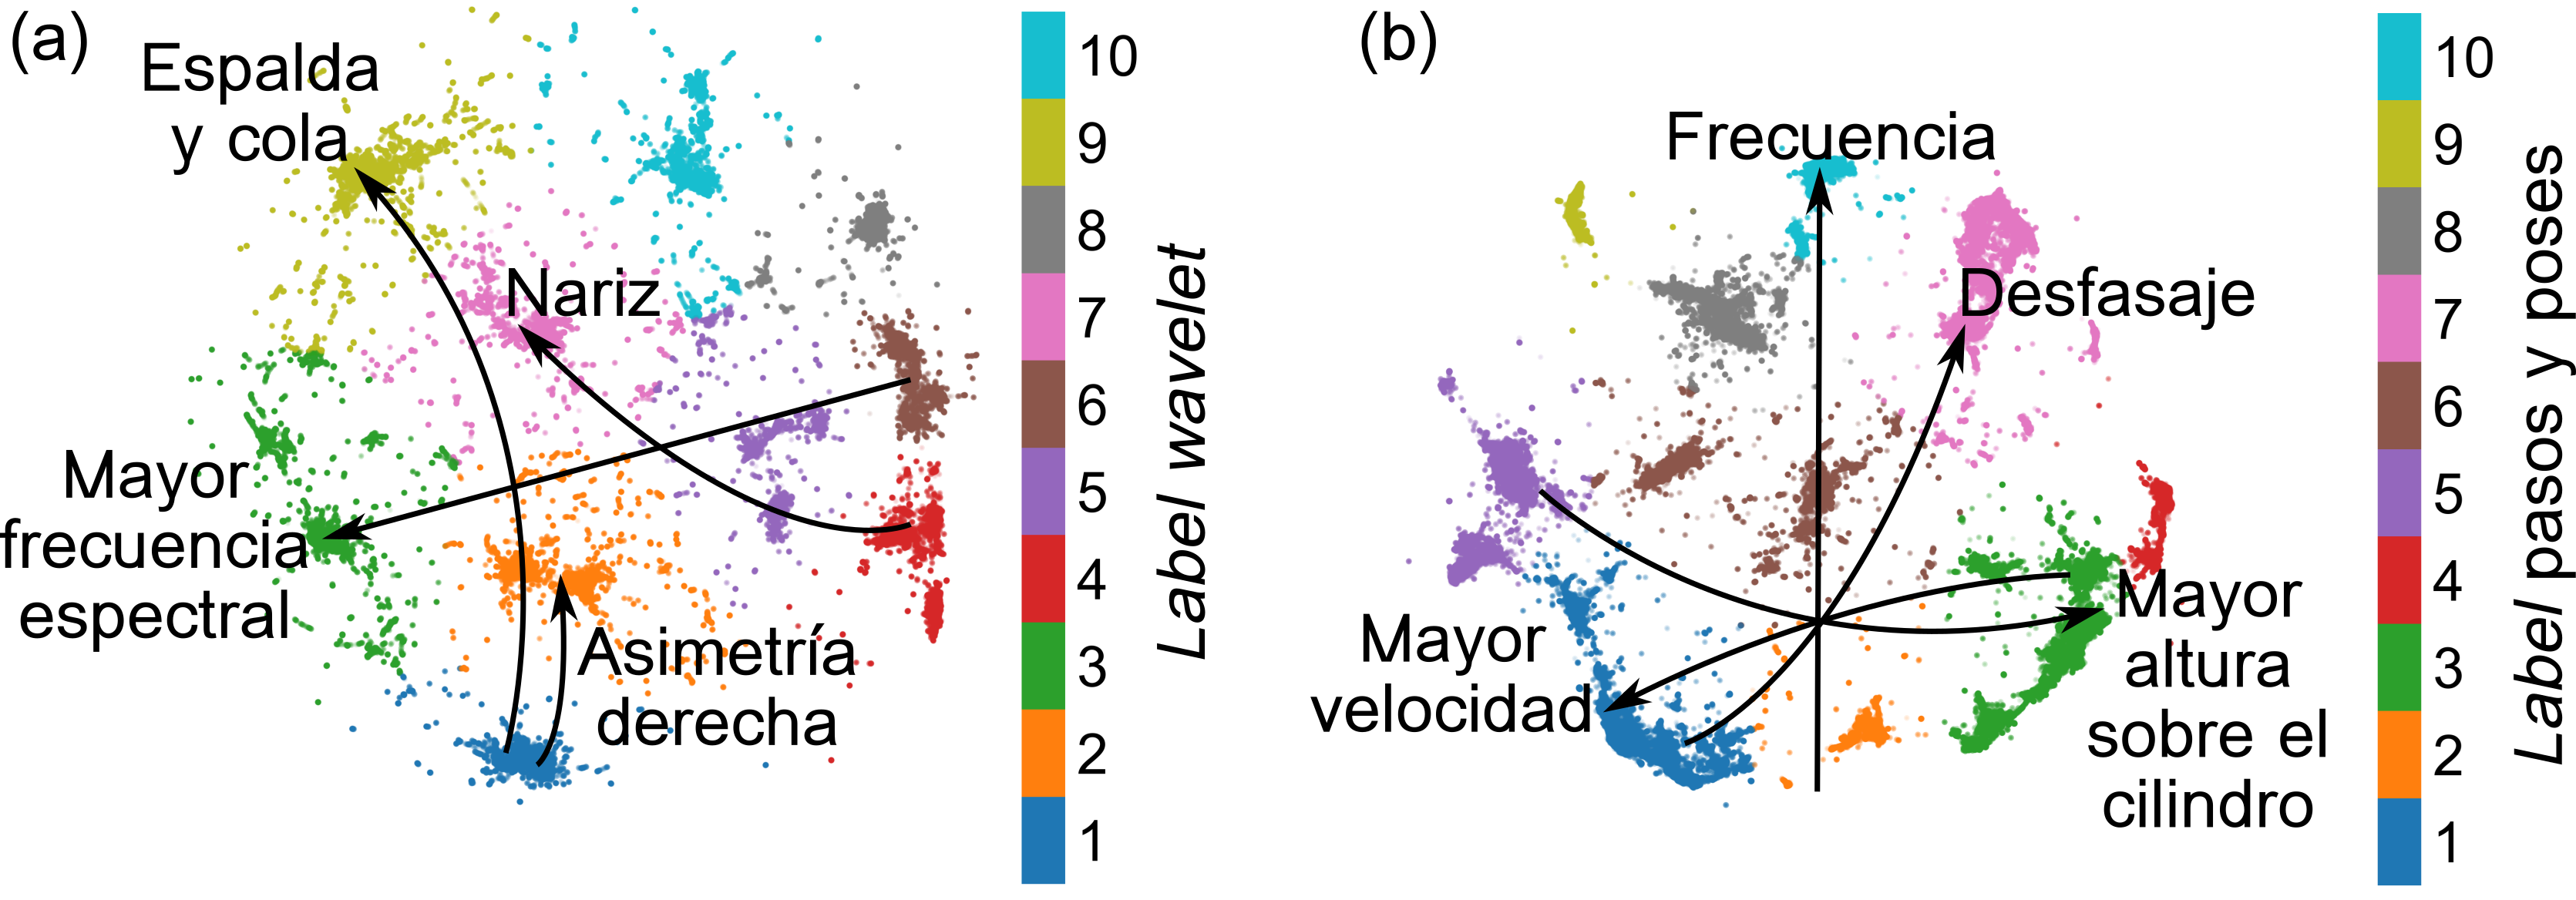
\includegraphics[width=0.99\linewidth]{figuras/capitulo4/comentario_label_umap.png}
    \caption{\textbf{Descripción de las propiedades de los comportamientos de cada mapa.}
        Las flechas indican, de manera simplificada, el sentido en que aumentan diferentes propiedades sobre el mapa. (a) Proyección UMAP de las primeras 50 componentes principales de los espectros \textit{wavelet} de partes del cuerpo del ratón. Se observan regiones en el mapa con diferente frecuencia promedio espectral, y diferencias en los movimientos de la espalda-cola, nariz y asimetría entre patas traseras derecha e izquierda. (b) Proyección UMAP de las características de pasos y poses. Se observan regiones del mapa con diferentes frecuencias de pasos, desfasajes, velocidades y alturas a las que el ratón se posiciona sobre el cilindro.}
    \label{fig:capitulo4_comentario_label_umap}
\end{figure}

Ocasionalmente, estos métodos no supervisados de clasificación pueden resultar en categorías de comportamiento difíciles de reconocer por parte de un humano o de describir en pocas palabras \cite{datta_computational_neuroethology, berman_mapping}. Esto suele ocurrir más frecuentemente en las representaciones de comportamientos complejos. De todas formas, podemos intentar describir en términos generales algunos aspectos de cada label (\autoref{fig:capitulo4_comentario_label_umap} obtenida a partir del análisis de las Figuras \ref{fig:capitulo4_umap_wav} y \ref{fig:capitulo4_umap_stp} suplementarias). Por ejemplo en el mapa UMAP \textit{wavelet} (\autoref{fig:capitulo4_comentario_label_umap}a), podemos observar que los \textit{labels} 4, 5, 6, 8 y 10 tienen menores valores de la primera componente principal (PC1, en la \autoref{fig:capitulo4_umap_wav}a) de los espectros \textit{wavelet} que los \textit{labels} 1, 2, 3, 7 y 9. La PC1, a su vez, acompaña a la frecuencia espectral promedio del movimiento de todas las partes del cuerpo (\autoref{fig:capitulo4_partes_del_cuerpo_pca}), por lo que está asociada a qué tan rápido se mueven las partes del cuerpo de los ratones. Haciendo un análisis similar, y observando los valores de la segunda componente principal (\autoref{fig:capitulo4_umap_wav}b), deducimos que el \textit{label} 9 está asociado a un tipo de locomoción con mucho movimiento en la espalda y en la cola, relativo al movimiento de las patas traseras, mientras que para el \textit{label} 1 se observa la situación opuesta. Usando la tercera componente principal (\autoref{fig:capitulo4_umap_wav}c), asociamos al \textit{label} 7 con locomoción con mucho movimiento de la nariz y la cabeza del animal. Finalmente, el \textit{label} 2 está asociado a un mayor movimiento de la pata trasera derecha que la izquierda, y se observa lo opuesto para el \textit{label} 1, mientras que para el resto de \textit{labels} la asimetría es menos perceptible (\autoref{fig:capitulo4_umap_wav}d).
Por su parte, en el mapa UMAP de pasos y poses (\autoref{fig:capitulo4_comentario_label_umap}b), observamos que los \textit{labels} 3, 4, 7 y 10 corresponden a estrategias donde los pasos de las patas traseras se realizan a una altura elevada sobre el cilindro rotarod, mientras que los \textit{labels} 1, 5 están asociados a pasos en la parte más baja del cilindro (\autoref{fig:capitulo4_umap_stp}a). Respecto a las velocidades promedio de los pasos (\autoref{fig:capitulo4_umap_stp}b), los \textit{labels} 2, 3, 4 y 10, junto con una parte del 6 y del 7, son de baja velocidad de pasos, mientras que los \textit{labels} 1, 5 y 8, junto con la otra parte del 6 y del 7, son de mayor velocidad de pasos. En cuanto al desfasaje entre las patas traseras (\autoref{fig:capitulo4_umap_stp}c), el \textit{label} 7 está asociado a pasos con gran desfasaje y los \textit{labels} 1 y 3 presentan parcialmente puntos con bajo desfasaje. Quizá la relación más clara sea la de la frecuencia con la que el ratón da pasos (\autoref{fig:capitulo4_umap_stp}d), la cual aumenta gradualmente desde abajo hacia arriba en el espacio UMAP, siendo los \textit{labels} 1, 2, 3 y 4 los de menor frecuencia y los \textit{labels} 9 y 10 de mayor frecuencia.

Una de las razones por las que realizamos dos proyecciones UMAP a partir de diferentes conjuntos de características para describir el comportamiento es para estudiar qué tanta información tienen en común ambas representaciones. Ya que no siempre es claro qué características comportamentales son más relevantes o informativas \textit{a priori} y muchas veces se identifican características inesperadas potencialmente útiles de esta manera. Una vez obtenidos los \textit{labels} de comportamiento en el UMAP \textit{wavelet} y en el UMAP pasos y poses, calculamos el valor de la información mutua ajustada entre las dos segmentaciones de datos, usando la implementación en Python de \texttt{scikit-learn} \texttt{metrics.adjusted\_mutual\_info\_score} \cite{scikit-learn, adjusted_mutual_info_score}. Esta es una medida de qué tan similares son ambas maneras de categorizar el comportamiento de los ratones. Este valor puede estar entre 0 y 1, con 0 correspondiendo a segmentaciones completamente independientes entre sí (es decir, cada una aportaría información nueva sobre el comportamiento) y con 1 correspondiendo a segmentaciones equivalentes desde el punto de vista de la información nueva que aportan. En nuestro caso, la información mutua ajustada entre las segmentaciones es de 0.22, el cual es un valor relativamente bajo, pero no insignificante. Esto quiere decir que las dos maneras propuestas para representar el comportamiento animal aportan información novedosa entre sí. Esto tiene sentido, pues los espectros \textit{wavelet} de los ángulos de las partes del cuerpo de los ratones aportan información principalmente sobre la dinámica de sus movimientos, mientras que las características de los pasos y las poses de los ratones aportan mayormente información sobre las posiciones de sus partes del cuerpo en el espacio en un dado instante.

Esto da paso a la pregunta, ¿qué pasaría si combinamos las características dinámicas de los \textit{wavelets} con las características de los pasos y poses en una misma representación del comportamiento? Nuestra hipótesis es que un tipo de características dominará sobre el resto en la representación. Esto se debe, por un lado, a que las proyecciones UMAP tienen que comprometer ciertos aspectos de los datos para poder representarlos en solo dos dimensiones, y, por otro lado, en el momento en que realizamos una segmentación \textit{watershed} de los mapas estamos eligiendo un nivel de detalle en nuestros \textit{labels}. Esto obligaría a que se priorice un tipo de características comportamentales por sobre las demás, mientras que el resto de características podrían influir en la estructura más fina y detallada de los mapas comportamentales. Esta sería una situación interesante para aplicar una segmentación jerárquica, por ejemplo HDBSCAN, para tener acceso a representaciones más finas del comportamiento y conocer su ordenamiento. Sin embargo, esto también haría que el análisis sea mucho más complejo, pasando por diferentes escalas de detalle. De todas formas, en este trabajo se realizó una especie de prueba piloto al combinar varios tipos de características en una proyección UMAP: las características de pasos y poses. Un análisis de información mutua de los \textit{labels} de pasos y poses con sus características correspondientes revela que un tipo de característica (específicamente los valores en los eventos de pasos) aporta mucha más información acerca de estos \textit{labels} que las demás variables (\autoref{fig:capitulo4_mi_labels_scaler_stp}). Esto apoya nuestra hipótesis de que al usar varios tipos de características heterogéneas, alguno de estos tipos termina dominando sobre los demás, por lo menos al usar un nivel de detalle similar al presentado en nuestro análisis.

Otra cuestión interesante es investigar la estructura temporal de los \textit{labels} obtenidos. Por ejemplo, ver qué \textit{labels} se utilizan más comúnmente al iniciar y al terminar una prueba rotarod. Dado que los \textit{labels} tienen duraciones variables (Figuras \ref{fig:capitulo4_labels_umap_wav}c y \ref{fig:capitulo4_labels_umap_stp}c), el estudio de su probabilidad de ocurrencia, sin corregir por su duración, podría traer como consecuencia una sobre-representación de los \textit{labels} que duren más en cada una de sus apariciones. Para reducir estas diferencias debido a la variabilidad de las duraciones, definimos secuencias condensadas de \textit{labels} agrupándolos en bloques consecutivos de una misma categoría comportamental y considerando cada uno de estos bloques como una única observación del \textit{label}. De esta manera resultan secuencias de \textit{labels} sin repeticiones consecutivas de una misma categoría de comportamiento, para las que reservaremos la denominación de ``secuencias'', para diferenciarlas de las ``series temporales'' de \textit{labels} de donde provienen. Con estas secuencias de \textit{labels}, sin repeticiones consecutivas, construimos los grafos de transiciones temporales de cada mapa UMAP (Figuras \ref{fig:capitulo4_labels_umap_wav}b y \ref{fig:capitulo4_labels_umap_stp}b). Adicionalmente, utilizando los 5 primeros y 5 últimos \textit{labels} observados en las secuencias comportamentales de cada prueba calculamos las probabilidades de transiciones desde el estado ``inicio'' y hacia el estado ``fin'' de la prueba. Para cada mapa UMAP se observan conjuntos distintos de \textit{labels} que se observan con mayor frecuencia en el inicio o en el final de cada prueba rotarod. Al iniciar cada prueba, es más probable que un ratón ejecute los comportamientos 6, 8, 9 y 10 del mapa \textit{wavelets} (\autoref{fig:capitulo4_labels_umap_wav}b), o los comportamientos 1, 2, 3, 4 y 6 del mapa pasos y poses (\autoref{fig:capitulo4_labels_umap_stp}b). Mientras que antes de terminar una prueba, es más probable observar los comportamientos 1, 2 y 3 del mapa \textit{wavelets} (\autoref{fig:capitulo4_labels_umap_wav}b), o los comportamientos 1, 5, 6, 8 y 9 del mapa pasos y poses (\autoref{fig:capitulo4_labels_umap_stp}b).

Finalmente, nos preguntamos si la estructura espacial de las proyecciones UMAP tiene alguna relación con la estructura temporal de las secuencias de comportamientos. Esto puede observarse en primera instancia en los grafos de transiciones (Figuras \ref{fig:capitulo4_labels_umap_wav}b y \ref{fig:capitulo4_labels_umap_stp}b). Resulta que las transiciones temporales más probables se producen entre regiones colindantes en el mapa, tanto para el mapa \textit{wavelet} como para el mapa de pasos y poses. Más aún, se observa la existencia de una estructura espacial más fina si coloreamos los mapas UMAP según el \textit{label} que le sigue a cada punto en la secuencia de comportamiento (Figuras \ref{fig:capitulo4_labels_umap_wav}d y \ref{fig:capitulo4_labels_umap_stp}d). Efectivamente, dentro de cada región segmentada de los mapas se observan estructuras más finas donde hay una mayor preferencia por transiciones temporales hacia un tipo particular de \textit{label} por sobre los demás.

\begin{figure}[htbp]
    \centering
    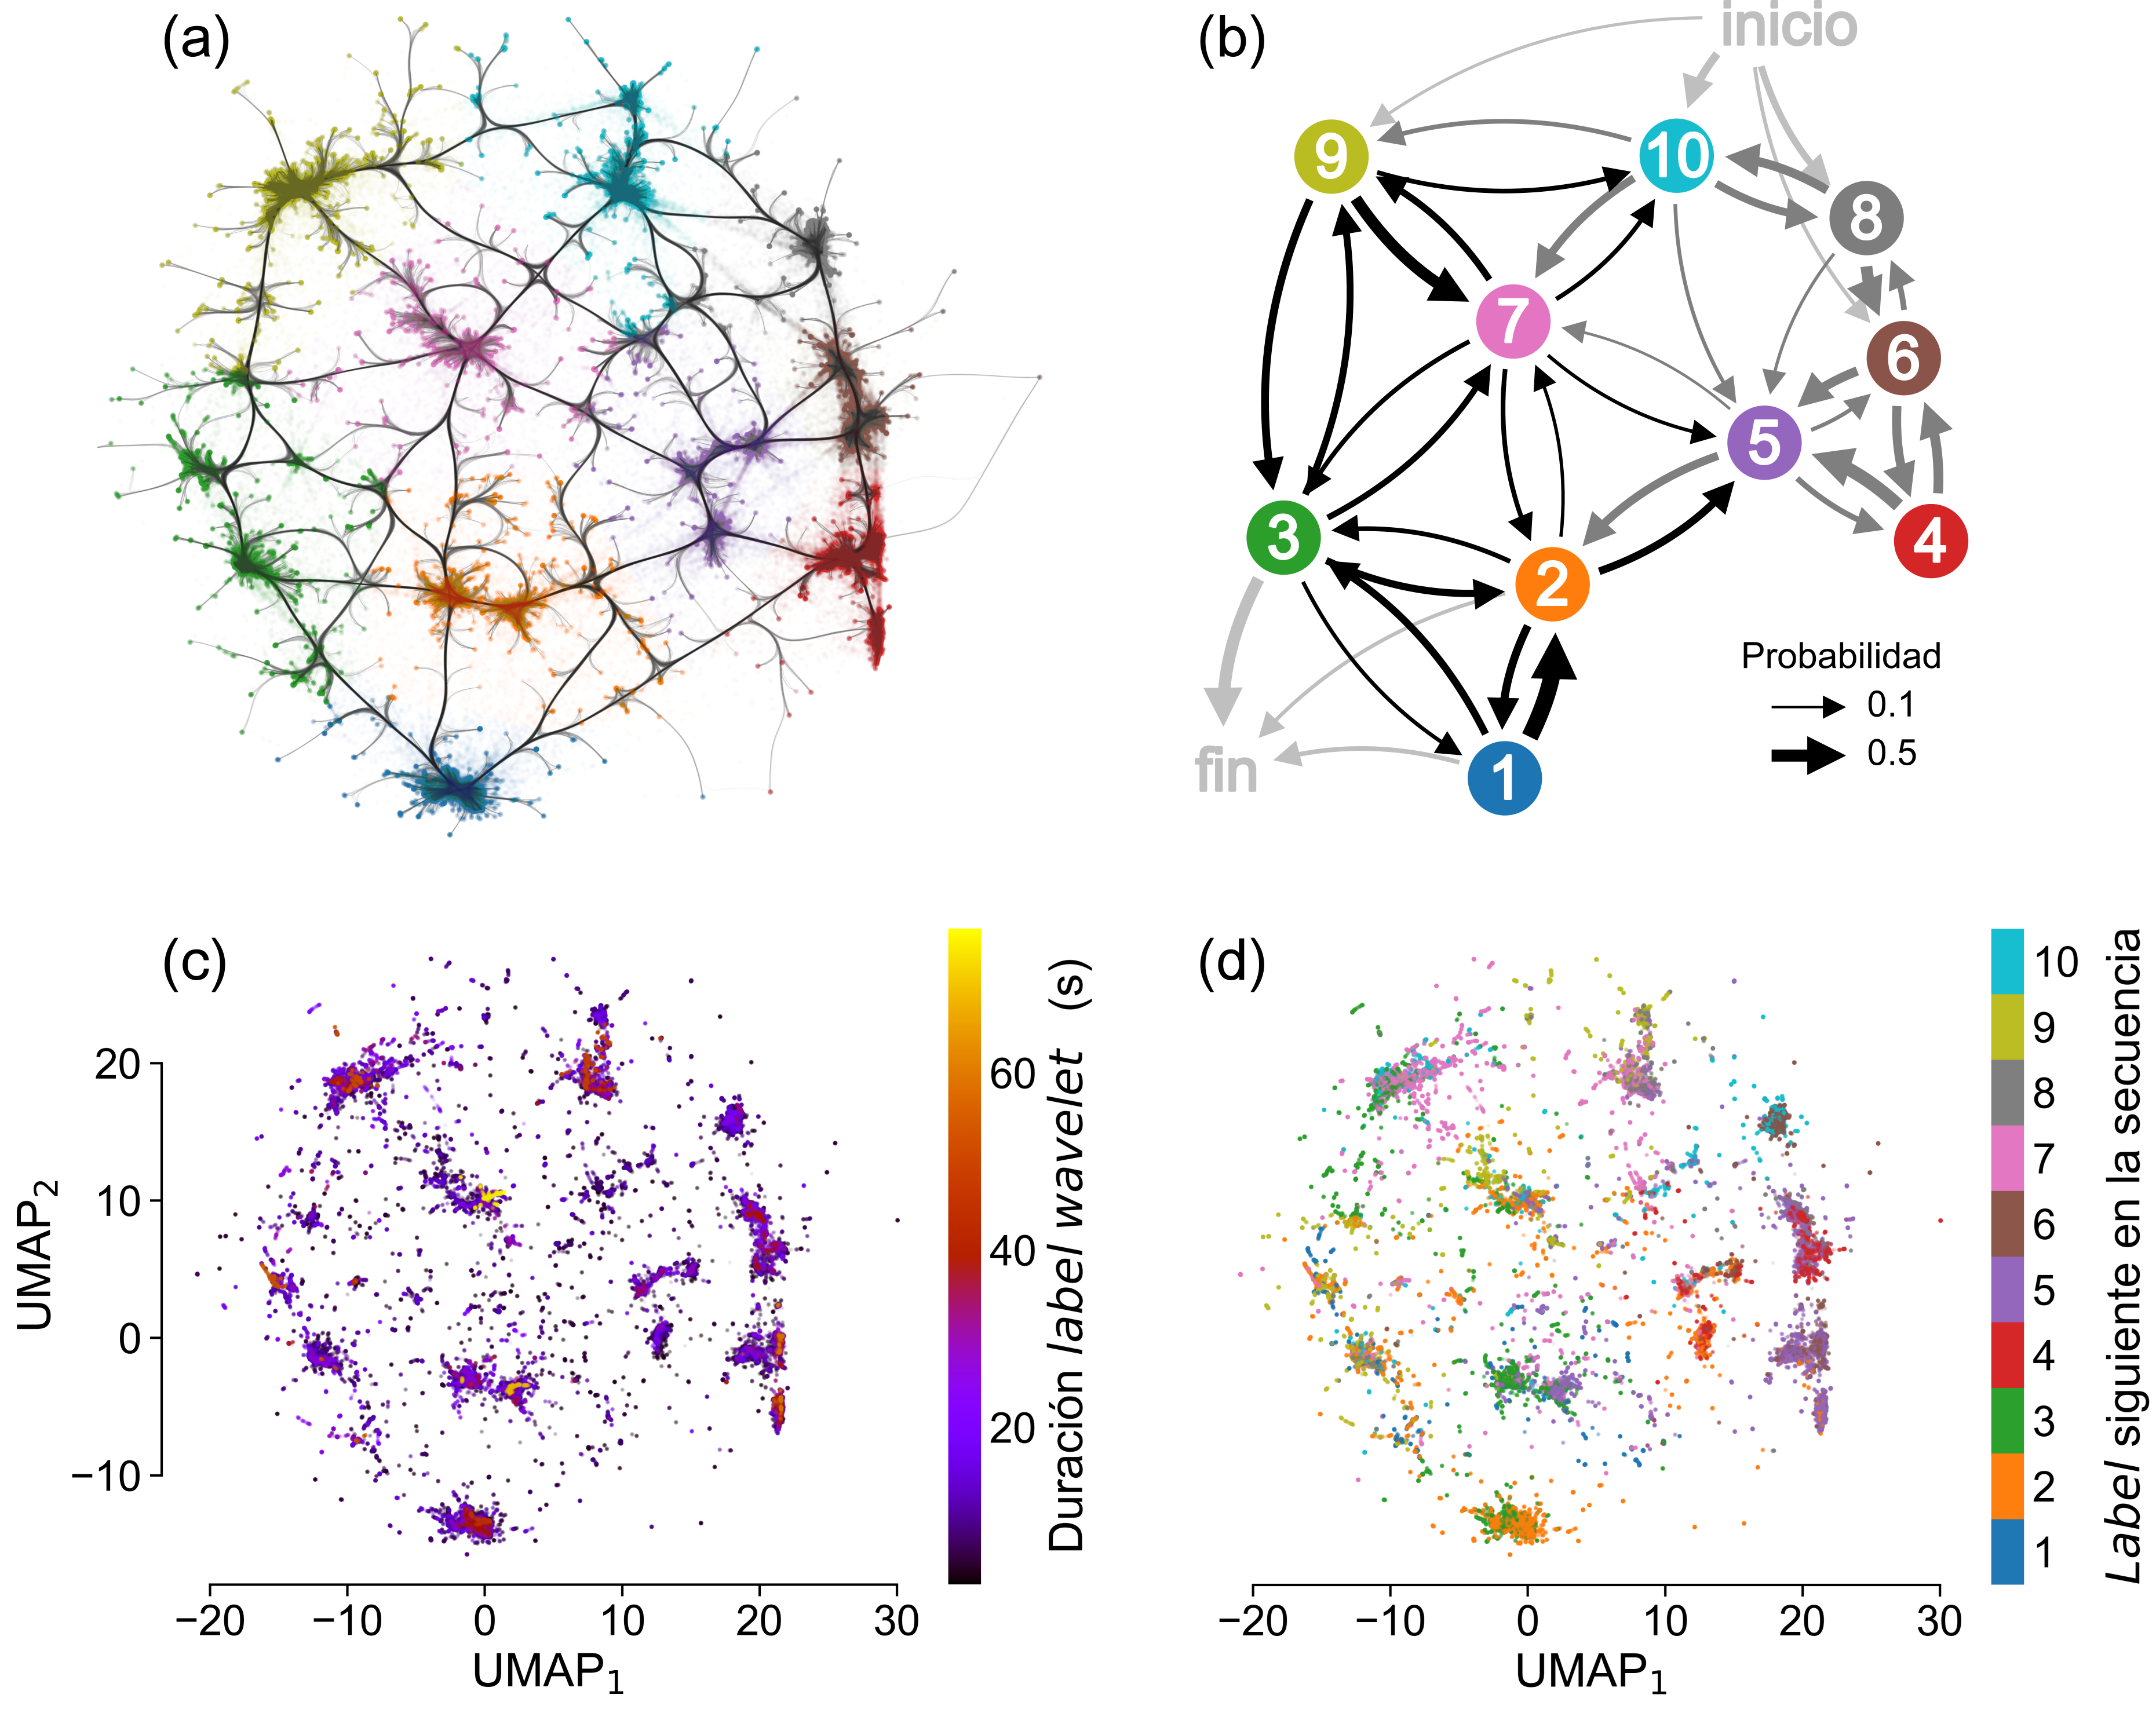
\includegraphics[width=0.99\linewidth]{figuras/capitulo4/labels_umap_wav.png}
    \caption{\textbf{\textit{Labels} de comportamiento de la proyección UMAP de las componentes principales de los espectros \textit{wavelet}.}
        (a) Similaridad entre los puntos del mapa. El grosor de cada línea es proporcional a la similaridad entre las características de las regiones conectadas. (b) Grafo de transiciones temporales de las secuencias de \textit{labels}. El grosor de las flechas es proporcional a la probabilidad de transición. Sólo se muestran transiciones con probabilidad mayor al 10\%. Las flechas oscuras (grises) son transiciones desde un \textit{label} con probabilidad marginal en la secuencia mayor al 10\%. Las probabilidades de transición desde el estado ``inicio'' y hacia el estado ``fin'' fueron calculados \textit{ad hoc}. (c) Duración de cada \textit{label} en la secuencia según su ubicación en el mapa. (d) Descripción más fina de las transiciones en la secuencia de \textit{labels} según de qué ubicación en el mapa provengan.}
    \label{fig:capitulo4_labels_umap_wav}
\end{figure}

\begin{figure}[htbp]
    \centering
    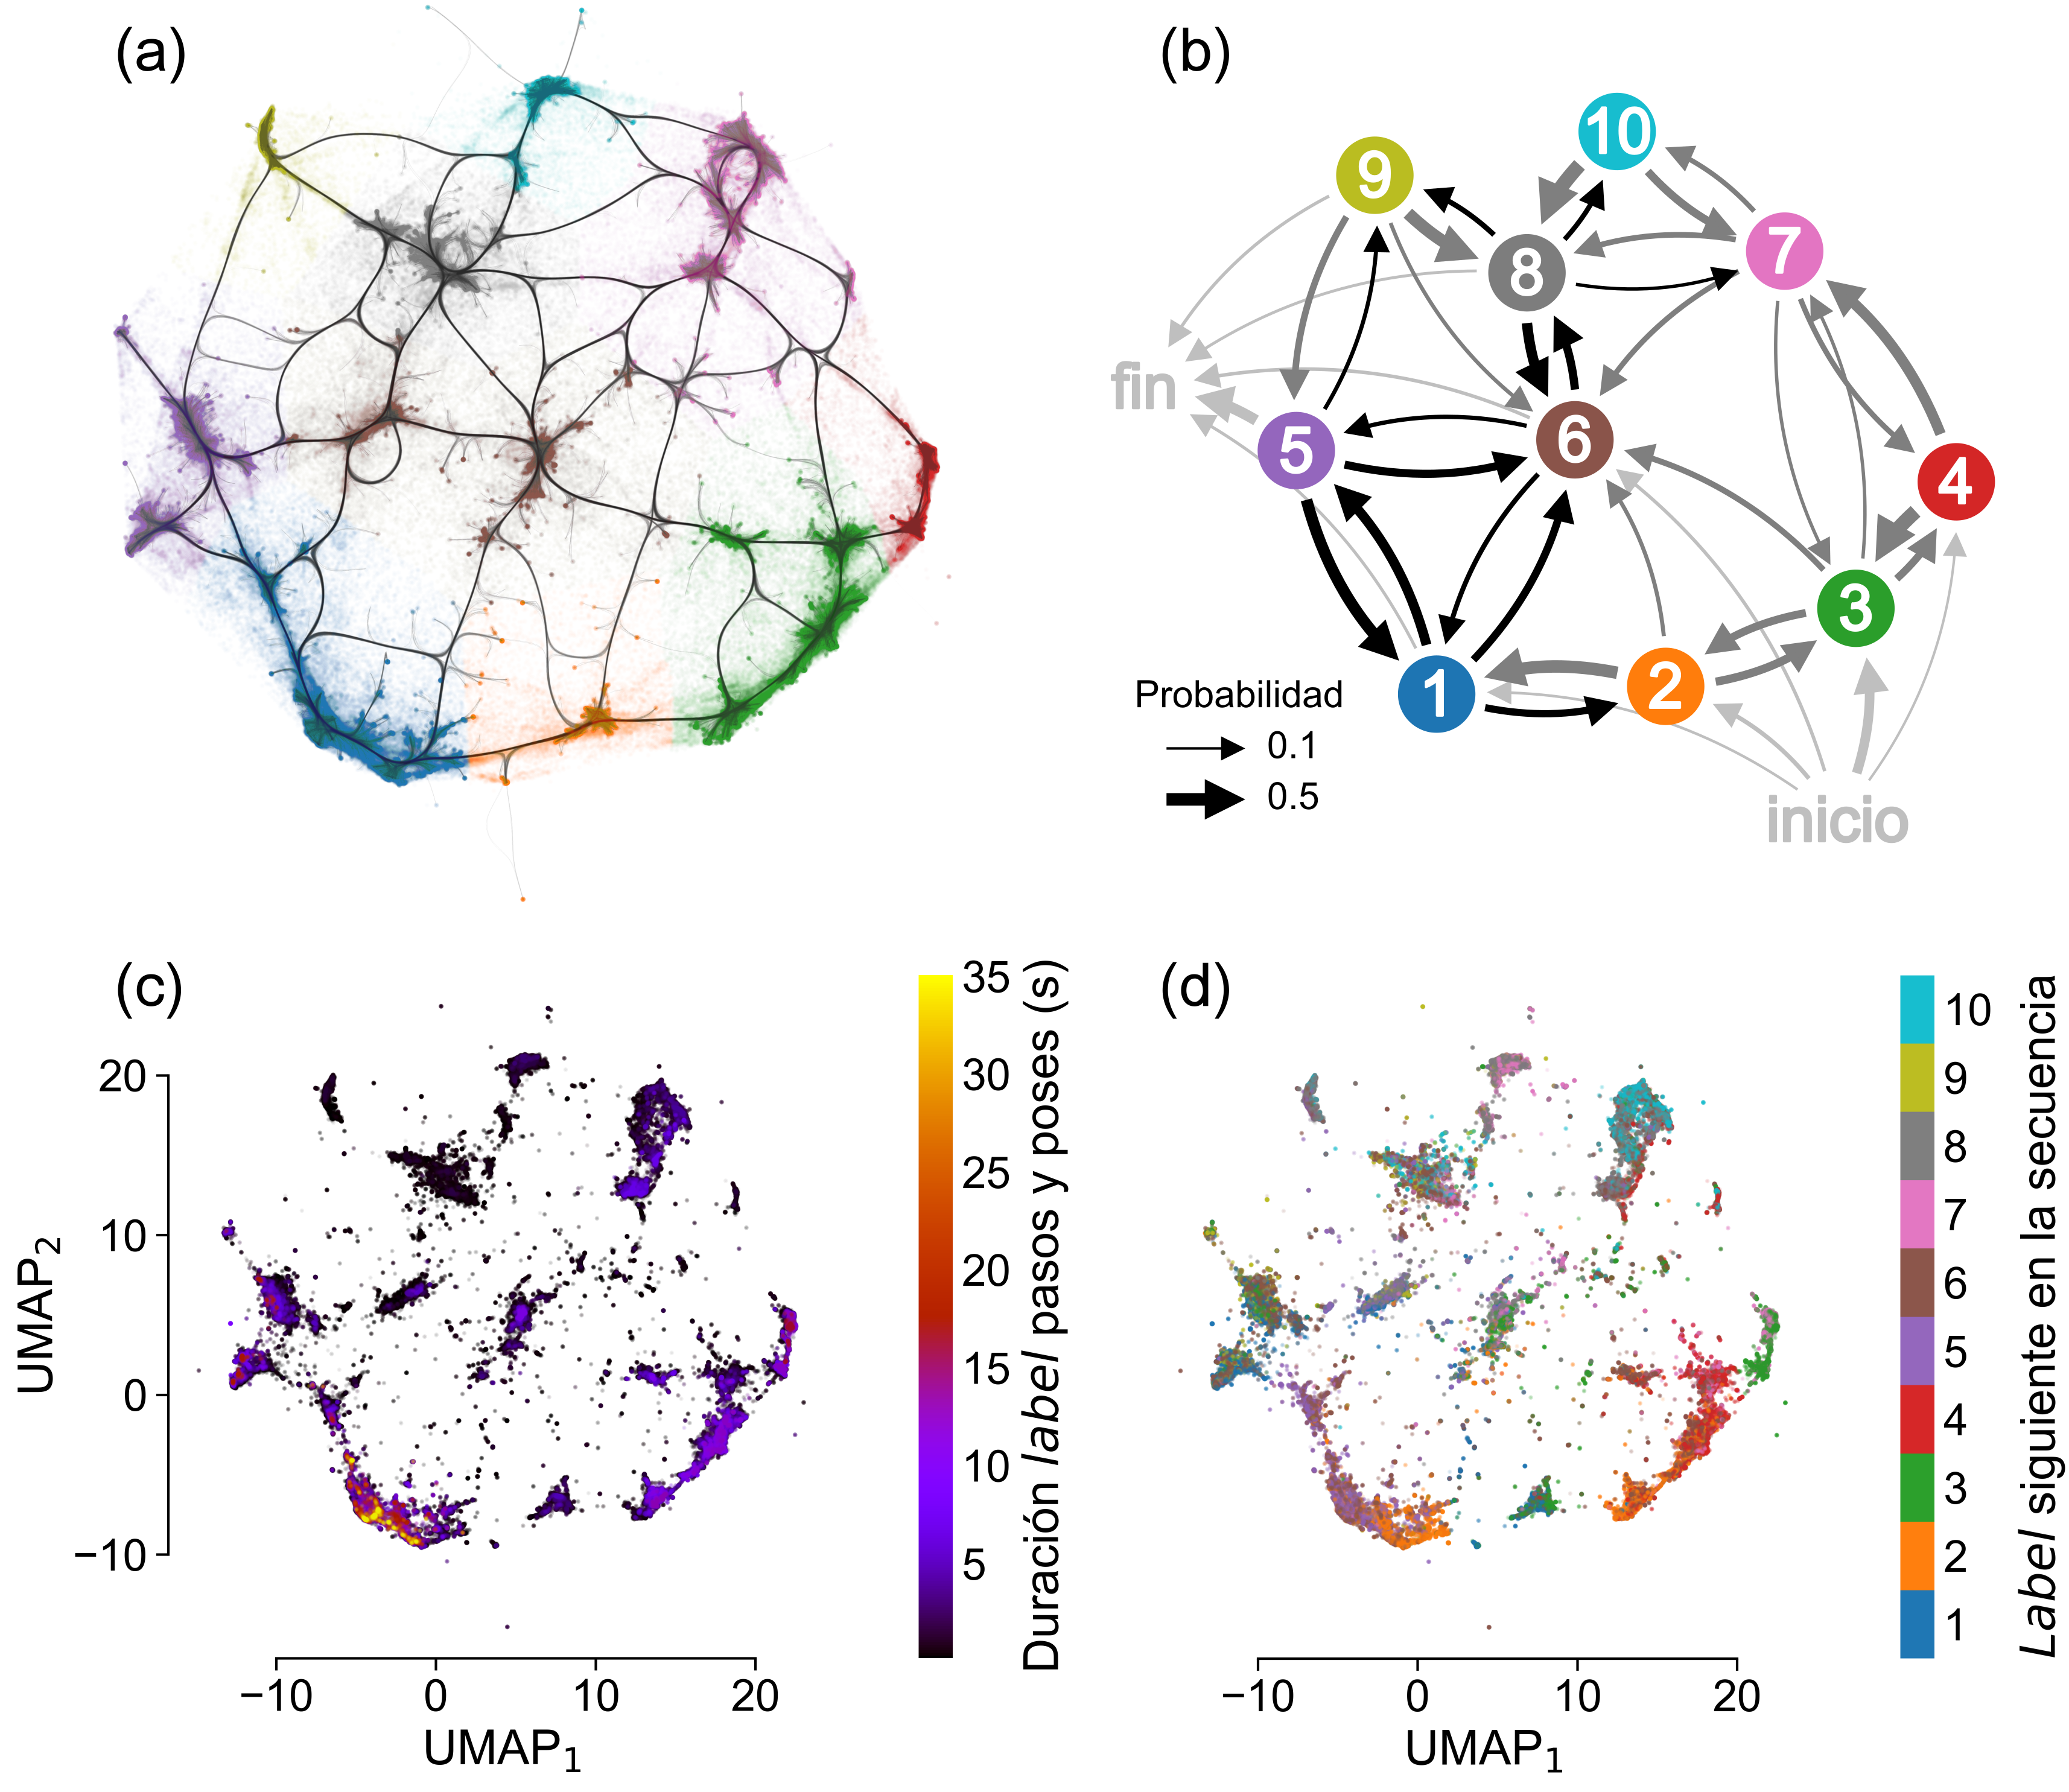
\includegraphics[width=0.99\linewidth]{figuras/capitulo4/labels_umap_stp.png}
    \caption{\textbf{\textit{Labels} de comportamiento de la proyección UMAP de las características de pasos y poses.}
        (a) Similaridad entre los puntos del mapa. El grosor de cada línea es proporcional a la similaridad entre las características de las regiones conectadas. (b) Grafo de transiciones temporales de las secuencias de \textit{labels}. El grosor de las flechas es proporcional a la probabilidad de transición. Sólo se muestran transiciones con probabilidad mayor al 10\%. Las flechas oscuras (grises) son transiciones desde un \textit{label} con probabilidad marginal en la secuencia mayor al 10\%. Las probabilidades de transición desde el estado ``inicio'' y hacia el estado ``fin'' fueron calculados \textit{ad hoc}. (c) Duración de cada \textit{label} en la secuencia según su ubicación en el mapa. (d) Descripción más fina de las transiciones en la secuencia de \textit{labels} según de qué ubicación en el mapa provengan.}
    \label{fig:capitulo4_labels_umap_stp}
\end{figure}

\clearpage

\section{Cambios en las secuencias de comportamiento}\label{sec:probabilidad_labels}

En principio, cada uno de los 10 ratones estudiados puede acceder, en un determinado instante de una prueba rotarod, a cualquiera de los estados comportamentales presentes en los mapas. Sin embargo, en la práctica los comportamientos representados en el mapa no son exhibidos por todos los individuos de la misma manera, y a su vez los repertorios comportamentales de cada individuo varían a lo largo del entrenamiento (Figuras \ref{fig:capitulo4_probabilidades_labels_wav} y \ref{fig:capitulo4_probabilidades_labels_stp}). En general, se observa que los \textit{labels} de pasos y poses separan más marcadamente a los ratones entre los grupos de alto y bajo rendimiento, comparados con los \textit{labels} \textit{wavelet}. Esto se debe a que las diferencias entre grupos de rendimiento aparecen como una estructura fina en la segmentación \textit{watershed} del mapa UMAP \textit{wavelet} (\autoref{fig:capitulo4_umap_wav}g). En otras palabras, los grupos de rendimiento están más mezclados de manera global en el mapa UMAP \textit{wavelet}, aunque pueden recuperarse las diferencias entre grupos si se accede a un nivel de detalle más fino. Mientras que en el mapa UMAP de pasos y poses hay una separación clara entre los grupos de rendimiento que fue mayormente capturada por la segmentación \textit{watershed} \textit{wavelet} (\autoref{fig:capitulo4_umap_stp}g). A grandes rasgos, esto indica que la dinámica global del movimiento de las partes del cuerpo de los ratones (espectros \textit{wavelet}) no es muy diferente entre grupos de rendimiento; mientras que en términos globales, las posiciones de las partes del cuerpo de los ratones en el cilindro y las características de sus pasos presentan diferencias más marcadas en comparación.

Para estudiar comportamientos bajo condiciones experimentales similares entre pruebas, analizamos la probabilidad de ocurrencia de \textit{labels} en los primeros 100 s de secuencias de comportamiento de cada prueba rotarod realizada. De esta manera, en el mapa UMAP \textit{wavelet}, los \textit{labels} 2 y 5 son exhibidos más frecuentemente por los ratones de bajo rendimiento y los \textit{labels} 9 y 10 por los de alto rendimiento. El resto, los \textit{labels} 1, 3, 4, 5, 6, 7, y 8 no son utilizados exclusivamente por ningún grupo de rendimiento (\autoref{fig:capitulo4_probabilidades_labels_wav}). Por su parte, en el mapa UMAP de pasos y poses, la diferencia entre grupos de rendimiento se manifiesta más fuertemente en la probabilidad de los \textit{labels} de comportamiento durante los primeros 100 s de las pruebas rotarod. Los \textit{labels} 1, 2, 5 y 6 son exhibidos preferentemente por los ratones de bajo rendimiento, mientras que los \textit{labels} 3, 4 y 7 son utilizados principalmente por los ratones de alto rendimiento. Solamente los \textit{labels} 8, 9 y 10 son utilizados en proporciones similares por ambos grupos de rendimiento (\autoref{fig:capitulo4_probabilidades_labels_stp}). De acuerdo a la interpretación del mapa de pasos y poses de la \autoref{fig:capitulo4_comentario_label_umap}b, los ratones de bajo rendimiento tienden a dar pasos de mayor velocidad, presentan menor desfasaje entre sus patas traseras (o sea que las levantan más o menos al mismo tiempo), se mueven a alturas más bajas sobre el cilindro y dan pasos a menor frecuencia (o sea que dejan pasar más tiempo entre pasos consecutivos y son arrastrados una distancia mayor por la rotación del cilindro). En comparación, los ratones de alto rendimiento dan pasos más cortos a menor velocidad, manteniéndose en la parte superior del cilindro la mayor parte del tiempo, con tendencia a un mayor desfasaje entre sus pasos (es decir, tienen una locomoción más alternante). Muchas de las probabilidades de \textit{label} en la secuencia varían significativamente a lo largo de los días de entrenamiento, a juzgar por los p-valores de test \textit{one-way} ANOVA (Figuras \ref{fig:capitulo4_probabilidades_labels_wav} y \ref{fig:capitulo4_probabilidades_labels_stp}). En muchos casos se observa además una gran variabilidad intra-día en las probabilidades de \textit{label} en los primeros 100 s de las secuencias de comportamiento. En consecuencia, la gran variabilidad intra-día reduce la significancia estadística de la variación de estas métricas durante el entrenamiento, especialmente para el grupo de 3 ratones de alto rendimiento comparado con el grupo de 7 ratones de bajo rendimiento. A pesar de esto, se observa en términos generales una reducción en la variabilidad intra-día de las probabilidades de los \textit{labels}, indicando que con el entrenamiento se afianza la ejecución de ciertos tipos de comportamiento con mayor precisión.

En resumen, se observa una estructura temporal en las secuencias de labels, existiendo una marcada preferencia por iniciar y terminar las pruebas rotarod usando categorías de comportamientos diferentes. Los \textit{labels} de pasos y poses separan más fuertemente a los ratones según su grupo de rendimiento, comparados con los \textit{labels} \textit{wavelet}. Esto puede deberse a que los espectros wavelets presentan más invarianzas, matemáticamente hablando, que las características de pasos y poses. Específicamente, los espectros wavelet de los ángulos de las partes del cuerpo de los ratones son invariantes ante pequeñas rotaciones rígidas, traslaciones espacio-temporales y cambios de escala en el cuerpo de los ratones, por lo que tiene sentido que separen menos a los ratones individualmente al ser características que generalizan mejor.

Se observa que la variabilidad en las probabilidades de labels durante los primeros 100 s de las secuencias de comportamiento se reduce con el entrenamiento. Esto se observa a través de la entropía de las secuencias (\autoref{fig:capitulo4_entropia}), la cual se reduce significativamente para ambos grupos de rendimiento en el caso de los \textit{labels wavelet} (\autoref{fig:capitulo4_entropia}a) y significativamente para los 7 ratones de bajo rendimiento en los \textit{labels} de pasos y poses (\autoref{fig:capitulo4_entropia}b). Para ambos tipos de \textit{labels} no se observan diferencias significativas entre los grupos de rendimiento en los valores de las entropías. Sin embargo, la entropía de los comportamientos de los 3 ratones de alto rendimiento es ligeramente inferior durante todo el entrenamiento. La entropía de las proyecciones UMAP también se reduce con los días de entrenamiento (Figuras \ref{fig:capitulo4_umap_wav}h y \ref{fig:capitulo4_umap_stp}h suplementarias). Sosteniendo que la variabilidad en las estrategias de comportamiento usadas por los ratones se reduce con el aprendizaje. El uso de mapas UMAP de dimensión reducida permite un enfoque holístico en el estudio del comportamiento: permite estudiar los efectos y cambios de múltiples características comportamentales simultáneamente en una conveniente representación de fácil visualización.

\begin{figure}[htbp]
    \centering
    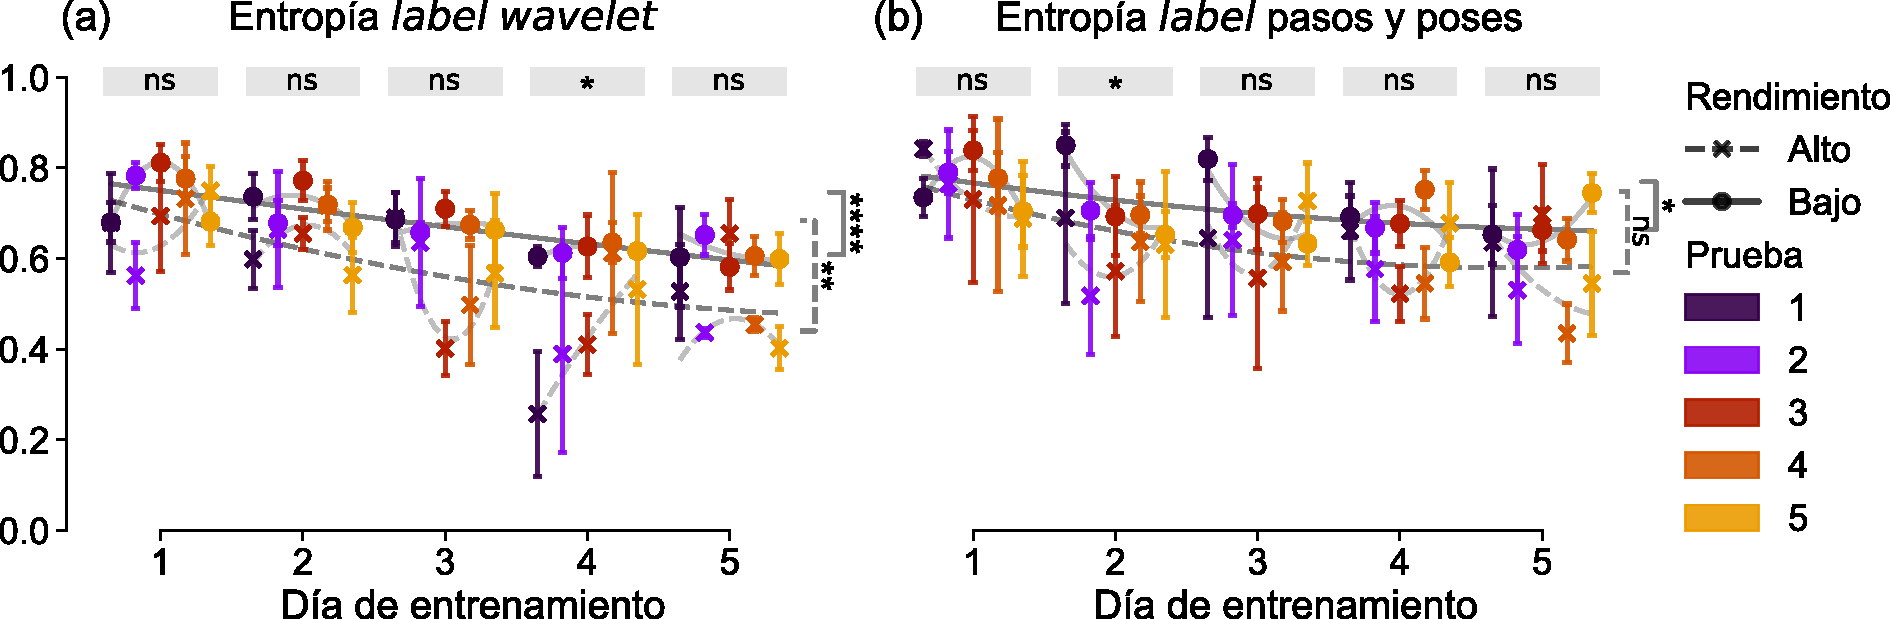
\includegraphics[width=0.99\linewidth]{figuras/capitulo4/entropia.pdf}
    \caption{\textbf{Entropía de las secuencias de \textit{labels}.}
        Entropía de las secuencias de comportamientos durante los primeros 100 s de las pruebas rotarod, para cada día de entrenamiento y número de prueba realizada ese día. Las entropías son relativas a la entropía máxima dada por la distribución marginal de los \textit{labels} en las secuencias. Los puntos muestran el promedio por grupo de rendimiento y las barras son el error estándar del promedio. Los rectángulos grises, en el margen superior de cada subfigura, indican los p-valores T-test entre grupos de rendimiento para cada día. Los corchetes en los márgenes derechos indican, para cada grupo de rendimiento, los p-valores \textit{one-way} ANOVA agrupando por día de entrenamiento. (a) \textit{Labels wavelet}. (b) \textit{Labels} pasos y poses.}
    \label{fig:capitulo4_entropia}
\end{figure}

\begin{figure}[htbp]
    \centering
    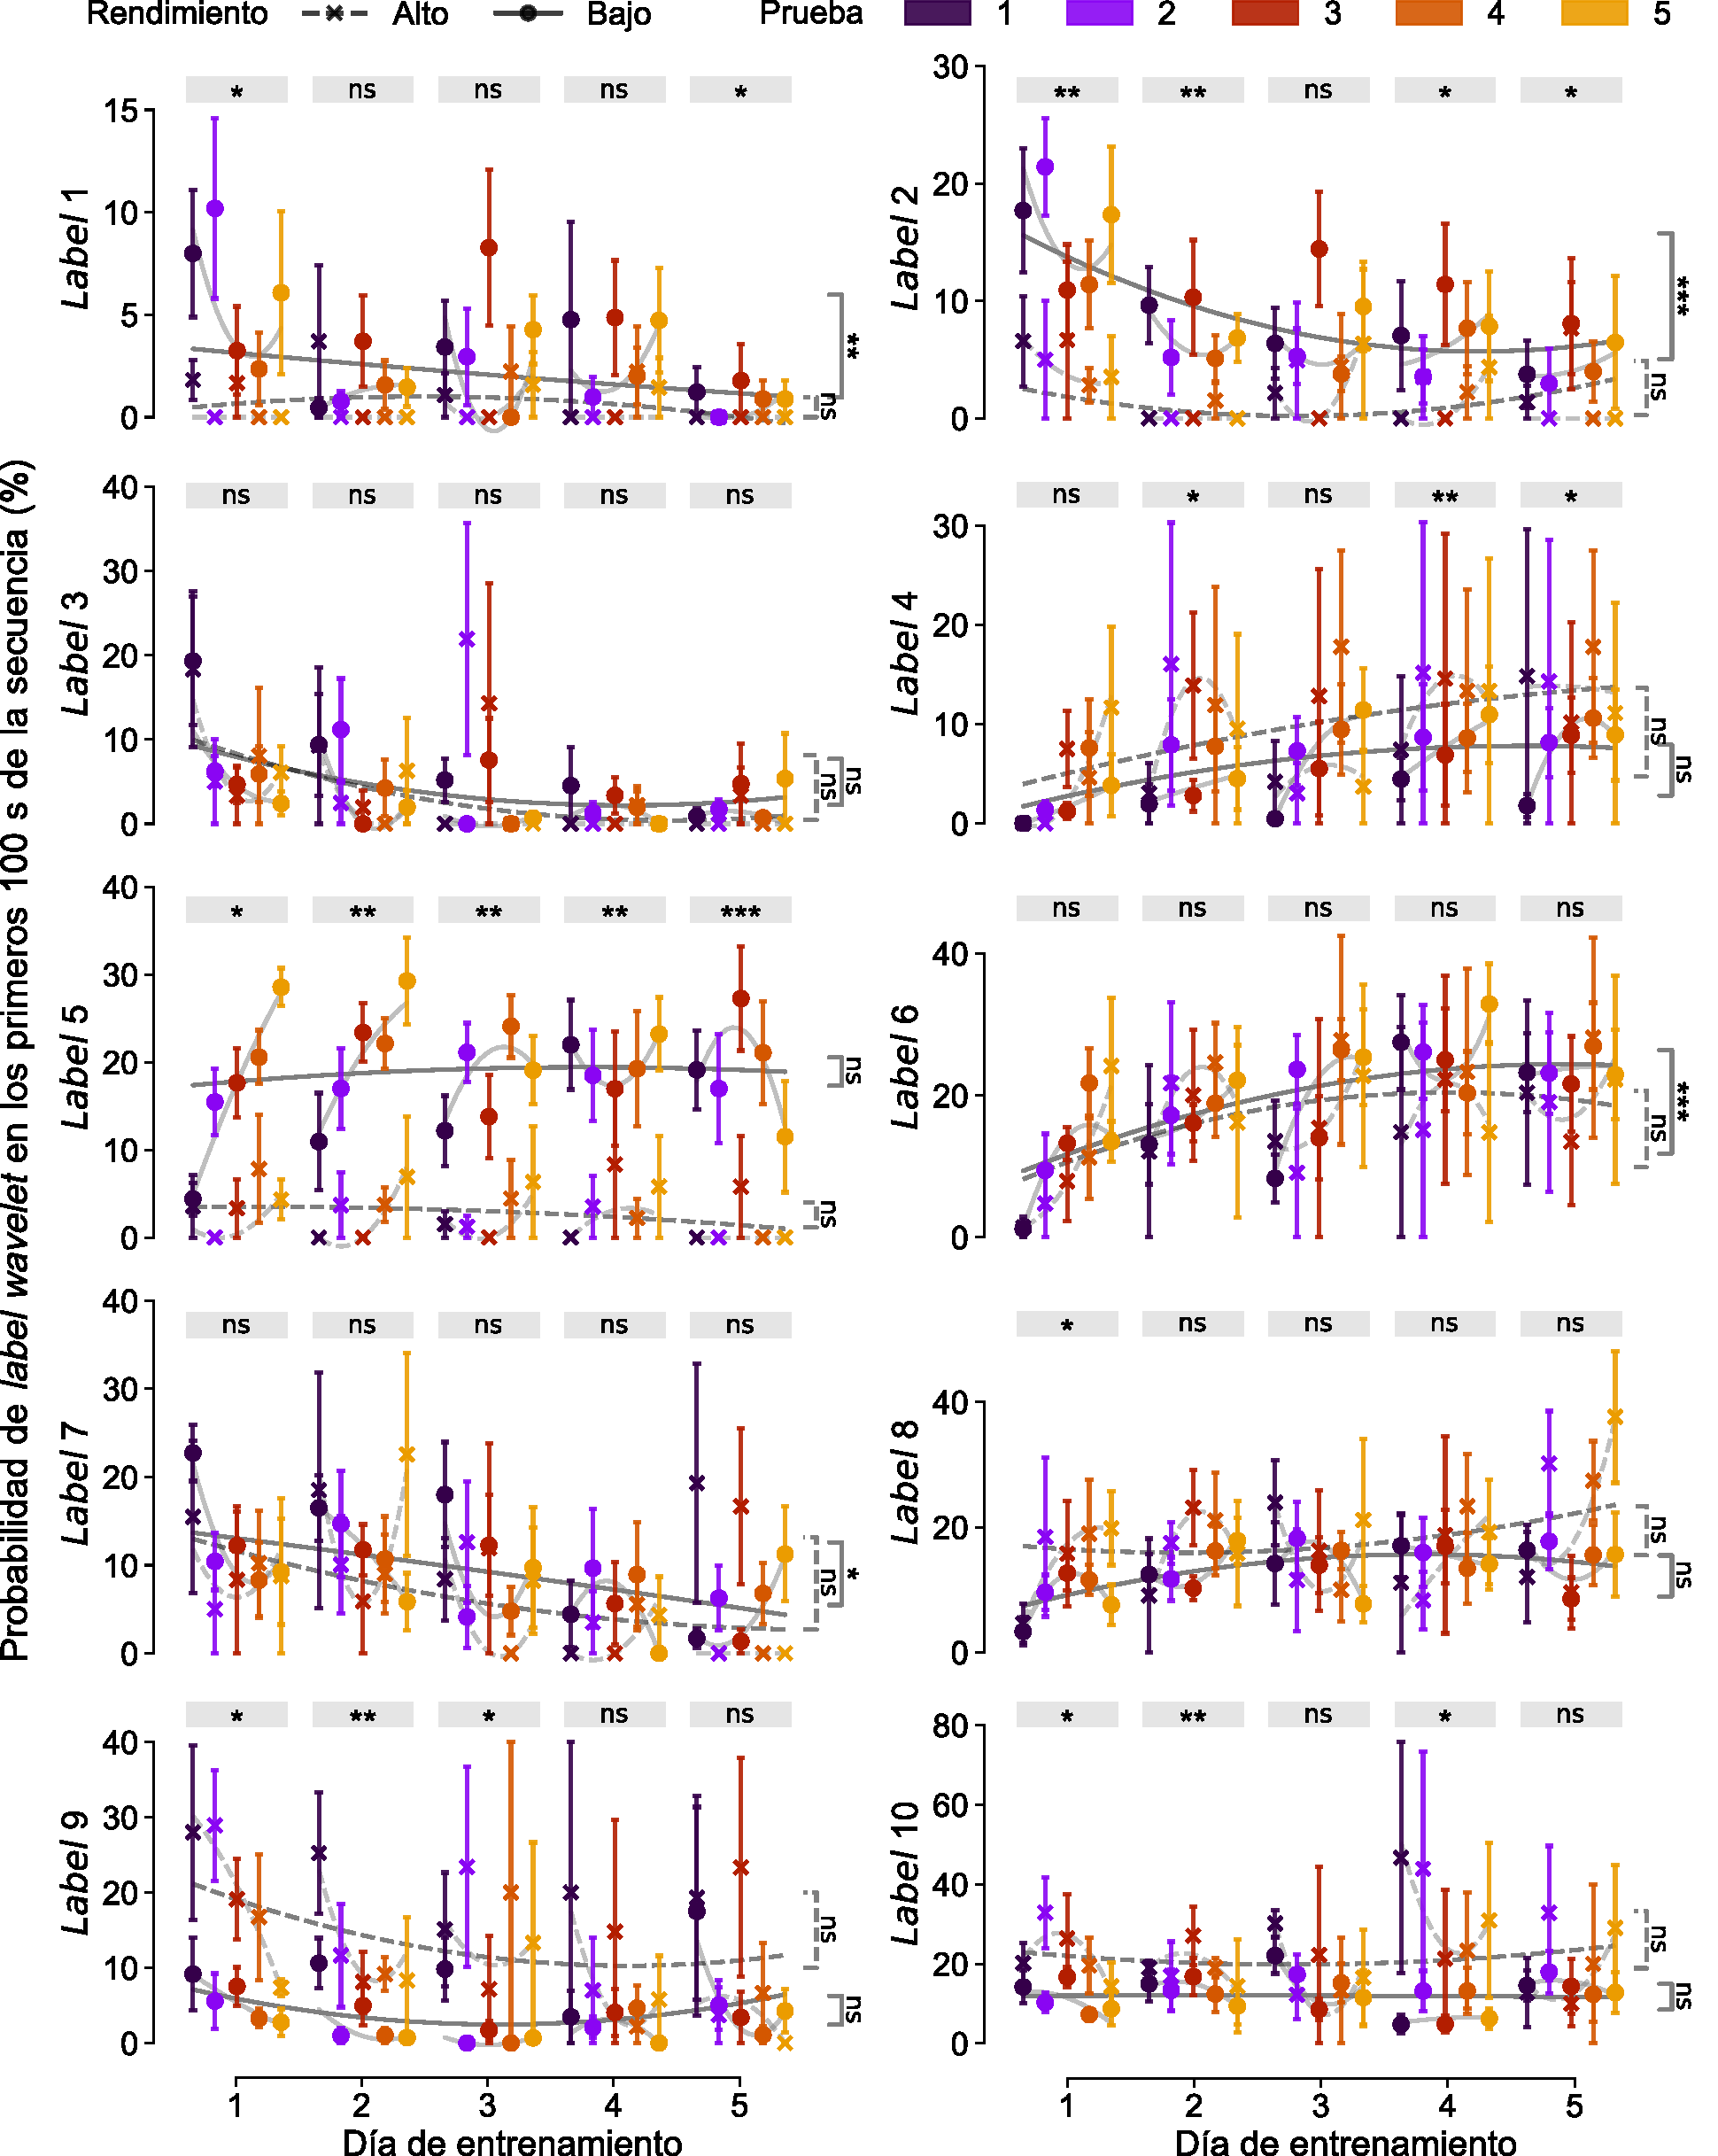
\includegraphics[width=0.99\linewidth]{figuras/capitulo4/probabilidades_labels_wav.pdf}
    \caption{\textbf{Cambios en las probabilidades de \textit{label} \textit{wavelet} en las secuencias de comportamiento.} Cada subfigura de la grilla representa la probabilidad de ocurrencia de un determinado \textit{label} durante los primeros 100 s de las pruebas rotarod, para cada día de entrenamiento y número de prueba realizada ese día. Los puntos muestran el promedio por grupo de rendimiento y las barras son el error estándar del promedio. Los rectángulos grises, en el margen superior de cada subfigura, indican los p-valores T-test entre grupos de rendimiento para cada día. Los corchetes en los márgenes derechos indican, para cada grupo de rendimiento, los p-valores \textit{one-way} ANOVA agrupando por día de entrenamiento.}
    \label{fig:capitulo4_probabilidades_labels_wav}
\end{figure}

\begin{figure}[htbp]
    \centering
    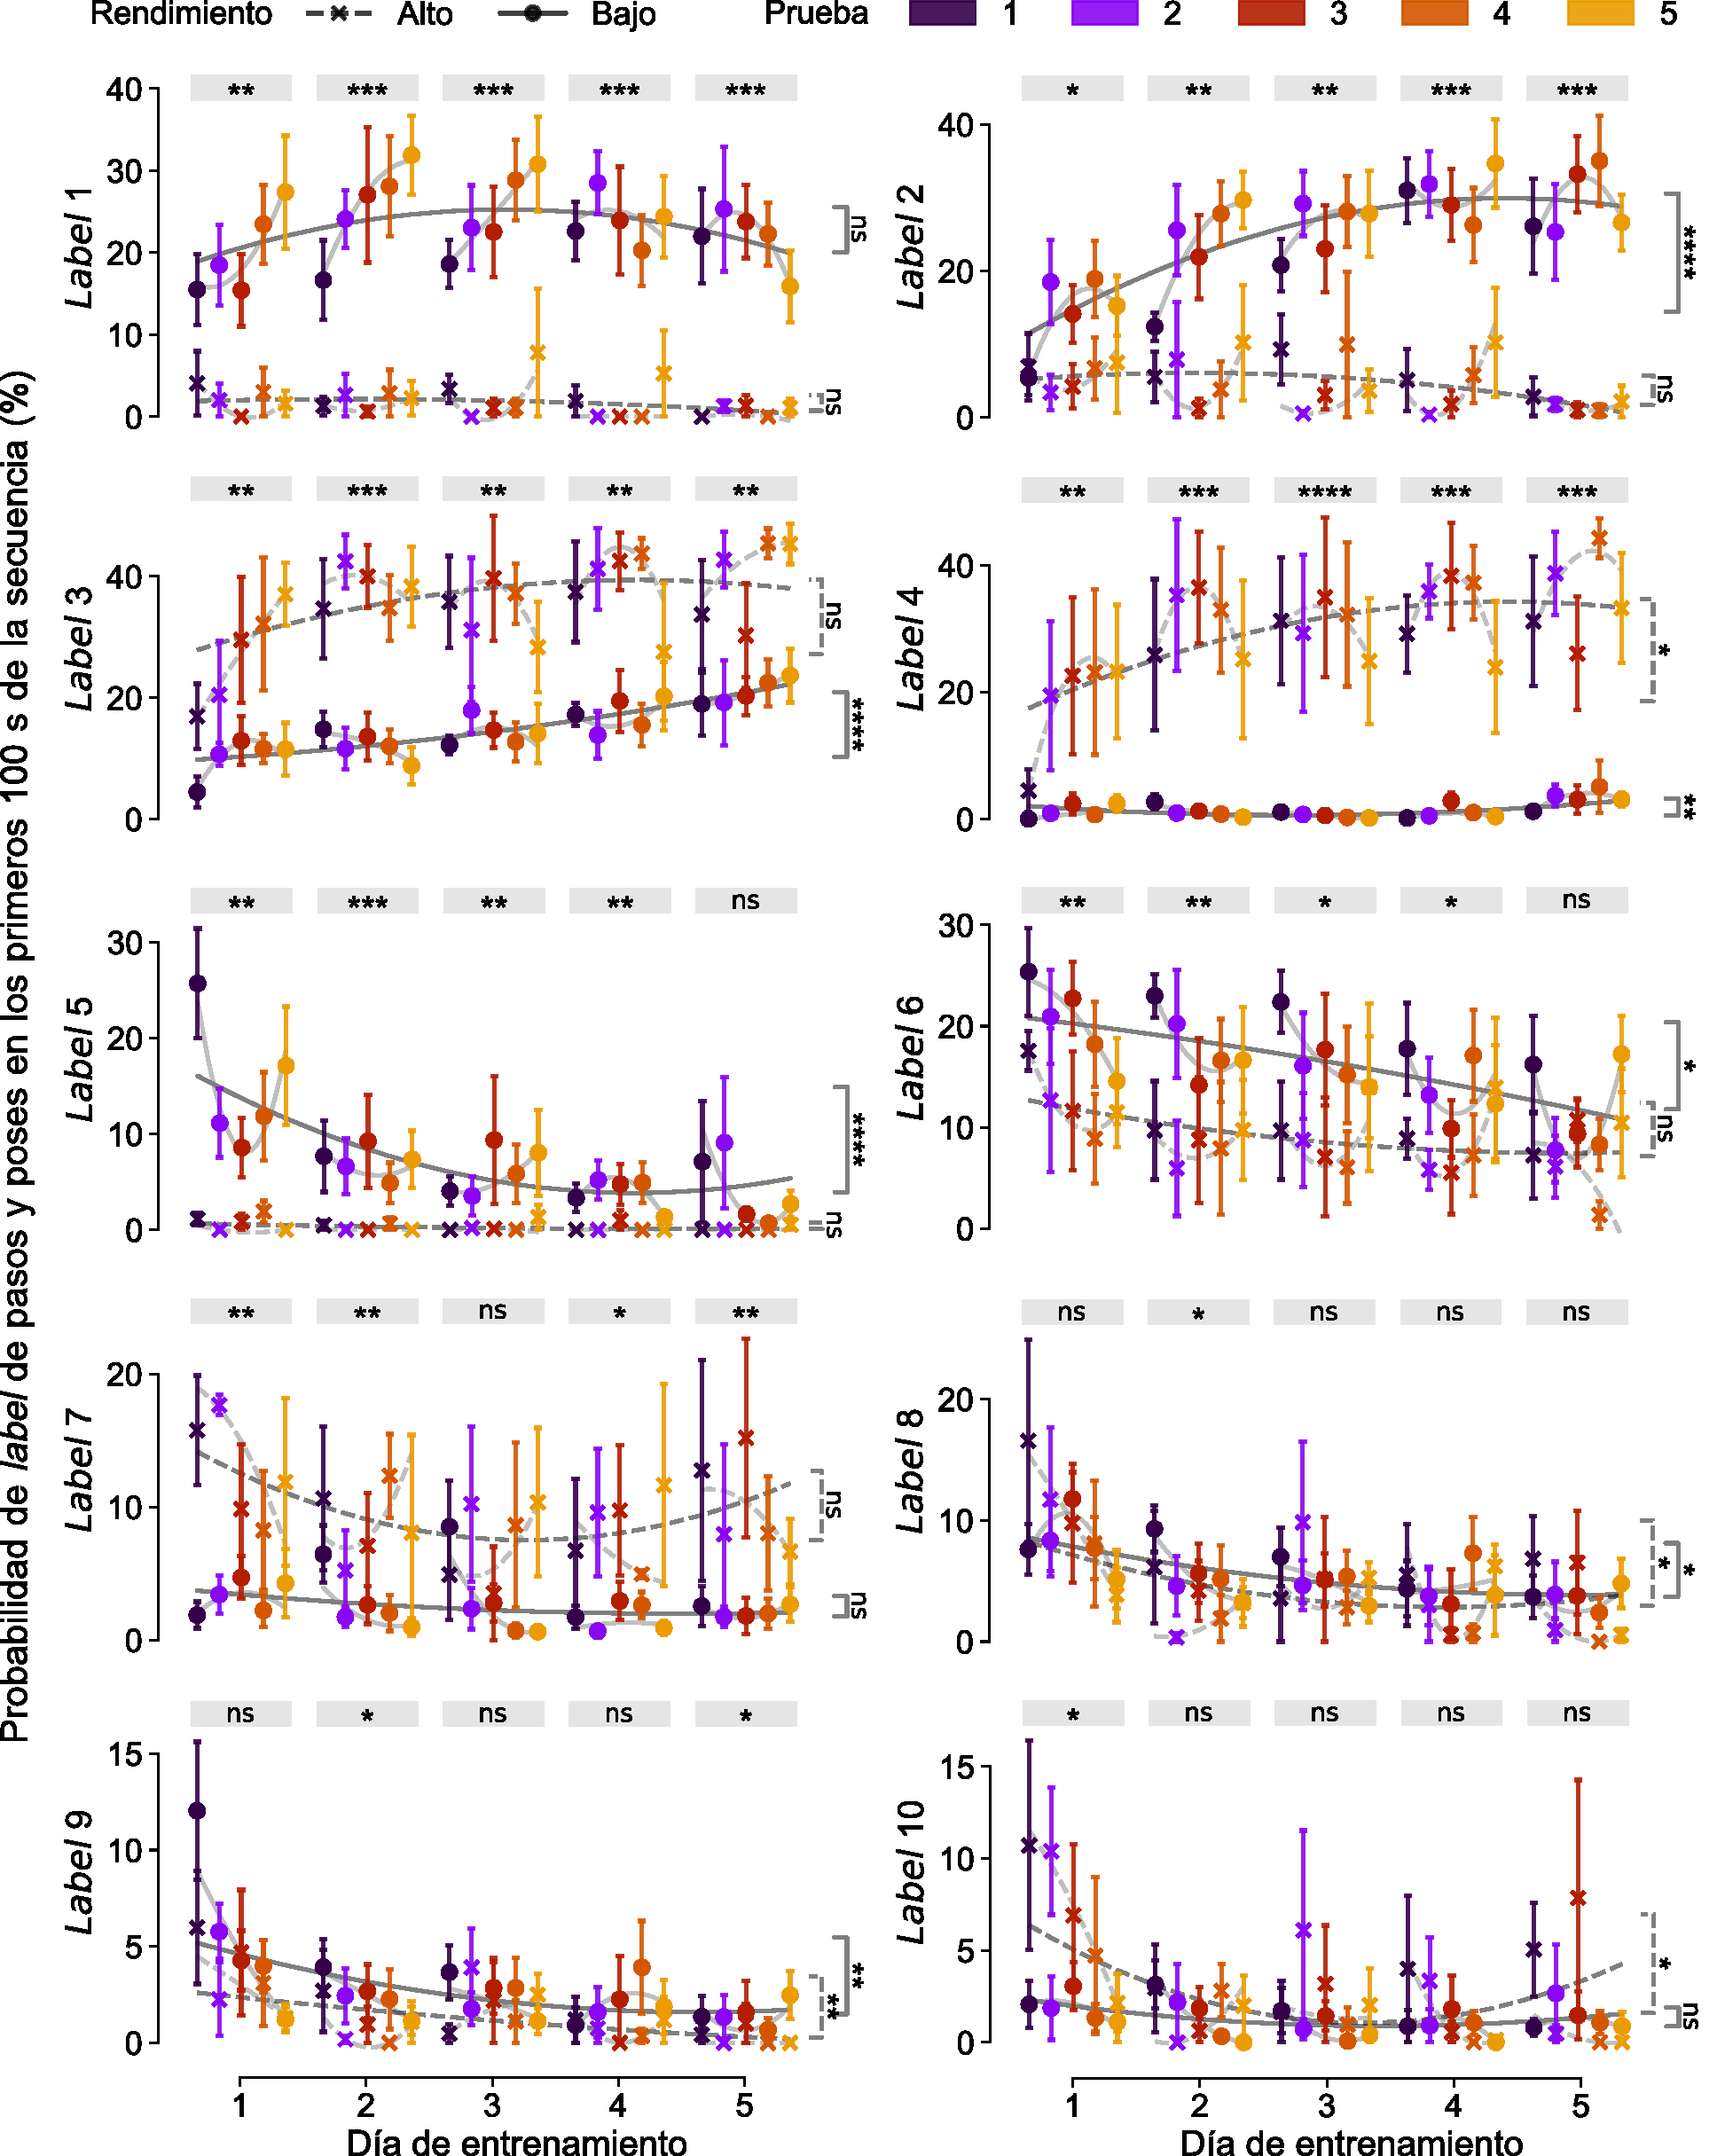
\includegraphics[width=0.99\linewidth]{figuras/capitulo4/probabilidades_labels_stp.pdf}
    \caption{\textbf{Cambios en las probabilidades de \textit{label} de pasos y poses en las secuencias de comportamiento.} Cada subfigura de la grilla representa la probabilidad de ocurrencia de un determinado \textit{label} durante los primeros 100 s de las pruebas rotarod, para cada día de entrenamiento y número de prueba realizada ese día. Los puntos muestran el promedio por grupo de rendimiento y las barras son el error estándar del promedio. Los rectángulos grises, en el margen superior de cada subfigura, indican los p-valores T-test entre grupos de rendimiento para cada día. Los corchetes en los márgenes derechos indican, para cada grupo de rendimiento, los p-valores \textit{one-way} ANOVA agrupando por día de entrenamiento.}
    \label{fig:capitulo4_probabilidades_labels_stp}
\end{figure}
\chapter*{Conclusiones}\label{cha:conclusiones}
\addcontentsline{toc}{chapter}{Conclusiones}
\markboth{Conclusiones}{Conclusiones}

\AddToShipoutPictureBG*{\put(0,0){%
        \parbox[b][\paperheight]{\paperwidth}{%
            \vfill
            \centering
            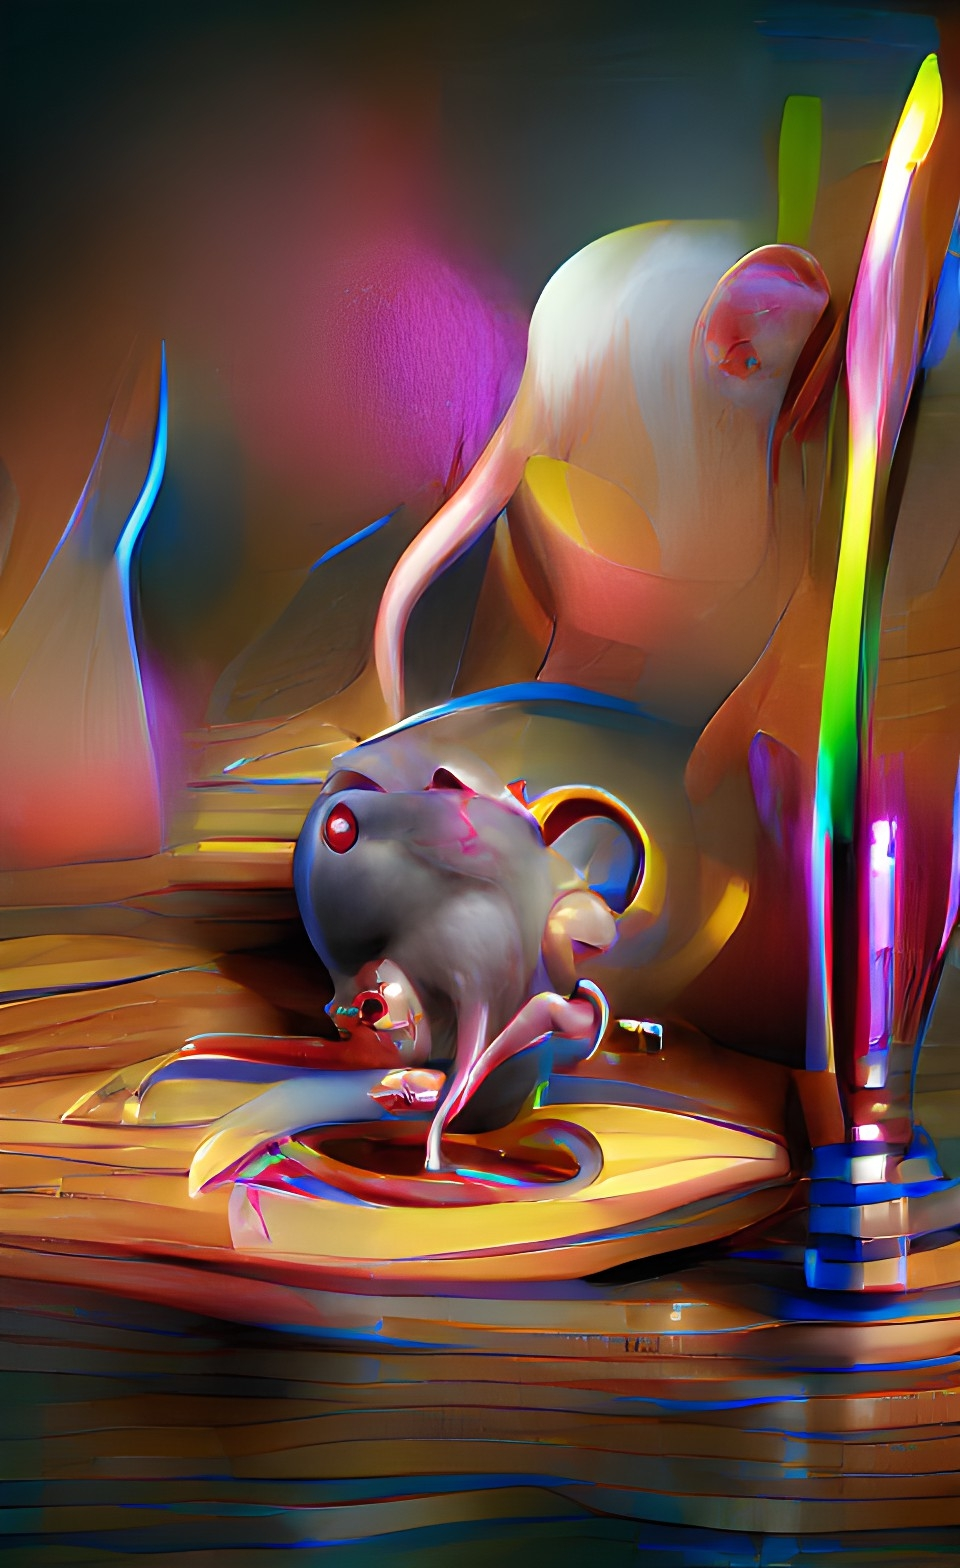
\includegraphics[width=\paperwidth,height=\paperheight,keepaspectratio]{%
                figuras/caratulas/conclusiones.jpg}\vfill
        }}}

\AddToShipoutPicture*{
    \begin{tikzpicture}[overlay, remember picture]
        \fill[white, opacity=0.75] (20, 24) rectangle (1, 22.5);
    \end{tikzpicture}}

\clearpage

Los avances tecnológicos recientes en aplicaciones del aprendizaje automático, redes neuronales artificiales profundas y técnicas de inferencia estadística son conducentes a un mejor entendimiento del comportamiento animal y de su relación con la actividad neuronal. En este trabajo hemos explorado diferentes maneras de representar el comportamiento de ratones durante su entrenamiento en la tarea rotarod con aceleración. Hemos corroborado que el algoritmo UMAP de reducción de la dimensión con segmentación \textit{watershed} es apto para la clasificación no supervisada de comportamiento animal durante la ejecución de esa tarea. A su vez, vimos que esta clasificación tiene prestaciones que son prometedoras para futuros estudios en combinación con registros de actividad neuronal. En particular, este método de análisis no supervisado permite automatizar el proceso de clasificación de comportamientos animales, brindando resultados potencialmente reproducibles entre evaluaciones y tiene la ventaja de cuantificar el comportamiento animal sin la necesidad de que intervenga manualmente un experto.

La tarea rotarod es usada tradicionalmente para evaluar impedimentos neurológicos en roedores (\autoref{cha:metodo_experimental}). Nosotros proponemos una visión renovada de esta tarea, bajo la luz de la neuroetología computacional, para analizar comportamientos descritos por múltiples características. Para que el campo de la neurociencia avance en el entendimiento de cómo el cerebro genera comportamientos ecológicamente relevantes en entornos naturales, debemos primero ser capaces de comprender las sutilezas del comportamiento animal complejo en situaciones lo más parecidas a las naturales. Esto significa estudiar el comportamiento animal sin restricciones físicas adicionales. Por desgracia, este sería un objetivo muy ambicioso de concretar. Afortunadamente, si bien la tarea rotarod presenta restricciones sobre la velocidad y el desplazamiento de los animales, constituye una excelente oportunidad para estudiar la adaptabilidad natural de sus secuencias comportamentales. En este sentido, consideramos a la tarea rotarod como una tarea natural de aprendizaje motor. Pues la manera en que los ratones adaptan su repertorio comportamental para resolver la tarea es completamente no trivial. A su vez, nuestros resultados indican que la variabilidad de estos repertorios comportamentales se reduce con el aprendizaje. También, observamos marcadas diferencias en los comportamientos de los ratones según su grado de aptitud física nato. Esta diferencia en aptitud física no se explica por su peso, sexo ni edad, aunque podría depender, por ejemplo, de su ritmo circadiano, si es que los animales son más activos en diferentes momentos del día, ya que las pruebas rotarod se realizaron por la mañana de forma regular.

El método más tradicional de representación del comportamiento, la métrica de latencia a caer, captura el progreso de los animales durante el entrenamiento y también las diferencias entre animales según su aptitud física. Adicionalmente, conseguimos definir otras métricas que describen de manera global cómo se desempeñan los ratones en la tarea, en múltiples aspectos (\autoref{cha:representacion_comportamiento}). De esta manera aportamos más información sobre el comportamiento de los ratones. Vimos que no solo aumenta la latencia a caer con el entrenamiento, sino que también aumentan la altura a la que los ratones dan pasos sobre el cilindro rotarod, mientras que la amplitud y la velocidad de los pasos se reduce. Además, registramos que las desviaciones en las ejecuciones comportamentales de los ratones se reduce con el entrenamiento. Y observamos que la mayoría de los cambios más significativos en estas métricas se dan en la segunda prueba del primer día de entrenamiento, mostrando la rapidez con la que los ratones se adaptan a nuevas situaciones. El aprendizaje motor se divide en dos fases: una fase temprana donde hay una mejora abrupta en la ejecución de la tarea, y una fase tardía donde el rendimiento mejora de manera asintótica. Curiosamente, en ambas fases participan diferentes estructuras cerebrales. Sin embargo, la latencia al caer no captura correctamente la fase tardía del aprendizaje de la tarea de rotarod. Por eso este tipo de estudios de comportamiento multidimensional permite entender las peculiaridades del aprendizaje con mayor detalle \cite{luft_motor_learning}.

Por último, hemos mostrado el potencial de esta clasificación no supervisada de poses para estudiar detalladamente la estructura temporal del comportamiento animal. En las secuencias de comportamientos, se observan marcadas preferencias por iniciar y terminar las pruebas rotarod usando determinadas categorías de comportamientos (\textit{labels}). En el \autoref{cha:mapas_comportamiento} obtuvimos dos conjuntos de \textit{labels}: uno a partir de los espectros \textit{wavelet} de partes del cuerpo de los ratones y otro a partir de características de pasos y poses adoptadas por los ratones. Observamos que los \textit{labels} de pasos y poses separan más fuertemente a los ratones según su grupo de rendimiento, comparados con los \textit{labels} \textit{wavelet}. En ambos casos, se observa que la variabilidad en las probabilidades de labels en las secuencias de comportamiento se reduce con el entrenamiento. A su vez, la entropía de las proyecciones UMAP también se reduce con los días de entrenamiento, sosteniendo que la variabilidad en las estrategias de comportamiento usadas por los ratones se reduce con el aprendizaje. El uso de mapas UMAP de dimensión reducida permite un enfoque holístico en el estudio del comportamiento: permite estudiar los efectos y cambios de múltiples características comportamentales en una conveniente representación de fácil visualización.

Esperamos que estos métodos de clasificación no supervisada de comportamiento, con algoritmos de reducción de dimensión como las proyecciones UMAP con segmentación \textit{watershed}, permitan evaluar detalladamente el desempeño físico durante la ejecución de otros tipos de tareas motoras y que también permitan cuantificar cambios a raíz de impedimentos motores como consecuencia de enfermedades neurodegenerativas. Existe evidencia experimental mostrando una reducción en la latencia a caer en modelos de la enfermedad de Parkinson y de esclerosis lateral amiotrófica \cite{costa_motor_learning, campos_parkinson}; sin embargo, estos trabajos utilizan solo la latencia a caer como métrica de rendimiento de los animales. Nosotros postulamos que el estudio detallado de los patrones de comportamiento durante la ejecución de tareas nos permitirá la detección temprana de impedimentos motores y la comparación de diferencias entre modelos experimentales de enfermedades neurodegenerativas que ayude a avanzar en la compresión de los circuitos neuronales subyacentes \cite{alfieri_motor_deficit}.

Como sucesión del trabajo desarrollado en la tesis de licenciatura, alcanzamos y superamos los objetivos propuestos hace un año y conseguimos resultados novedosos. Habíamos propuesto incorporar el uso de espectros \textit{wavelet} para capturar la dinámica del movimiento de las partes del cuerpo de los ratones. No solo hicimos eso, sino que también agregamos un segundo conjunto de características comportamentales al análisis: las características de pasos y poses. Otro de los objetivos propuestos fue estudiar el comportamiento animal durante el aprendizaje de una tarea motora. Y esto también fue alcanzado. Adicionalmente, parte del código implementado para el preprocesamiento y análisis del comportamiento animal, utilizado a lo largo de este trabajo, puede consultarse en nuestros repositorios \href{https://github.com/alvaro-concha/animal-behavior-preprocessing}{\color{blue}{animal-behavior-preprocessing}} y \href{https://github.com/alvaro-concha/animal-behavior-analysis}{\color{blue}{animal-behavior-analysis}}.

\cleardoublepage
\phantomsection
\addcontentsline{toc}{chapter}{Referencias}
\printbibliography[title=Referencias]
{
  \vspace*{\fill}
  Las carátulas de este trabajo fueron generadas artificialmente usando \href{https://www.wombo.art/}{WOMBO Dream}.
}

\begin{appendix}
    \chapter{Análisis de características}\label{cha:apendice_caracteristicas}

    Figuras suplementarias relacionadas con el análisis de las características comportamentales extraídas.

    \section{Captura de movimiento}\label{sec:apendice_captura_movimiento}

    \begin{figure}[htbp]
        \centering
        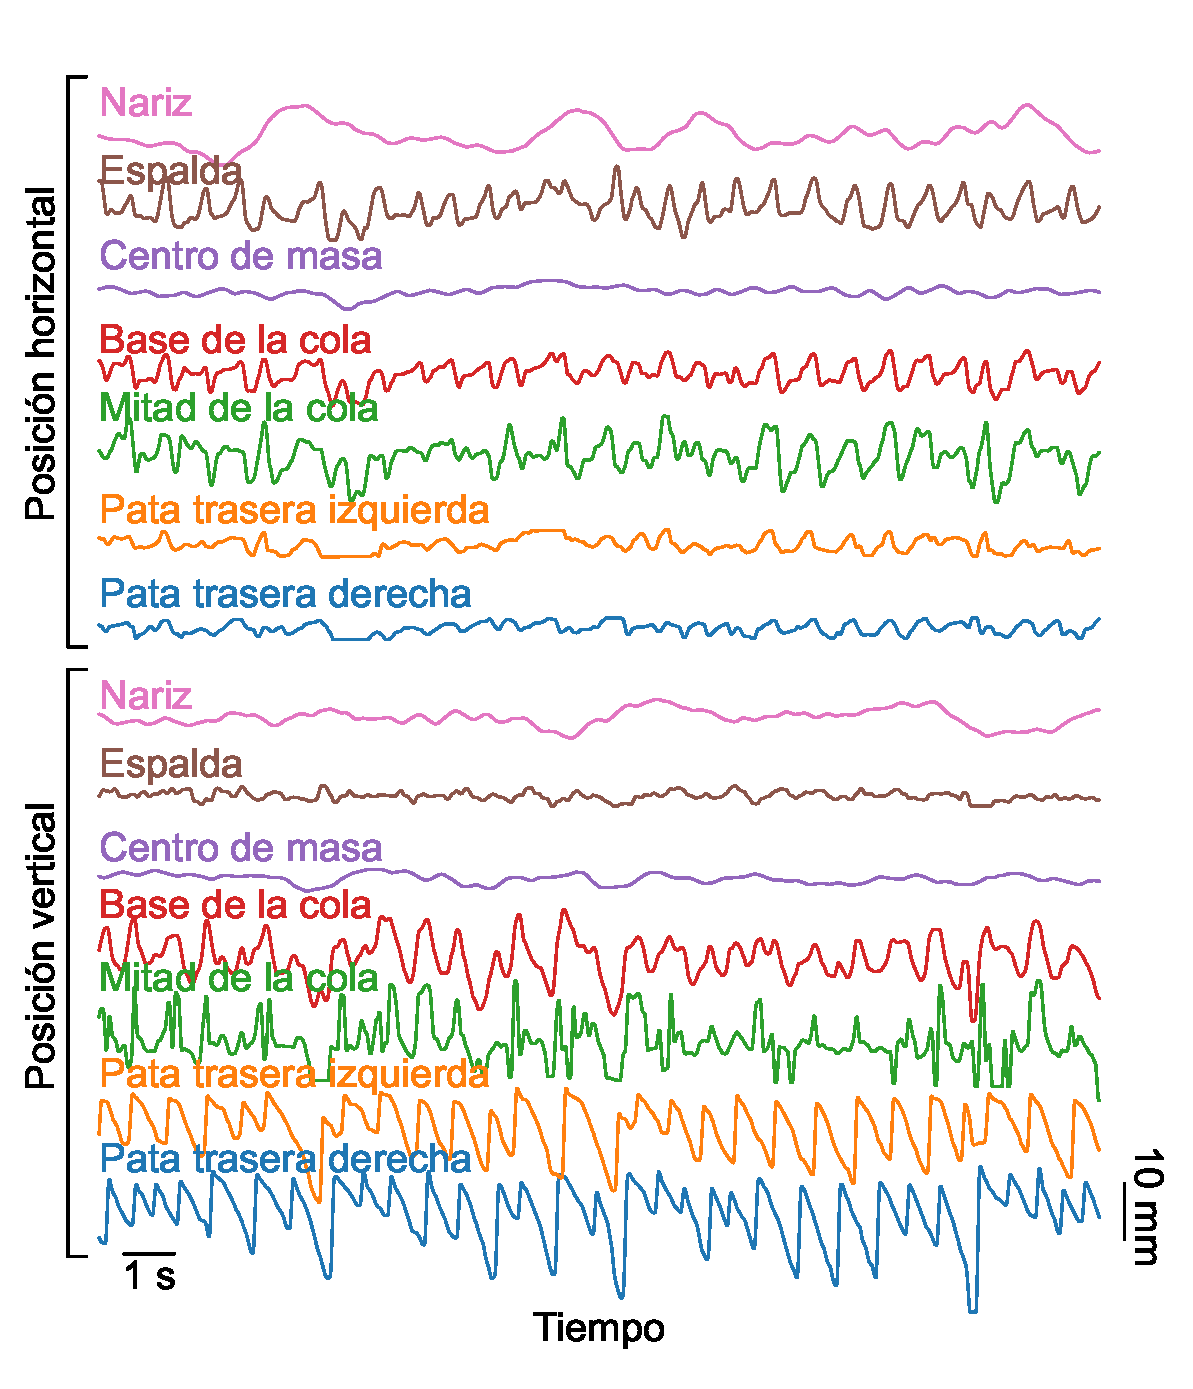
\includegraphics[width=0.6\linewidth]{figuras/capitulo2/posiciones.pdf}
        \caption{\textbf{Posiciones de los marcadores en el tiempo.}
            Seguimiento de marcadores digitales, entre los 75 y 95 s de iniciada una prueba rotarod.
            Se muestran las posiciones horizontales y verticales de los diferentes marcadores en el tiempo.}
        \label{fig:capitulo2_posiciones}
    \end{figure}

    \clearpage

    \section{Ángulos entre partes del cuerpo}\label{sec:apendice_angulos_entre_partes}

    \begin{figure}[htbp]
        \centering
        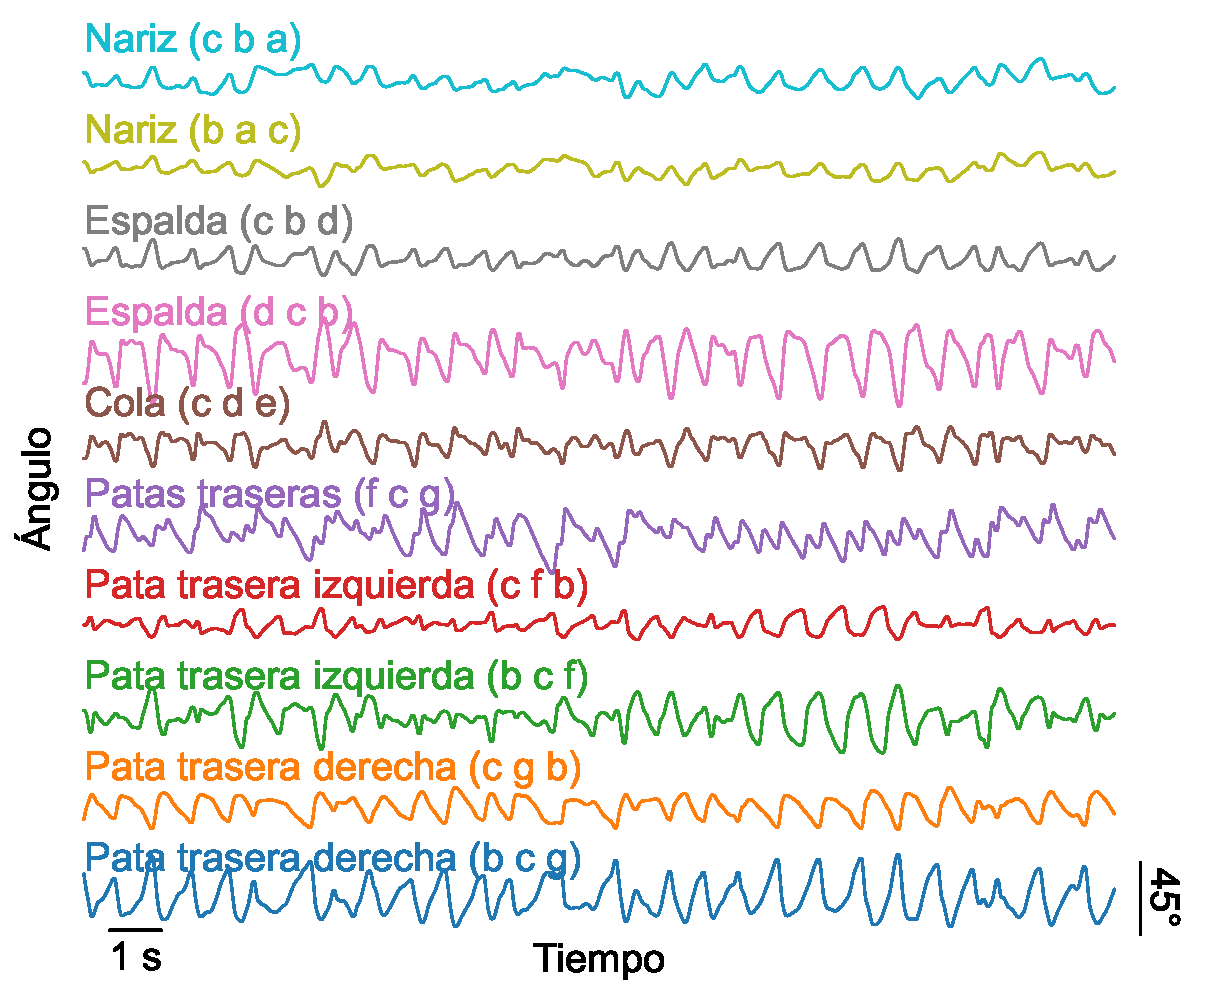
\includegraphics[width=0.6\linewidth]{figuras/capitulo2/angulos.pdf}
        \caption{\textbf{Ángulos de partes del cuerpo en el tiempo.}
            Valores de los ángulos entre los 75 y 95 s de iniciada una prueba rotarod (ídem \autoref{fig:capitulo2_posiciones}).
            Cada ángulo está definido por un triplete (i j k) con i, j, k símbolos de los marcadores.
            Marcadores: (a) nariz, (b) espalda, (c) centro de masa, (d) base de la cola, (e) mitad de la cola, (f) pata trasera izquierda, (g) pata trasera derecha.}
        \label{fig:capitulo2_angulos}
    \end{figure}

    \clearpage

    \section{Espectros \textit{wavelet} y PCA}\label{sec:apendice_pca_wavelet}

    \begin{figure}[htbp]
        \centering
        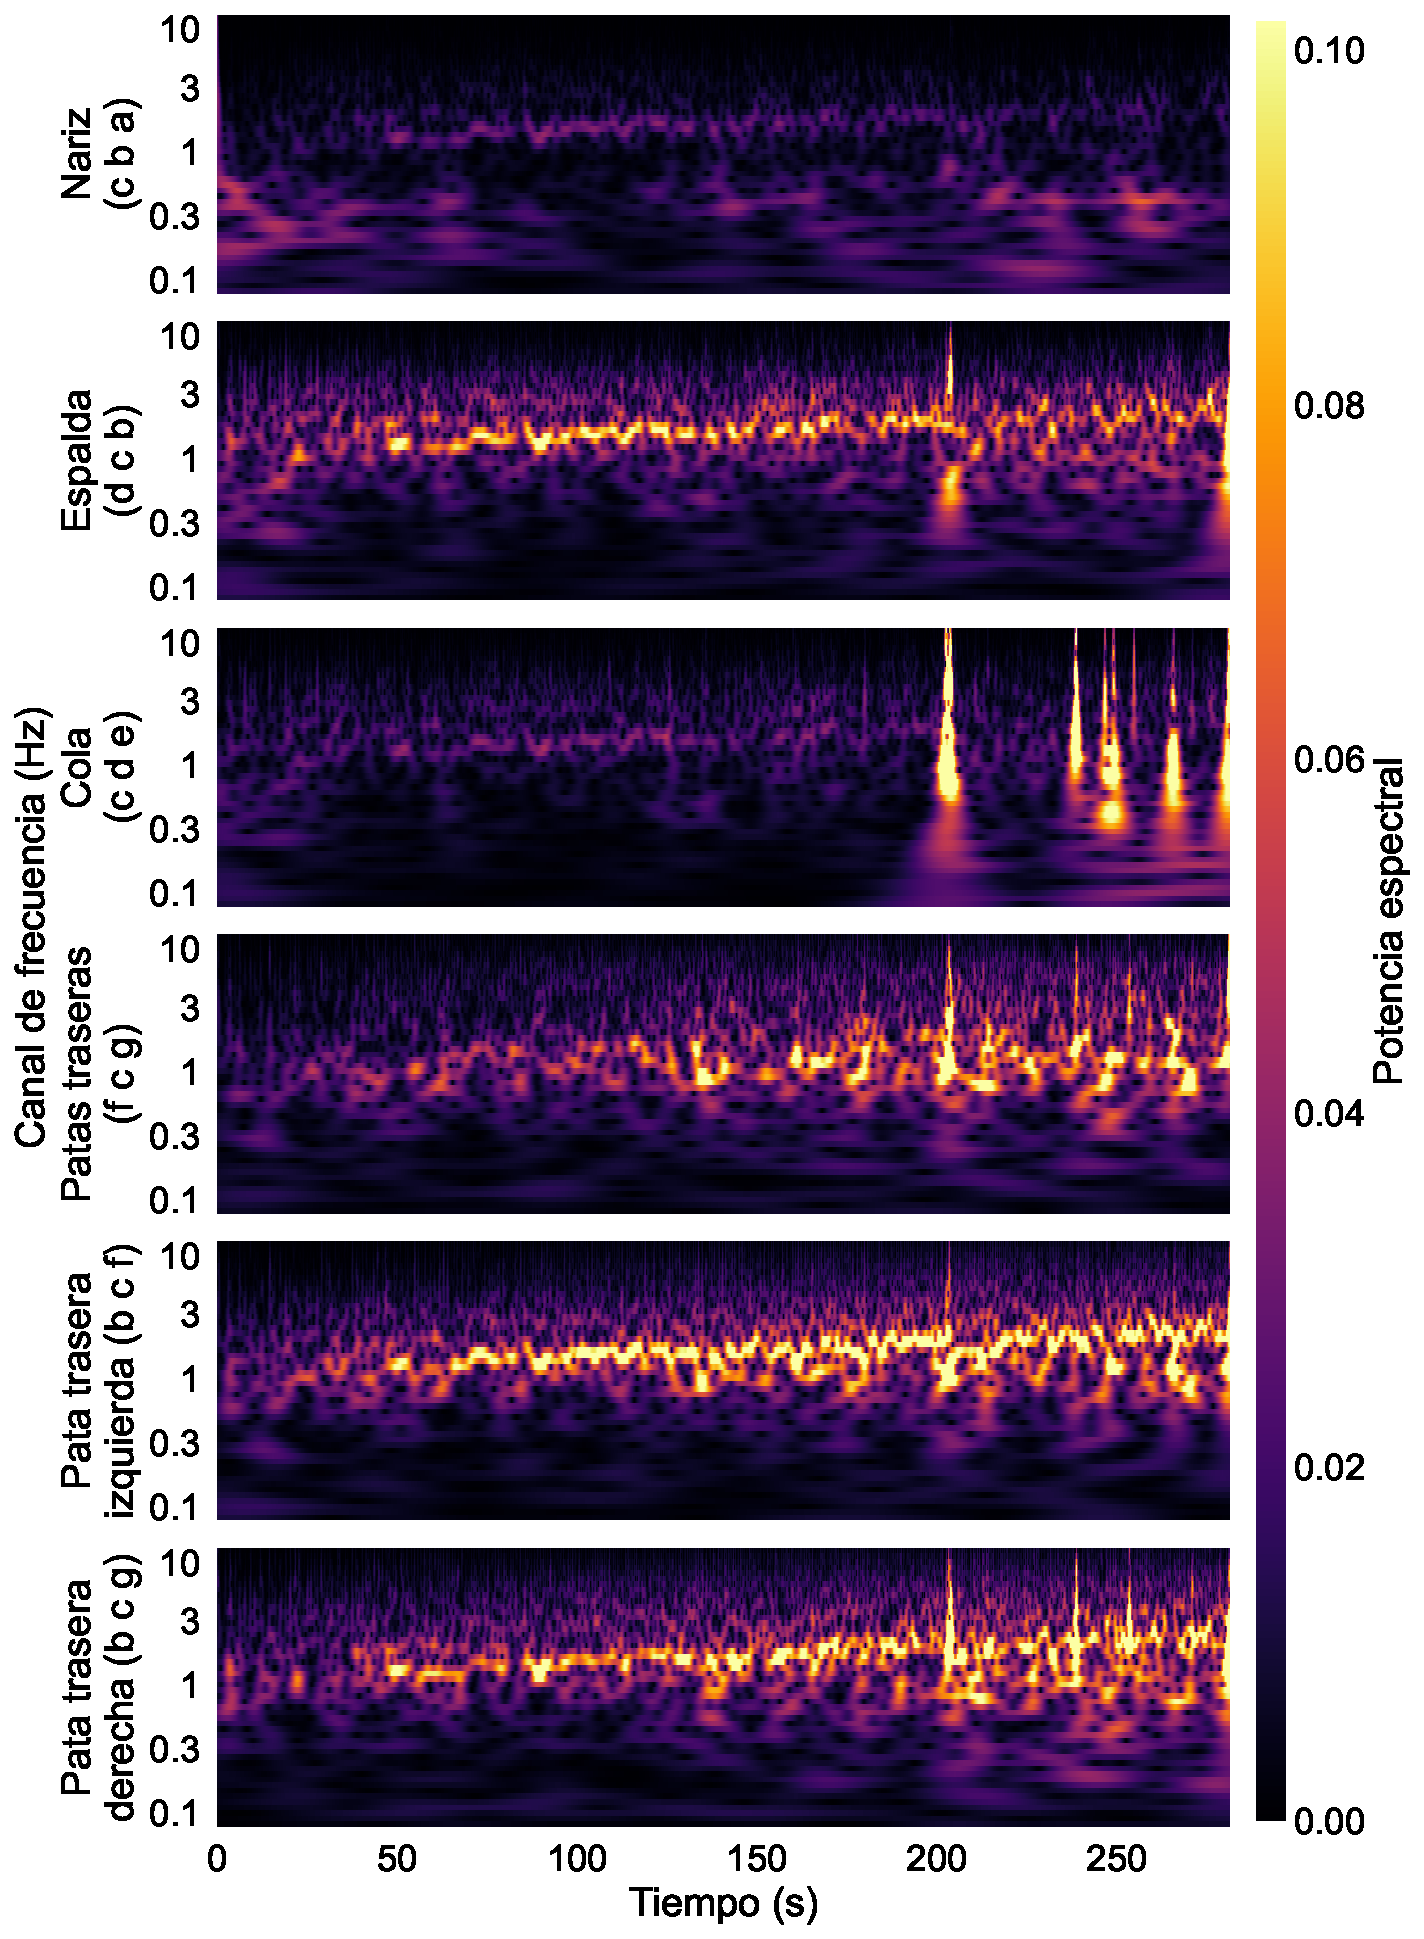
\includegraphics[width=0.7\linewidth]{figuras/capitulo2/espectros_wavelet.pdf}
        \caption{\textbf{Espectros \textit{wavelet} en el tiempo.}
            Espectros de algunos ángulos entre marcadores durante una prueba rotarod (ídem \autoref{fig:capitulo2_posiciones}).
            Cada ángulo está definido por un triplete (i j k) con i, j, k símbolos de los marcadores.
            Marcadores: (a) nariz, (b) espalda, (c) centro de masa, (d) base de la cola, (e) mitad de la cola, (f) pata trasera izquierda, (g) pata trasera derecha.}
        \label{fig:capitulo2_espectros_wavelet}
    \end{figure}

    \begin{figure}[htbp]
        \centering
        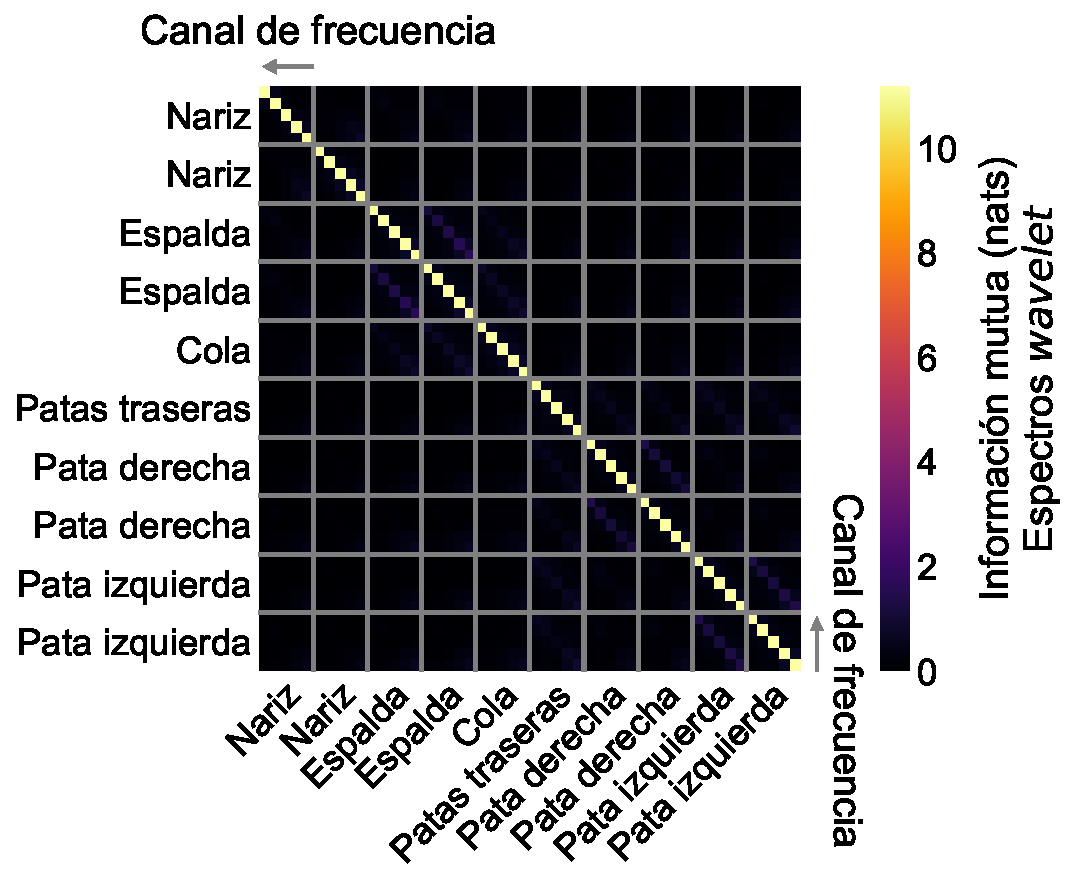
\includegraphics[width=0.7\linewidth]{figuras/capitulo4/mi_mean_wav.pdf}
        \caption{\textbf{Grupos de partes del cuerpo que dependen muy levemente entre sí según sus espectros \textit{wavelet}.}
            Información mutua entre los diferentes canales de frecuencia de los espectros \textit{wavelet} de los ángulos.
            Se observan grupos de ángulos que dependen muy levemente entre sí: patas traseras, espalda-cola y nariz.}
        \label{fig:capitulo2_mi_mean_wav}
    \end{figure}

    \begin{figure}[htbp]
        \centering
        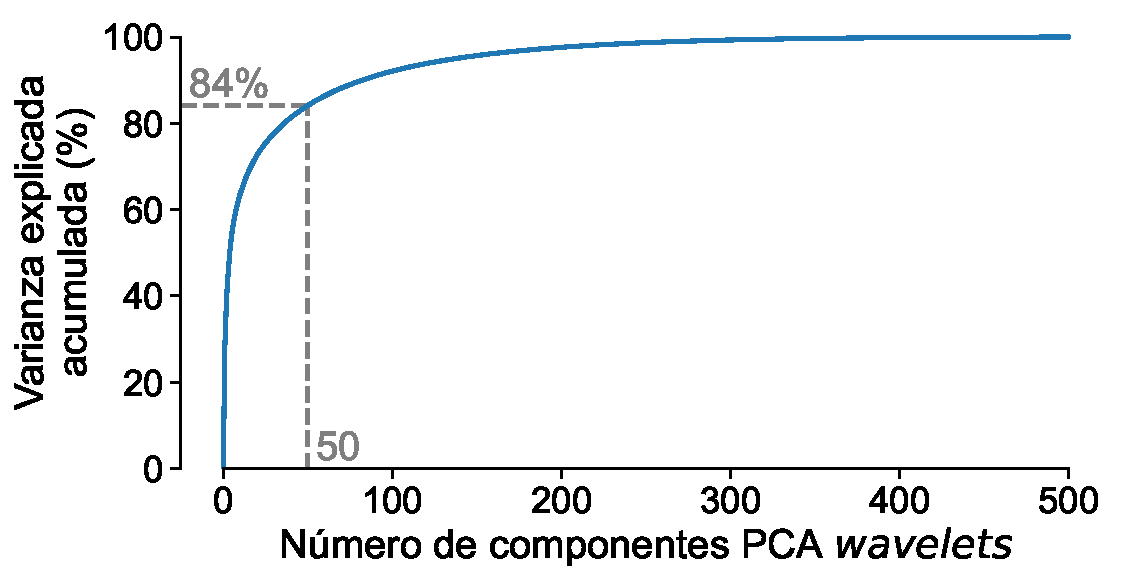
\includegraphics[width=0.7\linewidth]{figuras/capitulo4/varianza_pca.pdf}
        \caption{\textbf{Las 50 primeras componentes principales explican el 84\% de la varianza de los espectros \textit{wavelet}.}
            Varianza explicada acumulada según el número de componentes PCA de los espectros \textit{wavelet}.}
        \label{fig:capitulo4_varianza_pca}
    \end{figure}

    \begin{figure}[htbp]
        \centering
        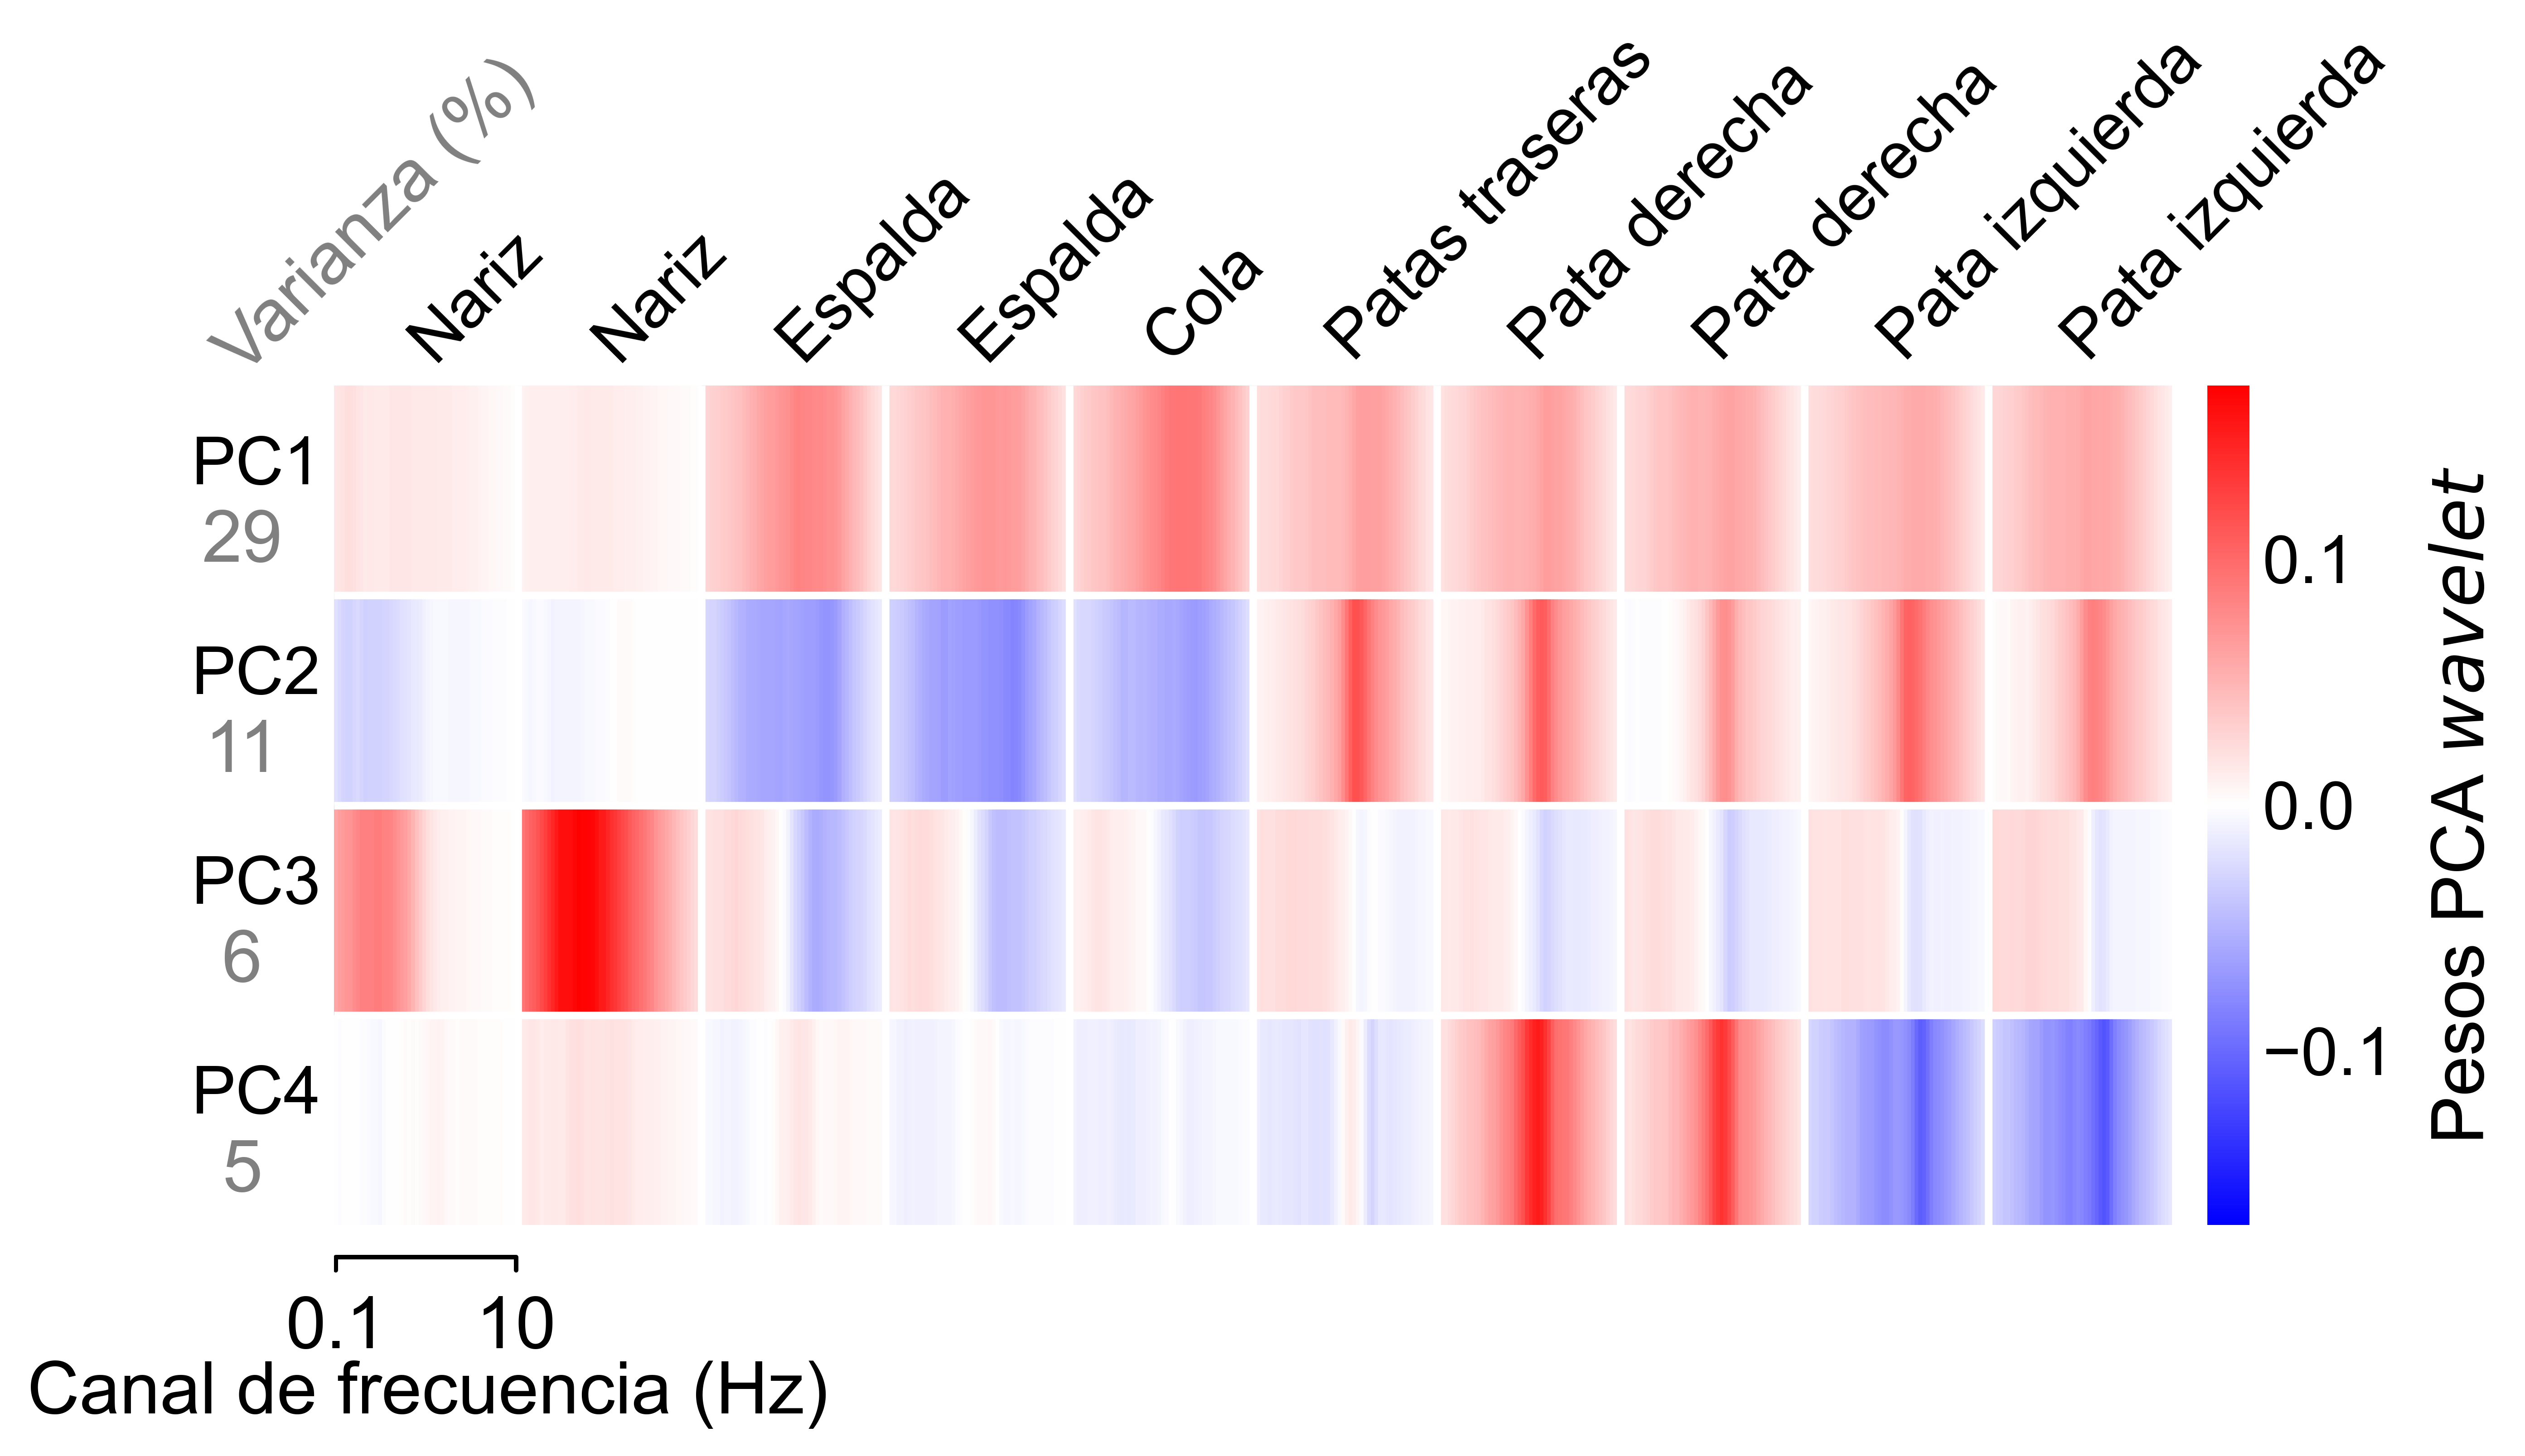
\includegraphics[width=0.8\linewidth]{figuras/capitulo4/pesos_pca.png}
        \caption{\textbf{La primera componente principal de los espectros \textit{wavelet} sigue a la frecuencia espectral promedio.}
            Pesos de las 4 primeras componentes PCA de los espectros \textit{wavelet}, según los canales de frecuencia y las partes del cuerpo involucradas.}
        \label{fig:capitulo4_pesos_pca}
    \end{figure}

    \begin{figure}[htbp]
        \centering
        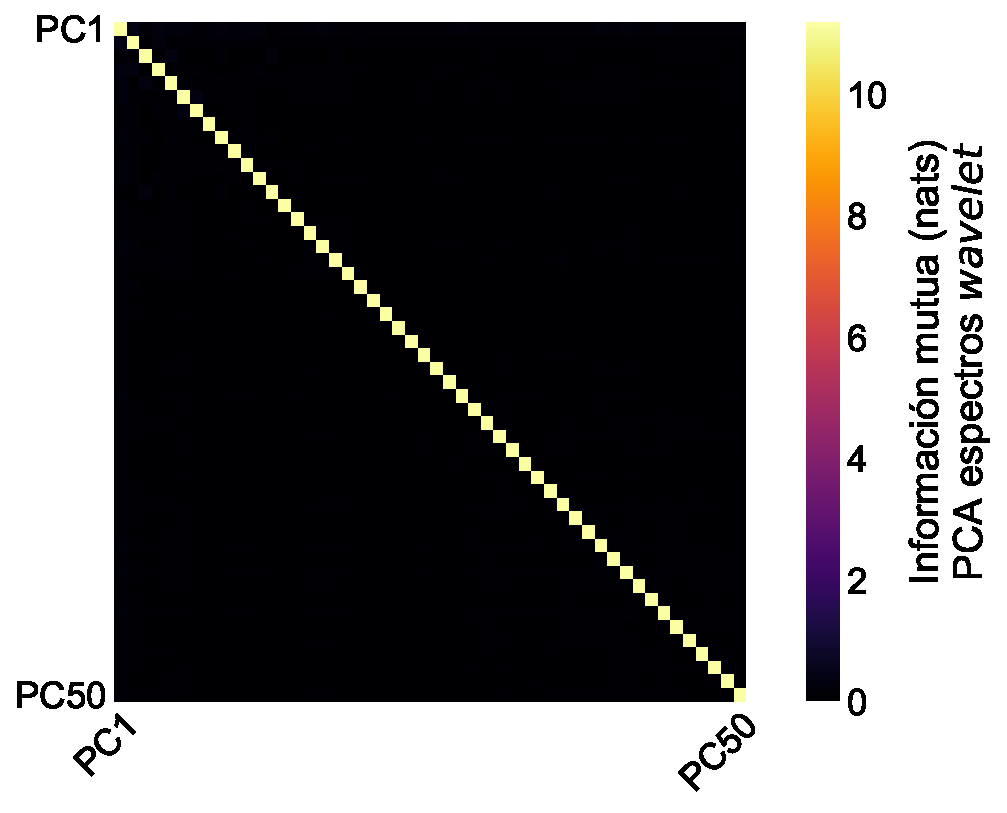
\includegraphics[width=0.7\linewidth]{figuras/capitulo4/mi_pca_wav.pdf}
        \caption{\textbf{Componentes PCA de los espectros \textit{wavelet} son independientes entre sí.}
            Información mutua entre las primeras 50 componentes principales de los espectros \textit{wavelet} de los ángulos.}
        \label{fig:capitulo4_mi_pca_wav}
    \end{figure}

    \begin{figure}[htbp]
        \centering
        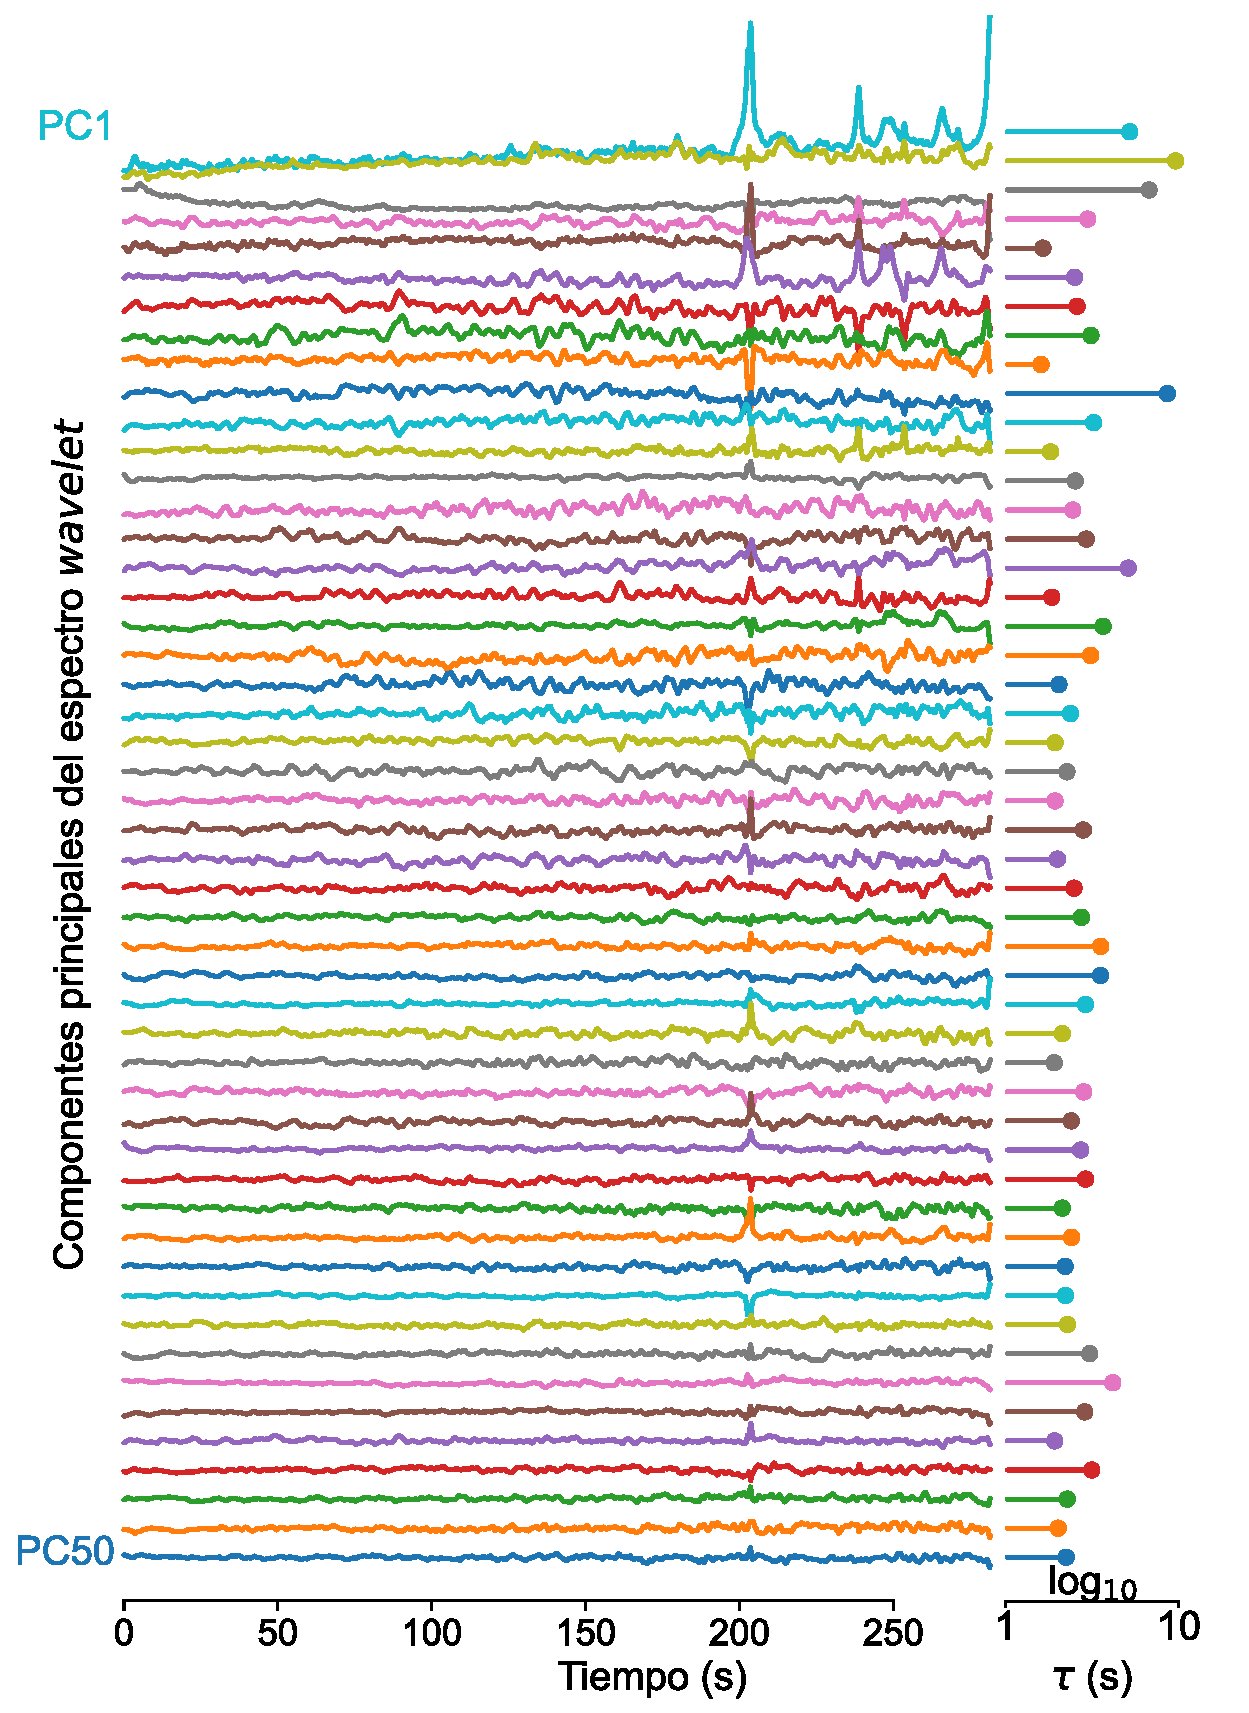
\includegraphics[width=0.7\linewidth]{figuras/capitulo4/componentes_pca.pdf}
        \caption{\textbf{Primeras 50 componentes PCA de los espectros \textit{wavelet}.}
            Ejemplo de los valores que adoptan las primeras 50 componentes PCA de los espectros \textit{wavelet} en una prueba rotarod (ídem \autoref{fig:capitulo2_posiciones}).
            En el margen izquierdo se muestra el tiempo de autocorrelación $\tau$ de cada componente en la prueba.}
        \label{fig:capitulo4_componentes_pca}
    \end{figure}

    \clearpage

    \section{Características de pasos y poses}\label{sec:apendice_pasos_poses}

    \begin{figure}[htbp]
        \centering
        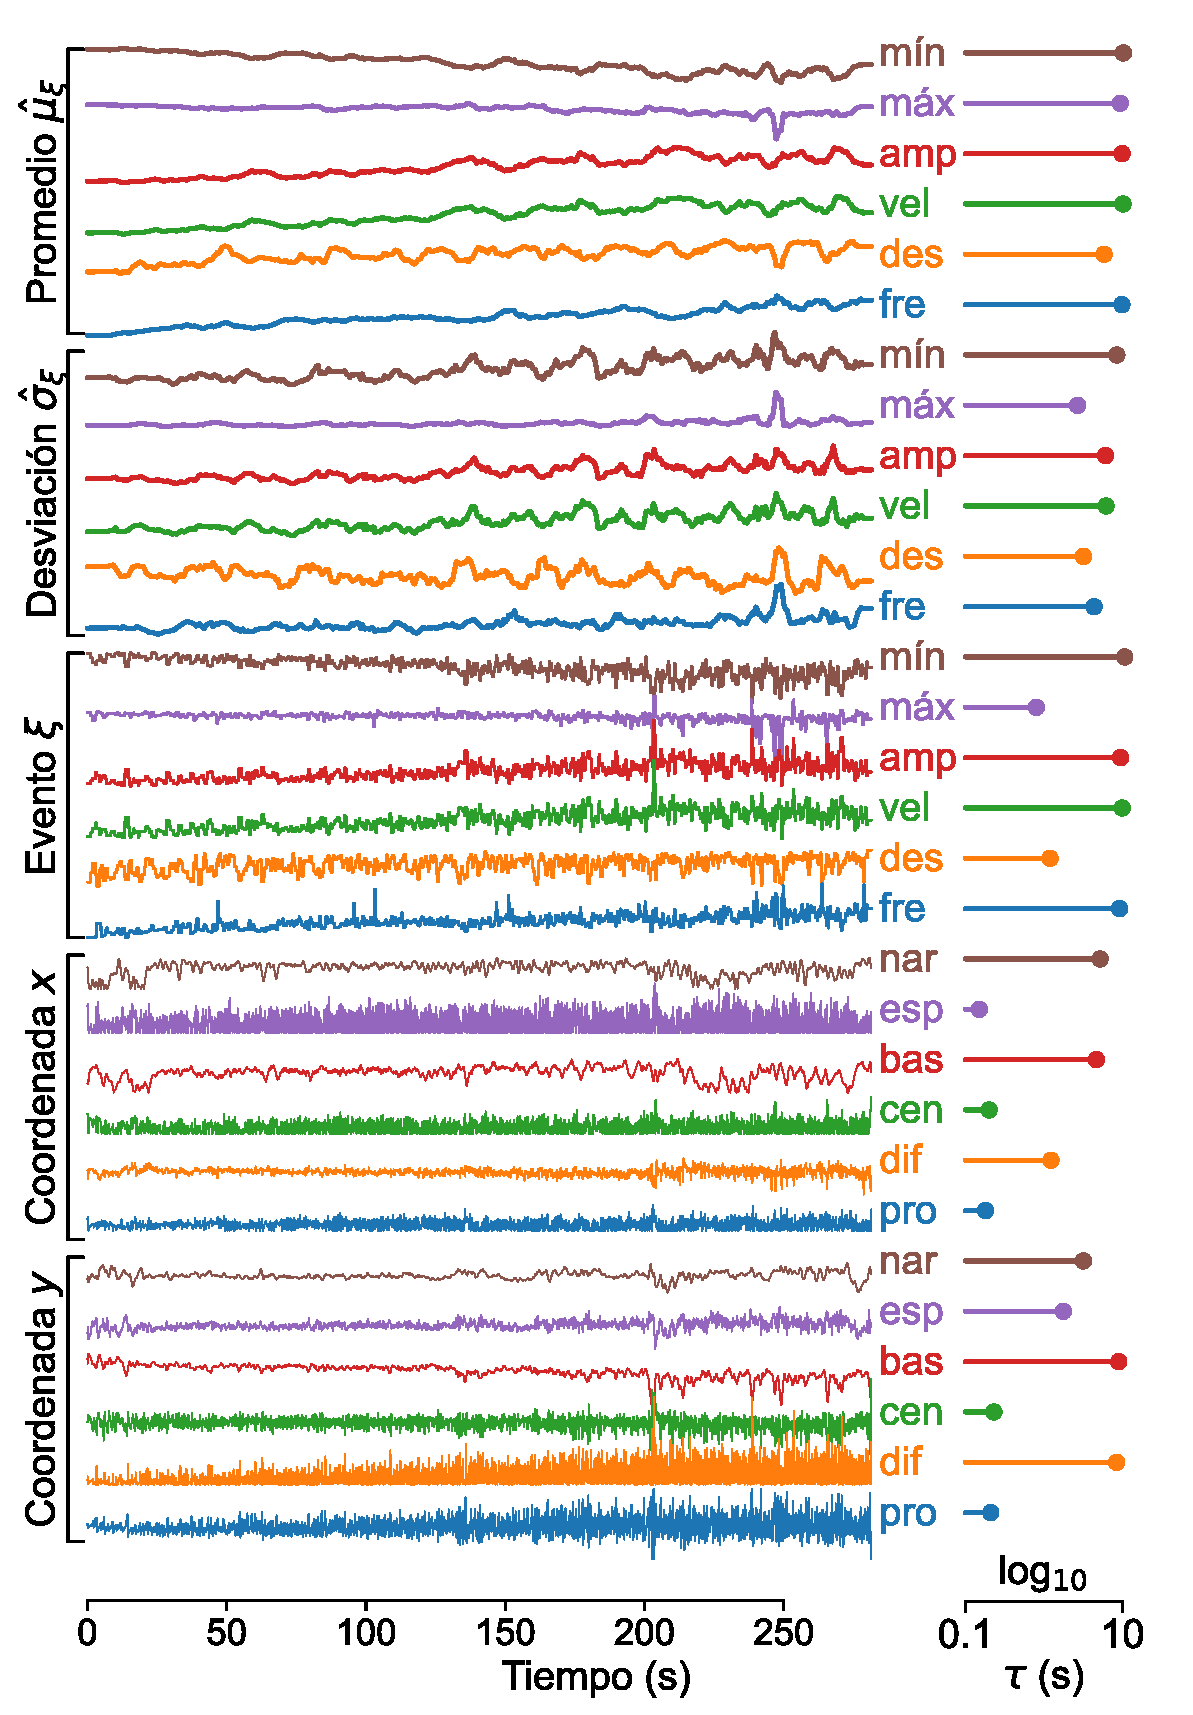
\includegraphics[width=0.7\linewidth]{figuras/capitulo4/caracteristicas_pasos_poses.pdf}
        \caption{\textbf{Características de pasos y poses.}
            Ejemplo de los valores que adoptan las características de pasos y poses en una prueba rotarod (ídem \autoref{fig:capitulo2_posiciones}).
            En el margen izquierdo se muestra el tiempo de autocorrelación $\tau$ de cada característica en la prueba.
            Abreviaturas: (min) altura mínima, (max) altura máxima, (amp) amplitud, (vel) velocidad, (des) desfasaje, (fre) frecuencia,
            (nar) nariz, (esp) espalda, (bas) base de la cola, (cen) centro de masa, (dif) diferencia entre patas traseras, (pro) promedio entre patas traseras.}
        \label{fig:capitulo4_caracteristicas_pasos_poses}
    \end{figure}

    \begin{figure}[htbp]
        \centering
        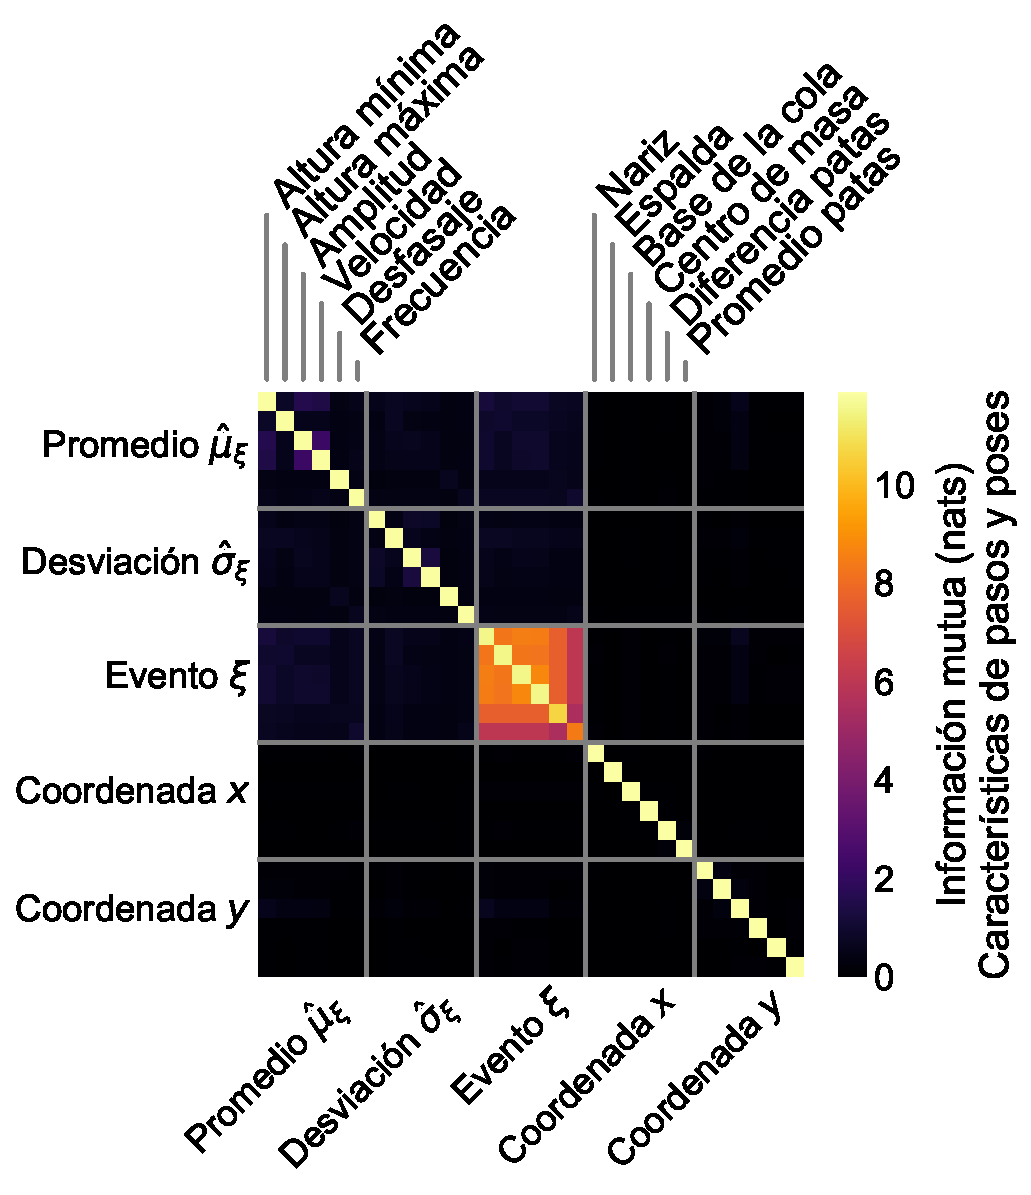
\includegraphics[width=0.7\linewidth]{figuras/capitulo4/mi_scaler_stp.pdf}
        \caption{\textbf{Características de pasos dependen más fuertemente entre sí en los eventos.}
            Información mutua entre las diferentes las diferentes variables de las características de los pasos y poses.}
        \label{fig:capitulo4_mi_scaler_stp}
    \end{figure}

    \begin{figure}[htbp]
        \centering
        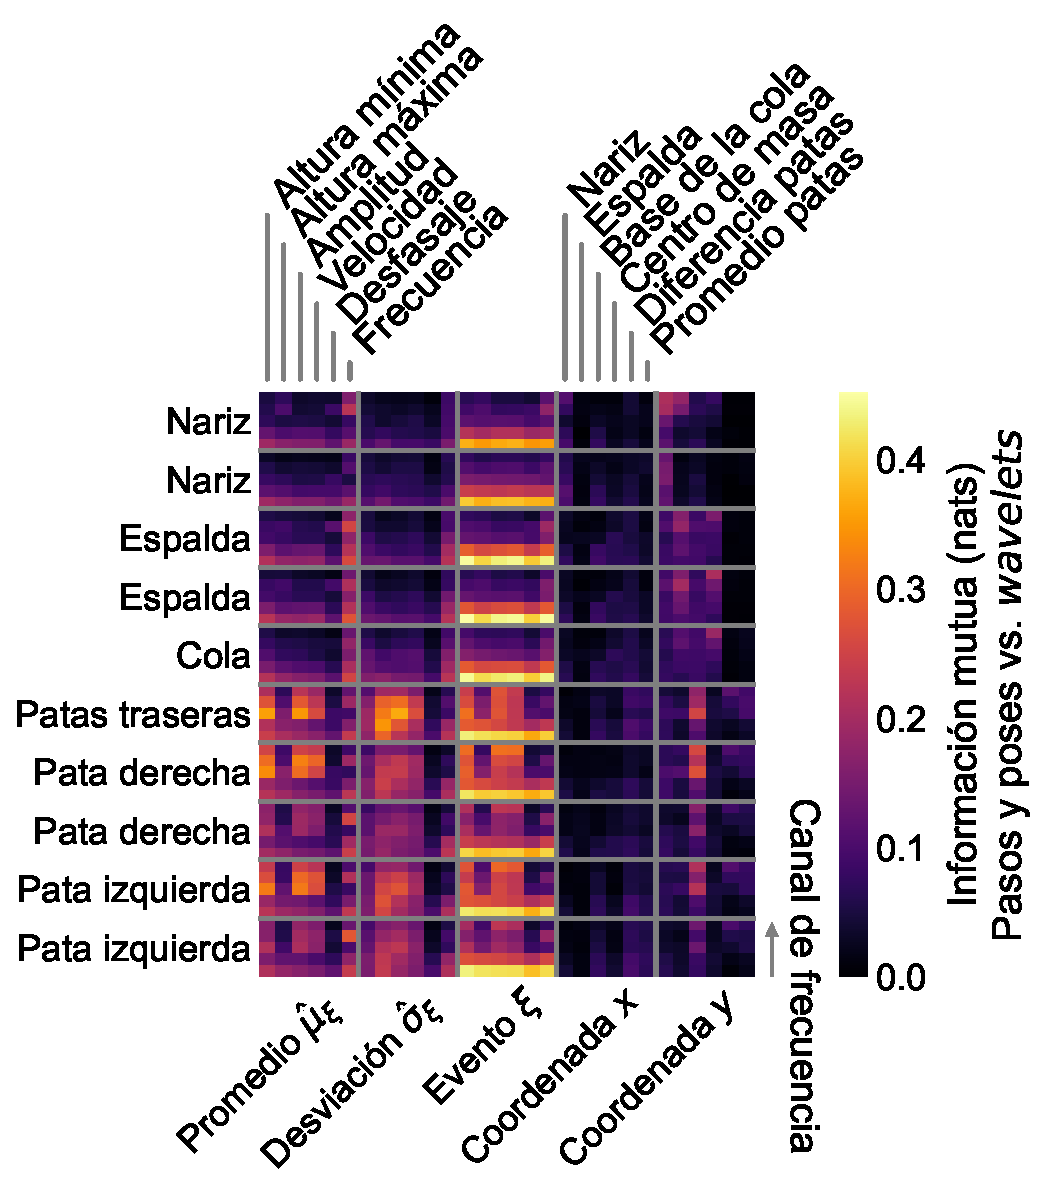
\includegraphics[width=0.75\linewidth]{figuras/capitulo4/mi_mean_wav_scaler_stp.pdf}
        \caption{\textbf{Información mutua pasos y poses vs. espectros \textit{wavelet}.}}
        \label{fig:capitulo4_mi_mean_wav_scaler_stp}
    \end{figure}

    \begin{figure}[htbp]
        \centering
        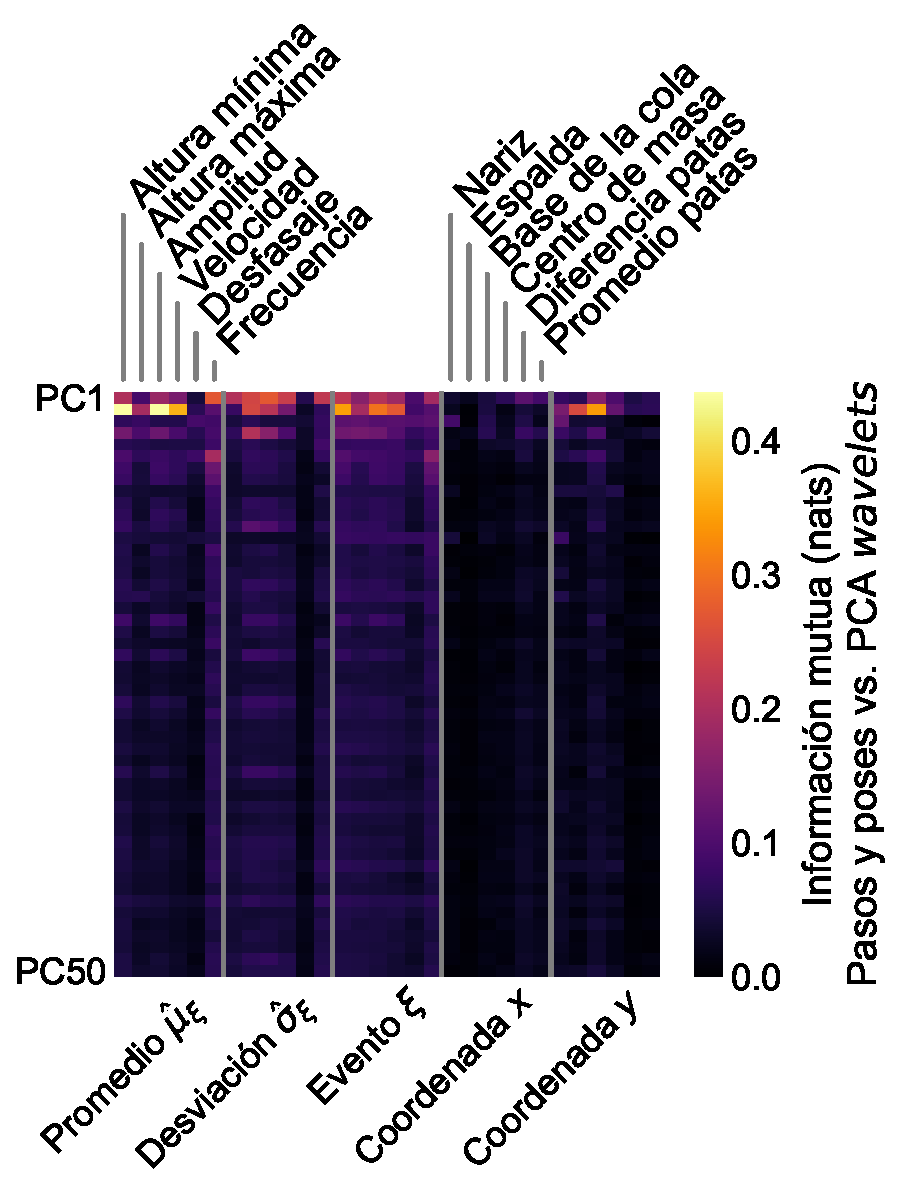
\includegraphics[width=0.7\linewidth]{figuras/capitulo4/mi_pca_wav_scaler_stp.pdf}
        \caption{\textbf{Información mutua pasos y poses vs. PCA \textit{wavelets}.}}
        \label{fig:capitulo4_mi_pca_wav_scaler_stp}
    \end{figure}

    \clearpage

    \chapter{Métricas de comportamiento}\label{cha:apendice_metricas}

    Figuras suplementarias acerca de la evolución de las diferentes métricas comportamentales calculadas a partir de las características de pasos durante los primeros 100 s de la ejecución de las pruebas rotarod.

    \clearpage

    \section{Promedio}\label{sec:apendice_promedio}

    \begin{figure}[htbp]
        \centering
        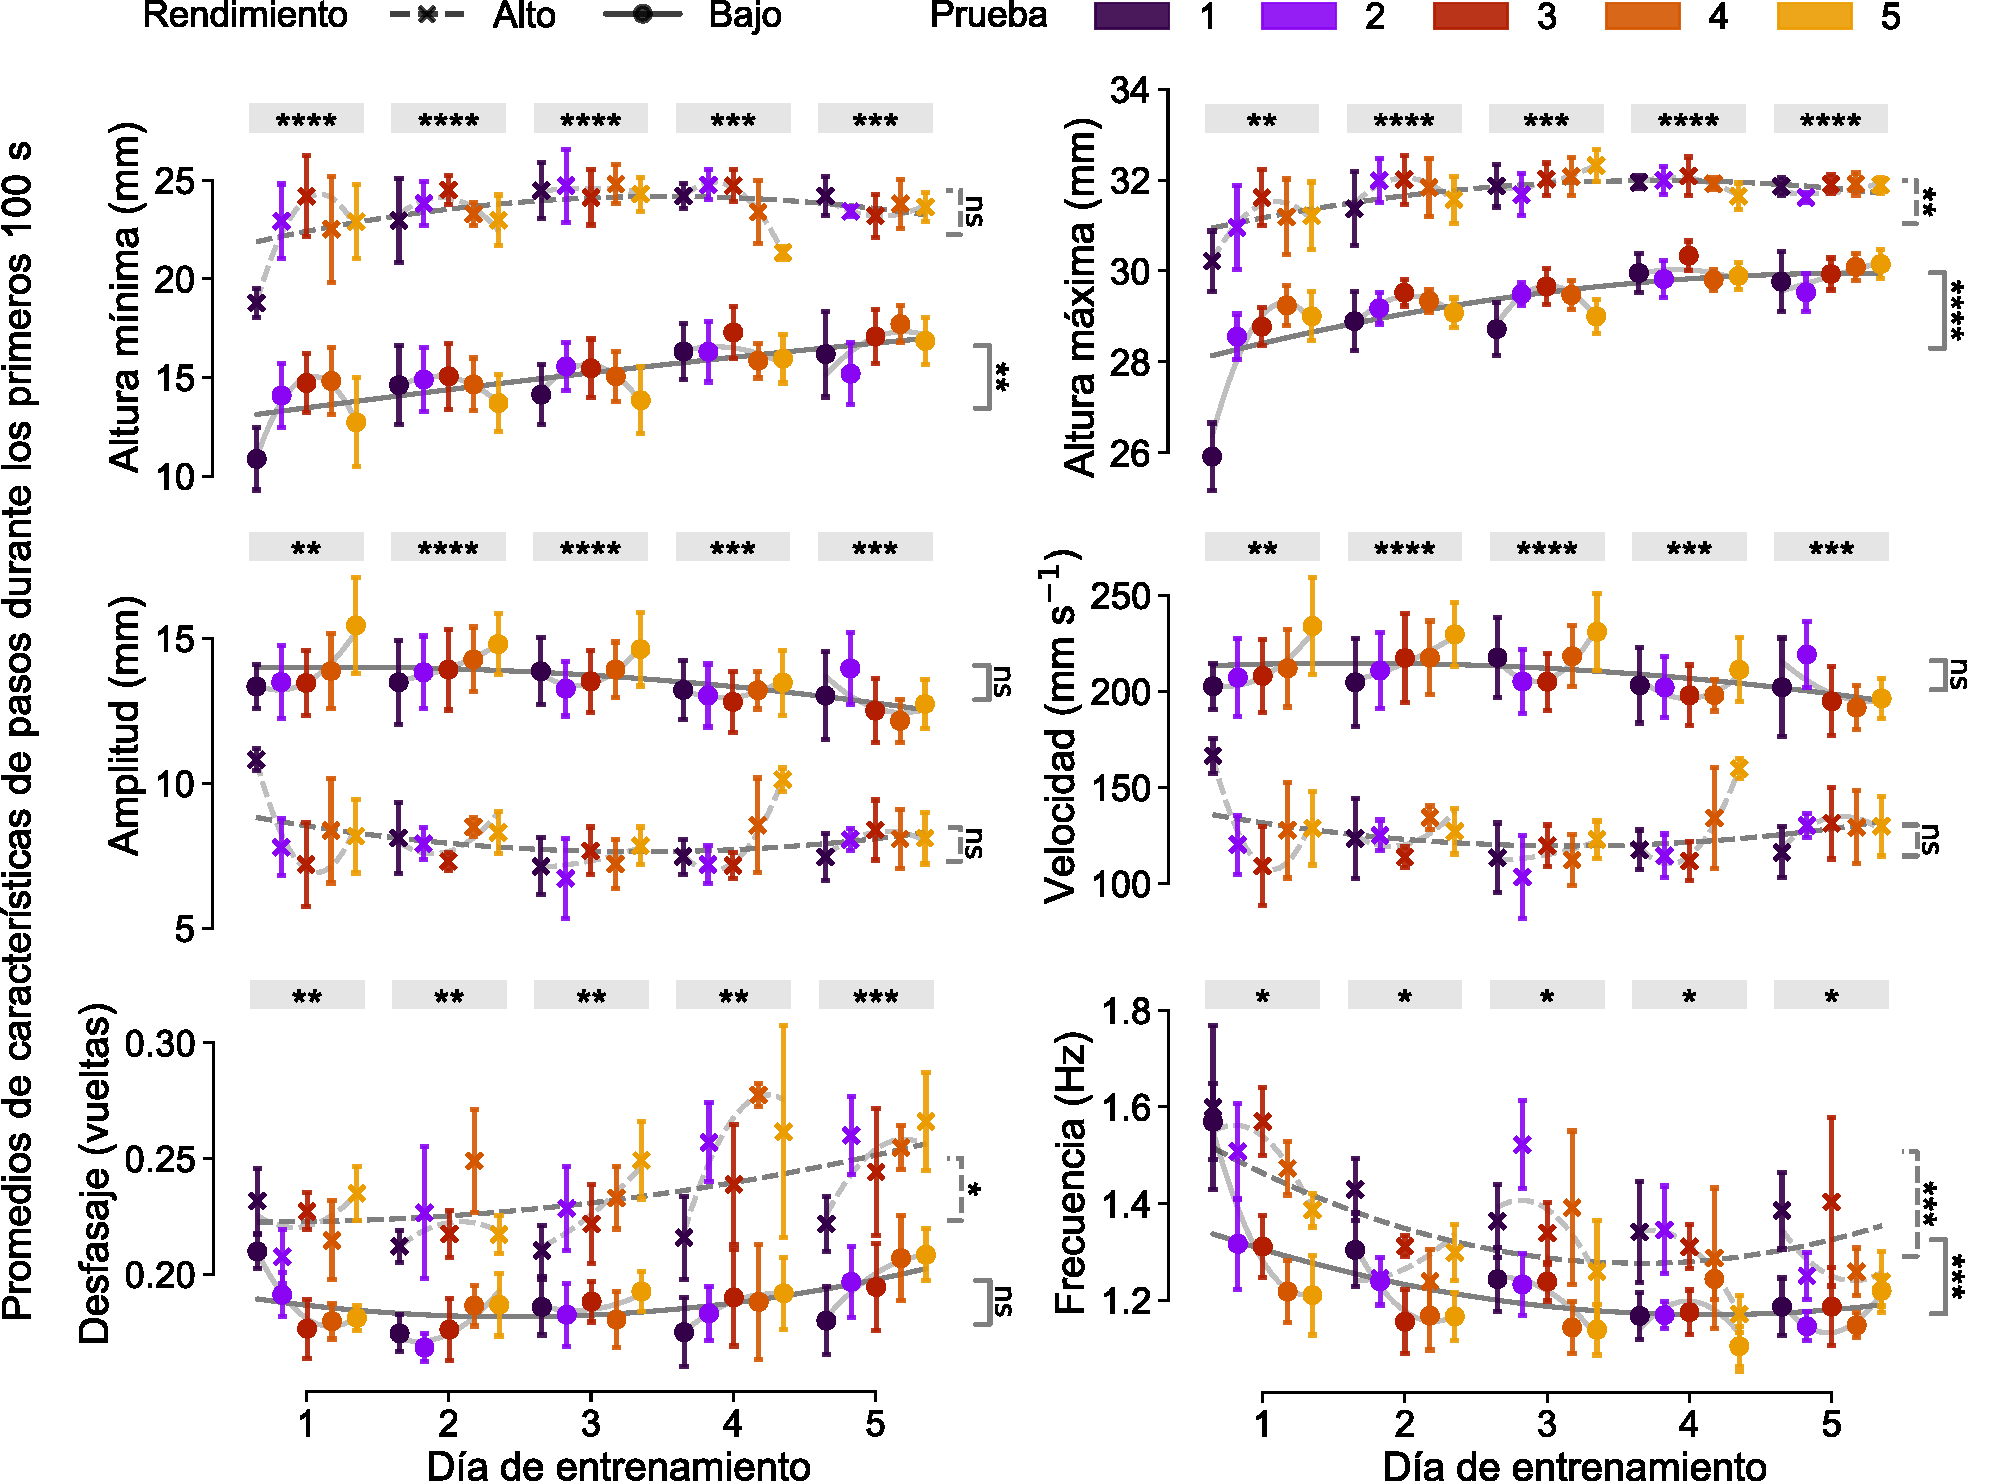
\includegraphics[width=0.99\linewidth]{figuras/capitulo3/metricas_promedio.pdf}
        \caption{\textbf{Promedio de las características de pasos durante los primeros 100 s de las pruebas rotarod.} Los puntos muestran el promedio por grupo de rendimiento y las barras son el error estándar del promedio.
            En cada subfigura, los rectángulos grises superiores indican los p-valores T-test entre grupos de rendimiento para cada día.
            Los corchetes en los márgenes derechos indican, para cada grupo de rendimiento, los p-valores \textit{one-way} ANOVA agrupando por día de entrenamiento.}
        \label{fig:capitulo3_metricas_promedio}
    \end{figure}

    \clearpage

    \section{Pendiente}\label{sec:apendice_pendiente}

    \begin{figure}[htbp]
        \centering
        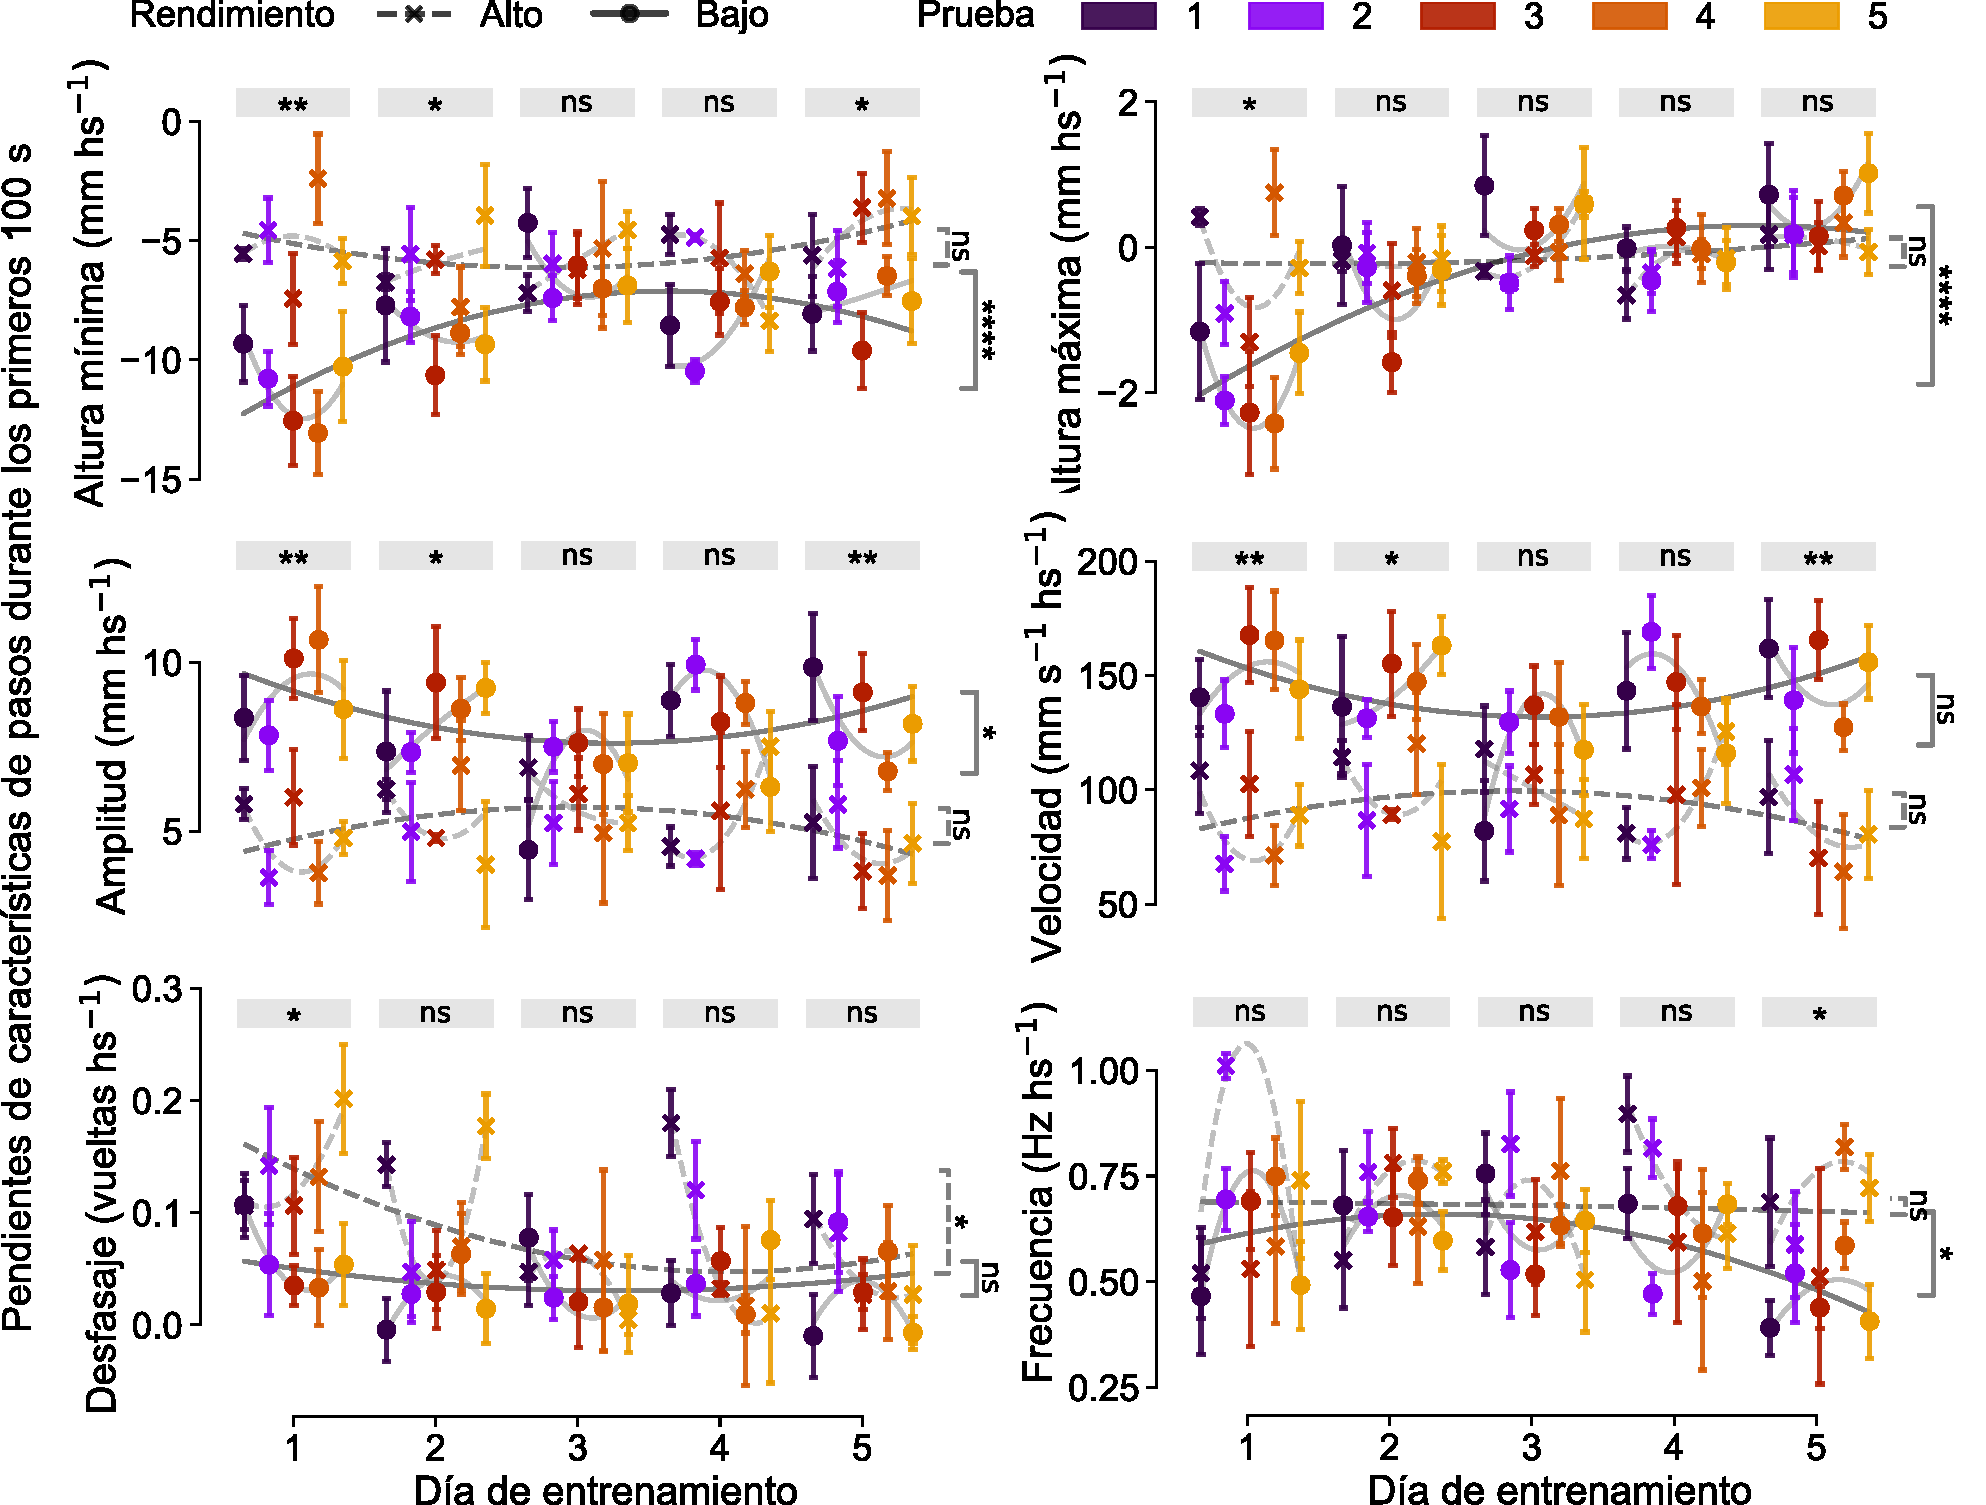
\includegraphics[width=0.99\linewidth]{figuras/capitulo3/metricas_pendiente.pdf}
        \caption{\textbf{Pendiente de las características de pasos durante los primeros 100 s de las pruebas rotarod.} Los puntos muestran el promedio por grupo de rendimiento y las barras son el error estándar del promedio.
            En cada subfigura, los rectángulos grises superiores indican los p-valores T-test entre grupos de rendimiento para cada día.
            Los corchetes en los márgenes derechos indican, para cada grupo de rendimiento, los p-valores \textit{one-way} ANOVA agrupando por día de entrenamiento.}
        \label{fig:capitulo3_metricas_pendiente}
    \end{figure}

    \clearpage

    \section{RMSE}\label{sec:apendice_rmse}

    \begin{figure}[htbp]
        \centering
        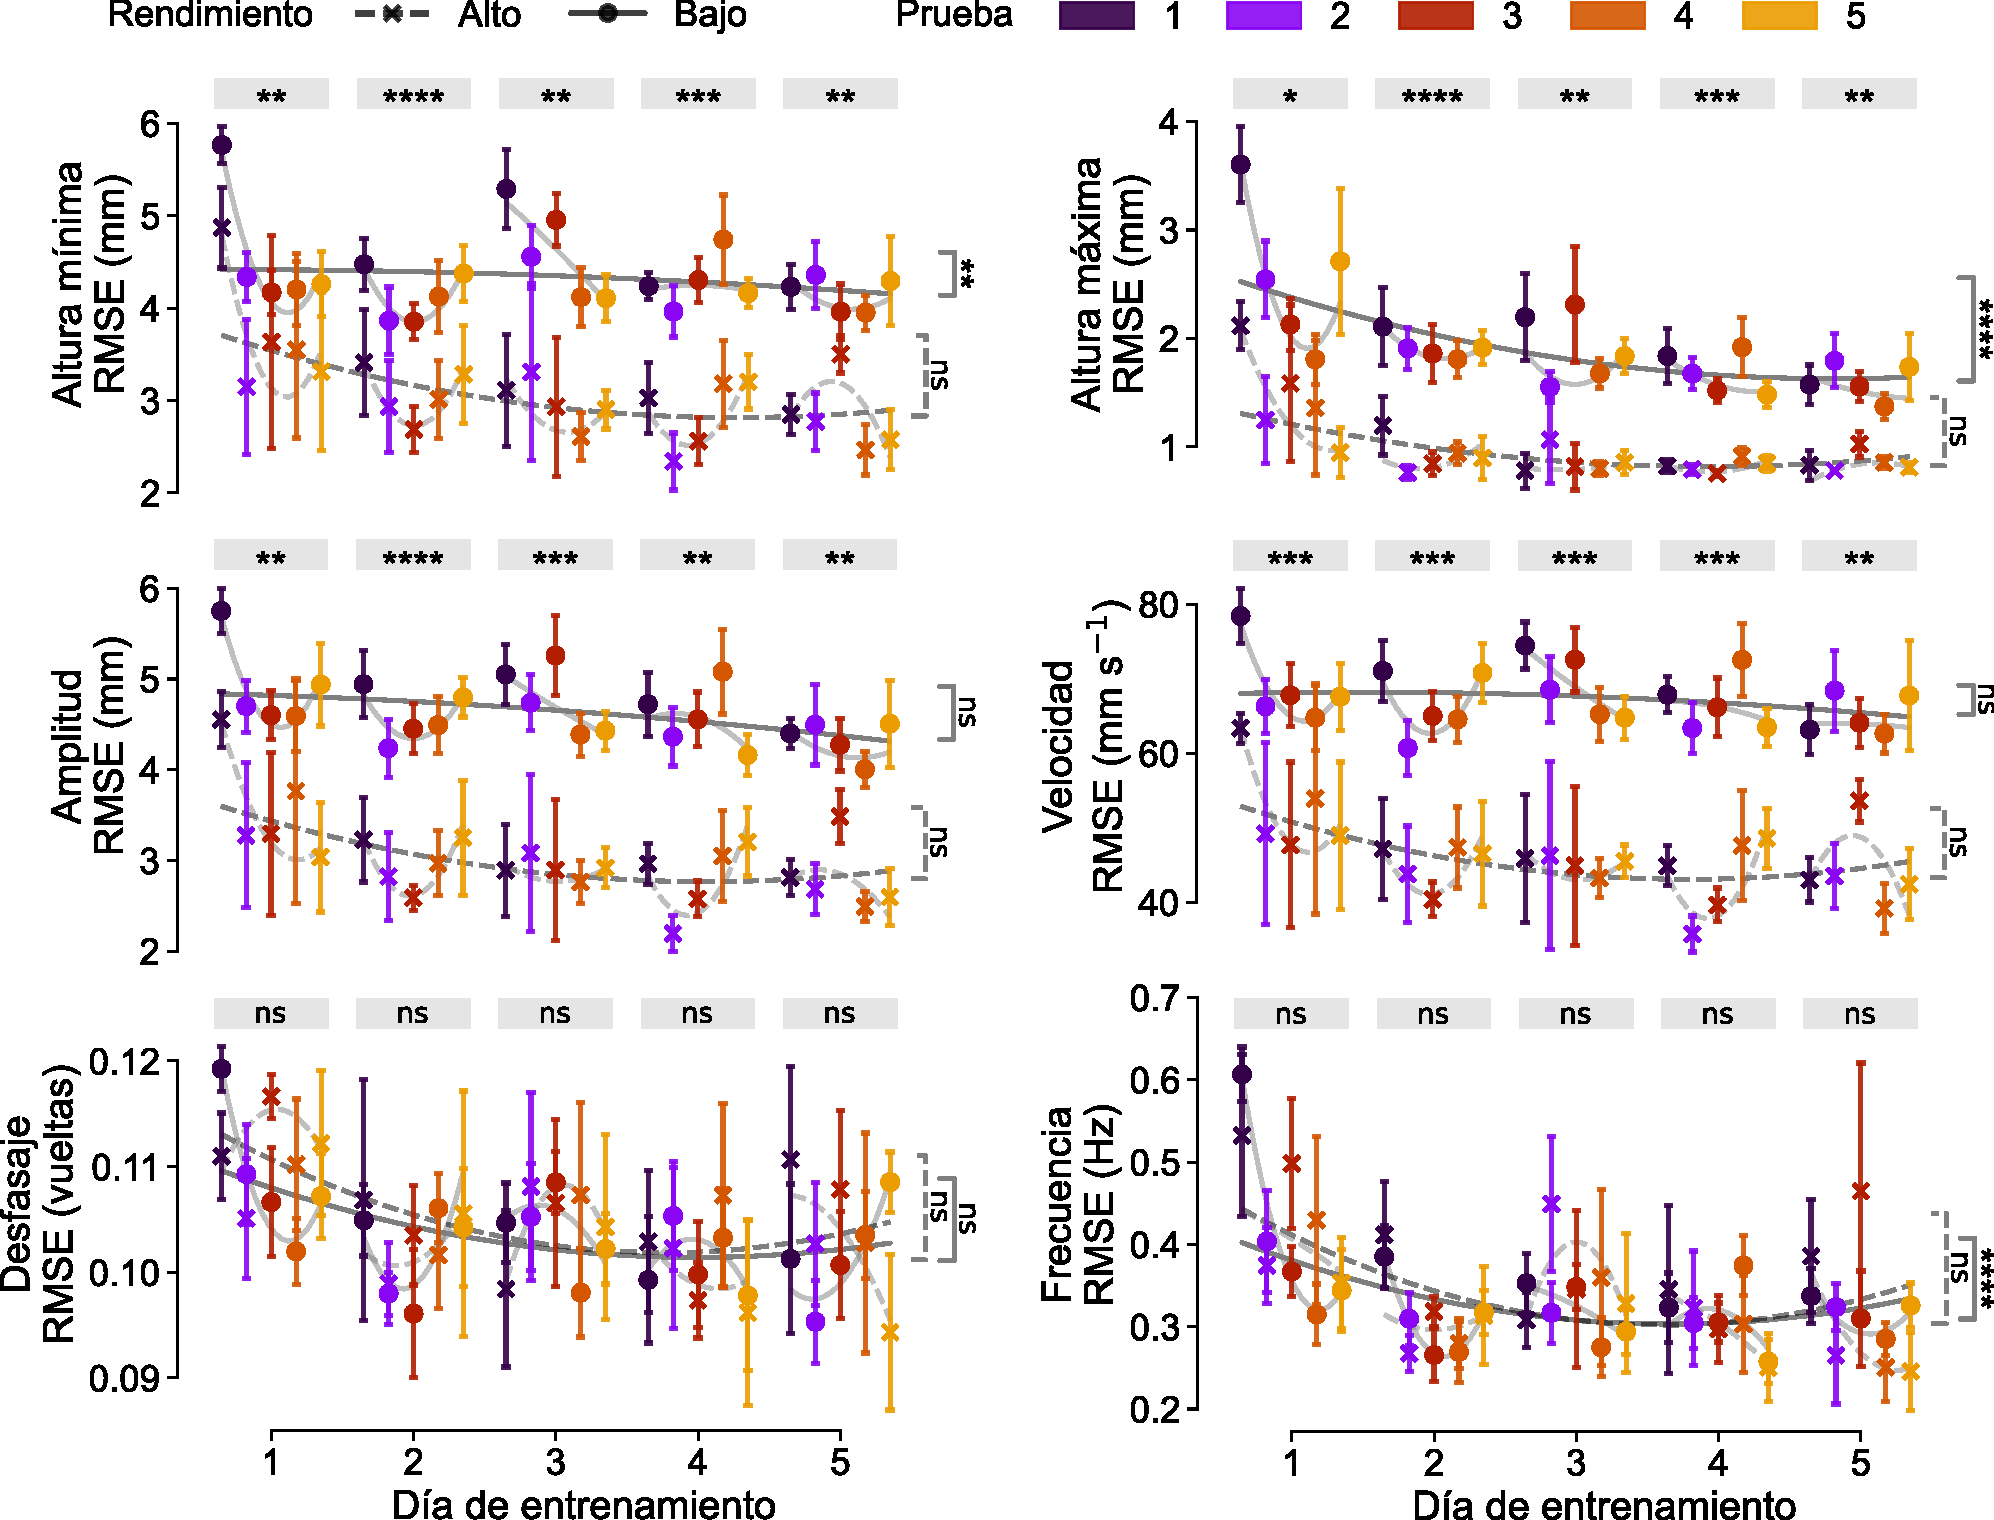
\includegraphics[width=0.99\linewidth]{figuras/capitulo3/metricas_rmse.pdf}
        \caption{\textbf{RMSE de las características de pasos durante los primeros 100 s de las pruebas rotarod.} Los puntos muestran el promedio por grupo de rendimiento y las barras son el error estándar del promedio.
            En cada subfigura, los rectángulos grises superiores indican los p-valores T-test entre grupos de rendimiento para cada día.
            Los corchetes en los márgenes derechos indican, para cada grupo de rendimiento, los p-valores \textit{one-way} ANOVA agrupando por día de entrenamiento.}
        \label{fig:capitulo3_metricas_rmse}
    \end{figure}

    \clearpage

    \chapter{Análisis de mapas de comportamiento}\label{cha:apendice_mapas}

    Figuras suplementarias sobre el análisis de las proyecciones UMAP y los \textit{labels} de comportamiento obtenidos a partir de los dos conjuntos de características: PCA de los espectros \textit{wavelet} y características de pasos y poses.

    \section{Caracterización de los mapas UMAP}\label{sec:apendice_umap}

    \begin{figure}[htbp]
        \centering
        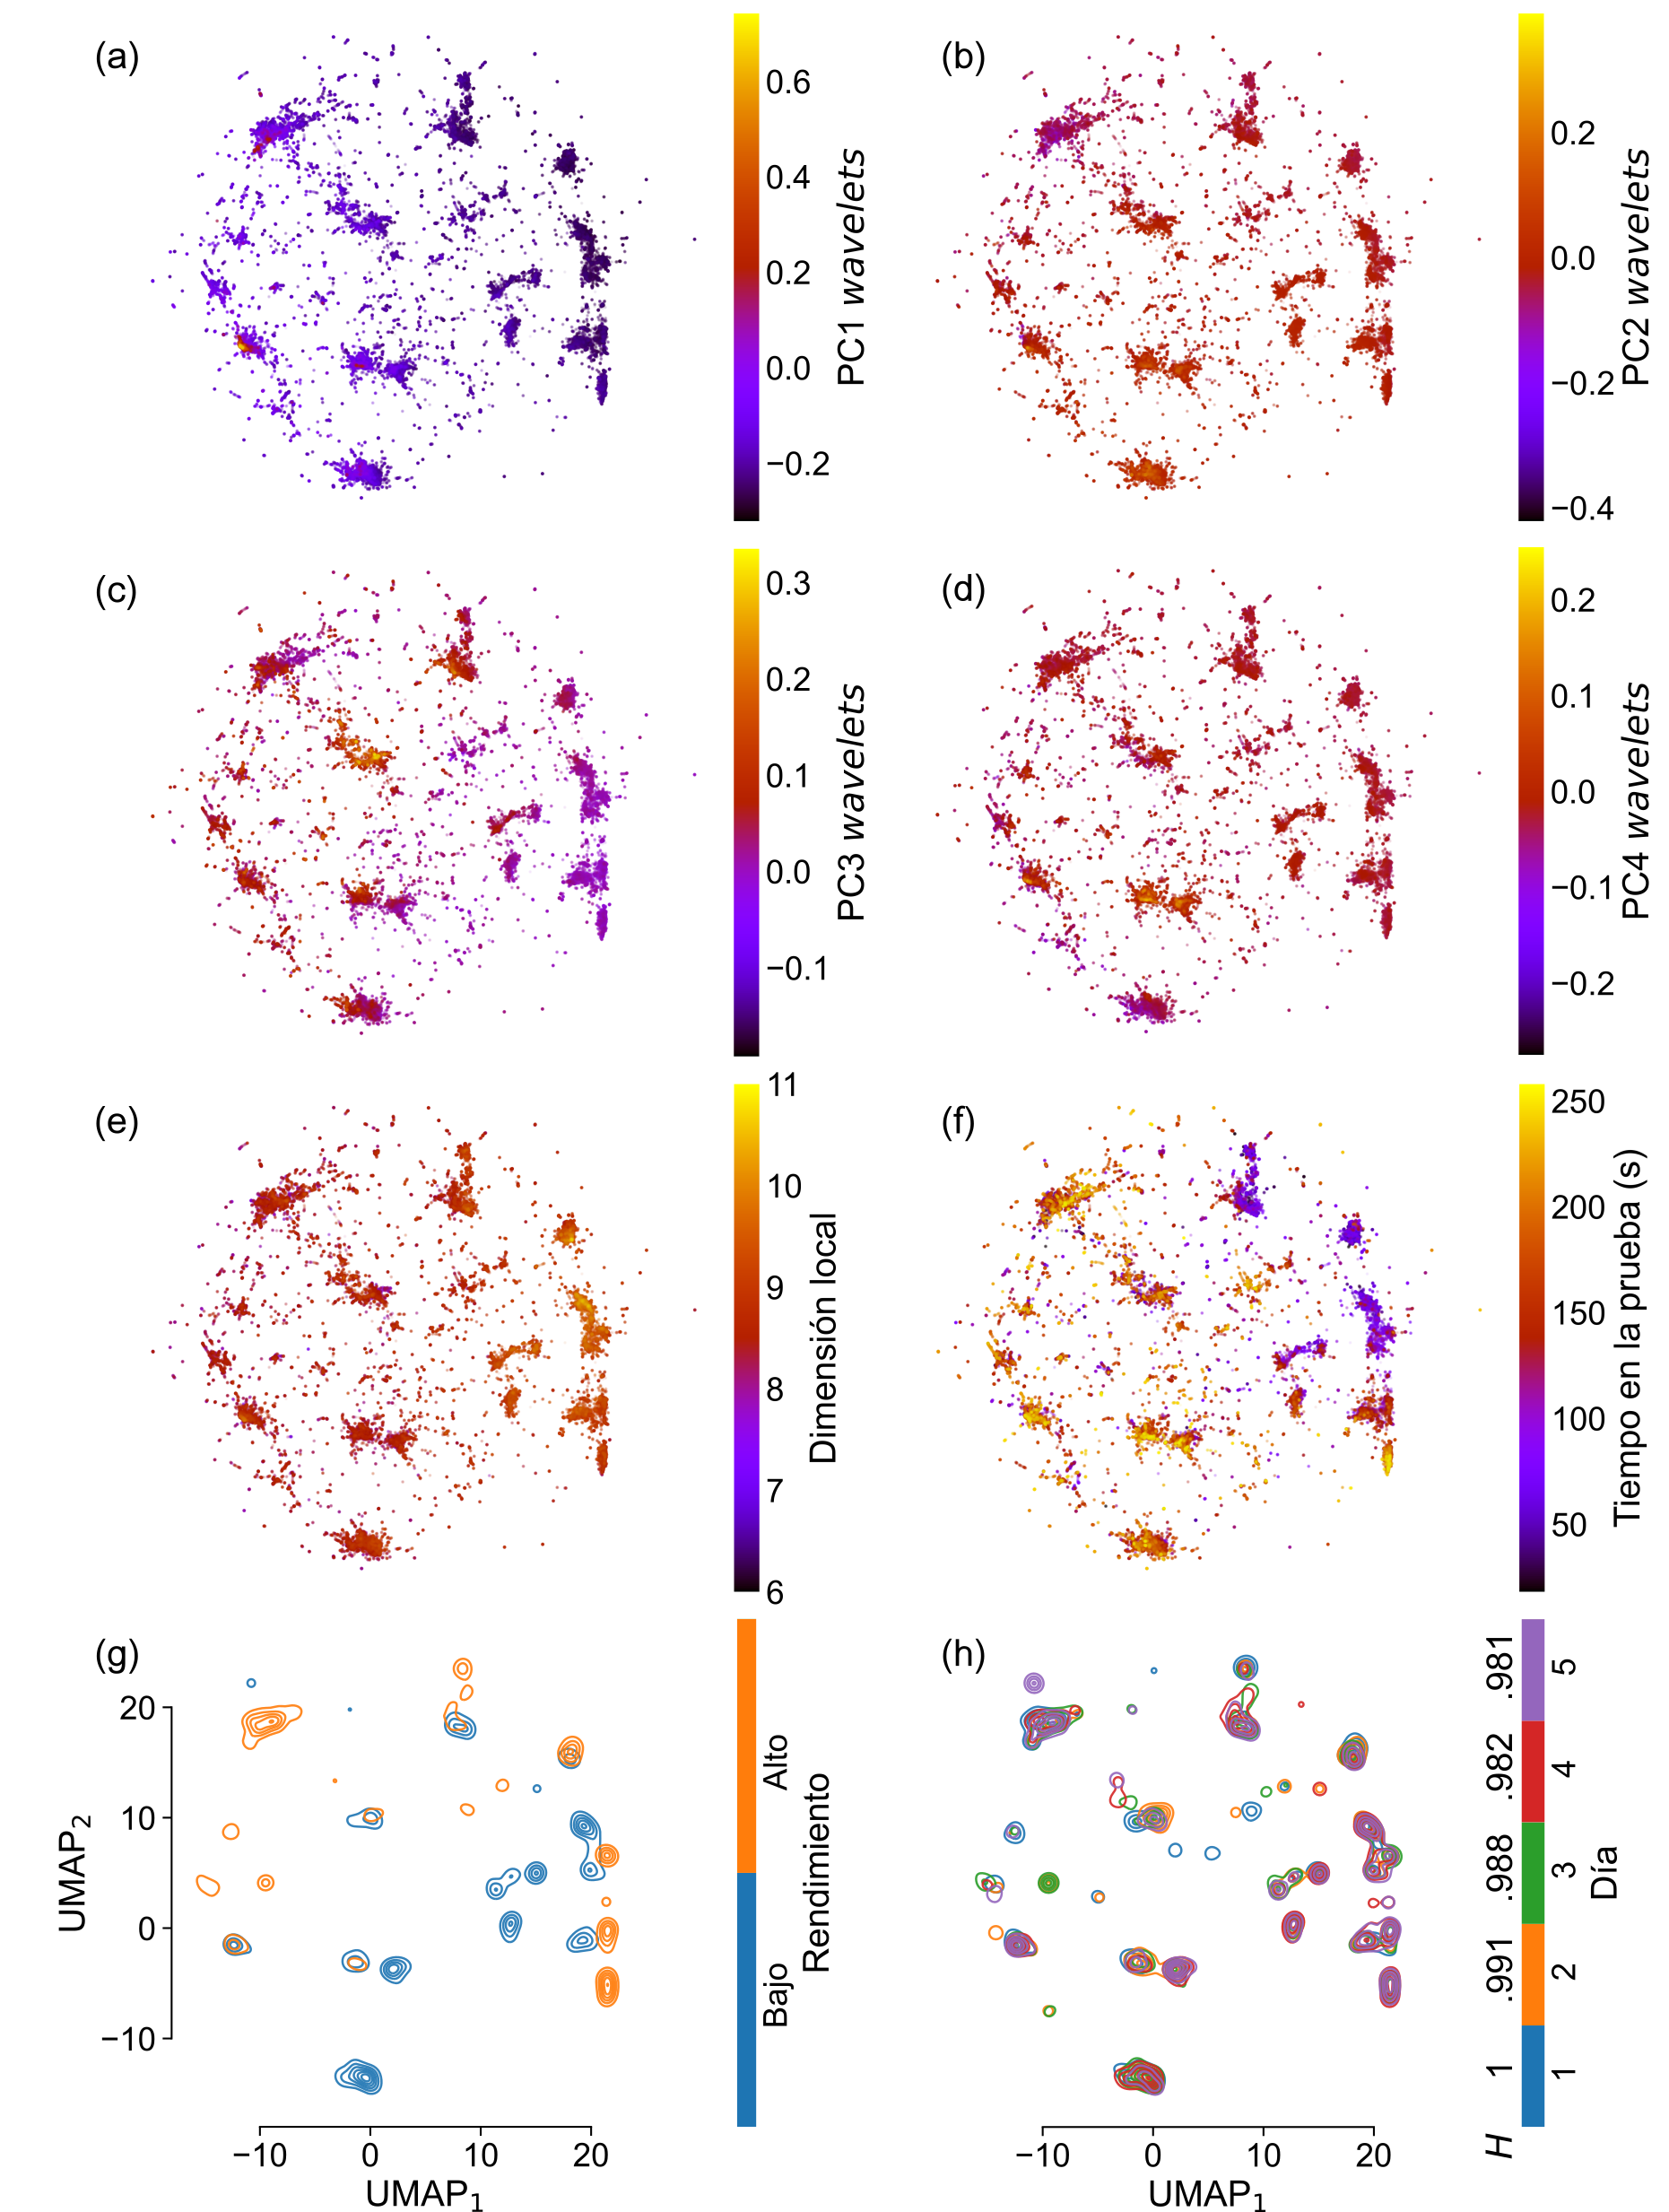
\includegraphics[width=0.9\linewidth]{figuras/capitulo4/umap_wav.png}
        \caption{\textbf{UMAP de las componentes principales de los espectros \textit{wavelet}.} Valores de las primeras cuatro componentes principales (PCs): (a) PC1, (b) PC2, (c) PC3 y (d) PC4. (e) Dimensión local del mapa. La dimensión local es el número de componentes PCA que explican el 80\% de la varianza en el subconjunto de datos formado por los vecinos más cercanos de cada punto en el mapa. (f) Tiempo transcurrido en cada prueba rotarod. (g) Densidad de probabilidad  en el espacio UMAP, condicionada por grupo de rendimiento. (h) Densidad de probabilida condicionada por día de entrenamiento. La entropía $H$ de las distribuciones disminuye con los días de entrenamiento, tomando como valor de referencia a la entropía del día 1.}
        \label{fig:capitulo4_umap_wav}
    \end{figure}

    \begin{figure}[htbp]
        \centering
        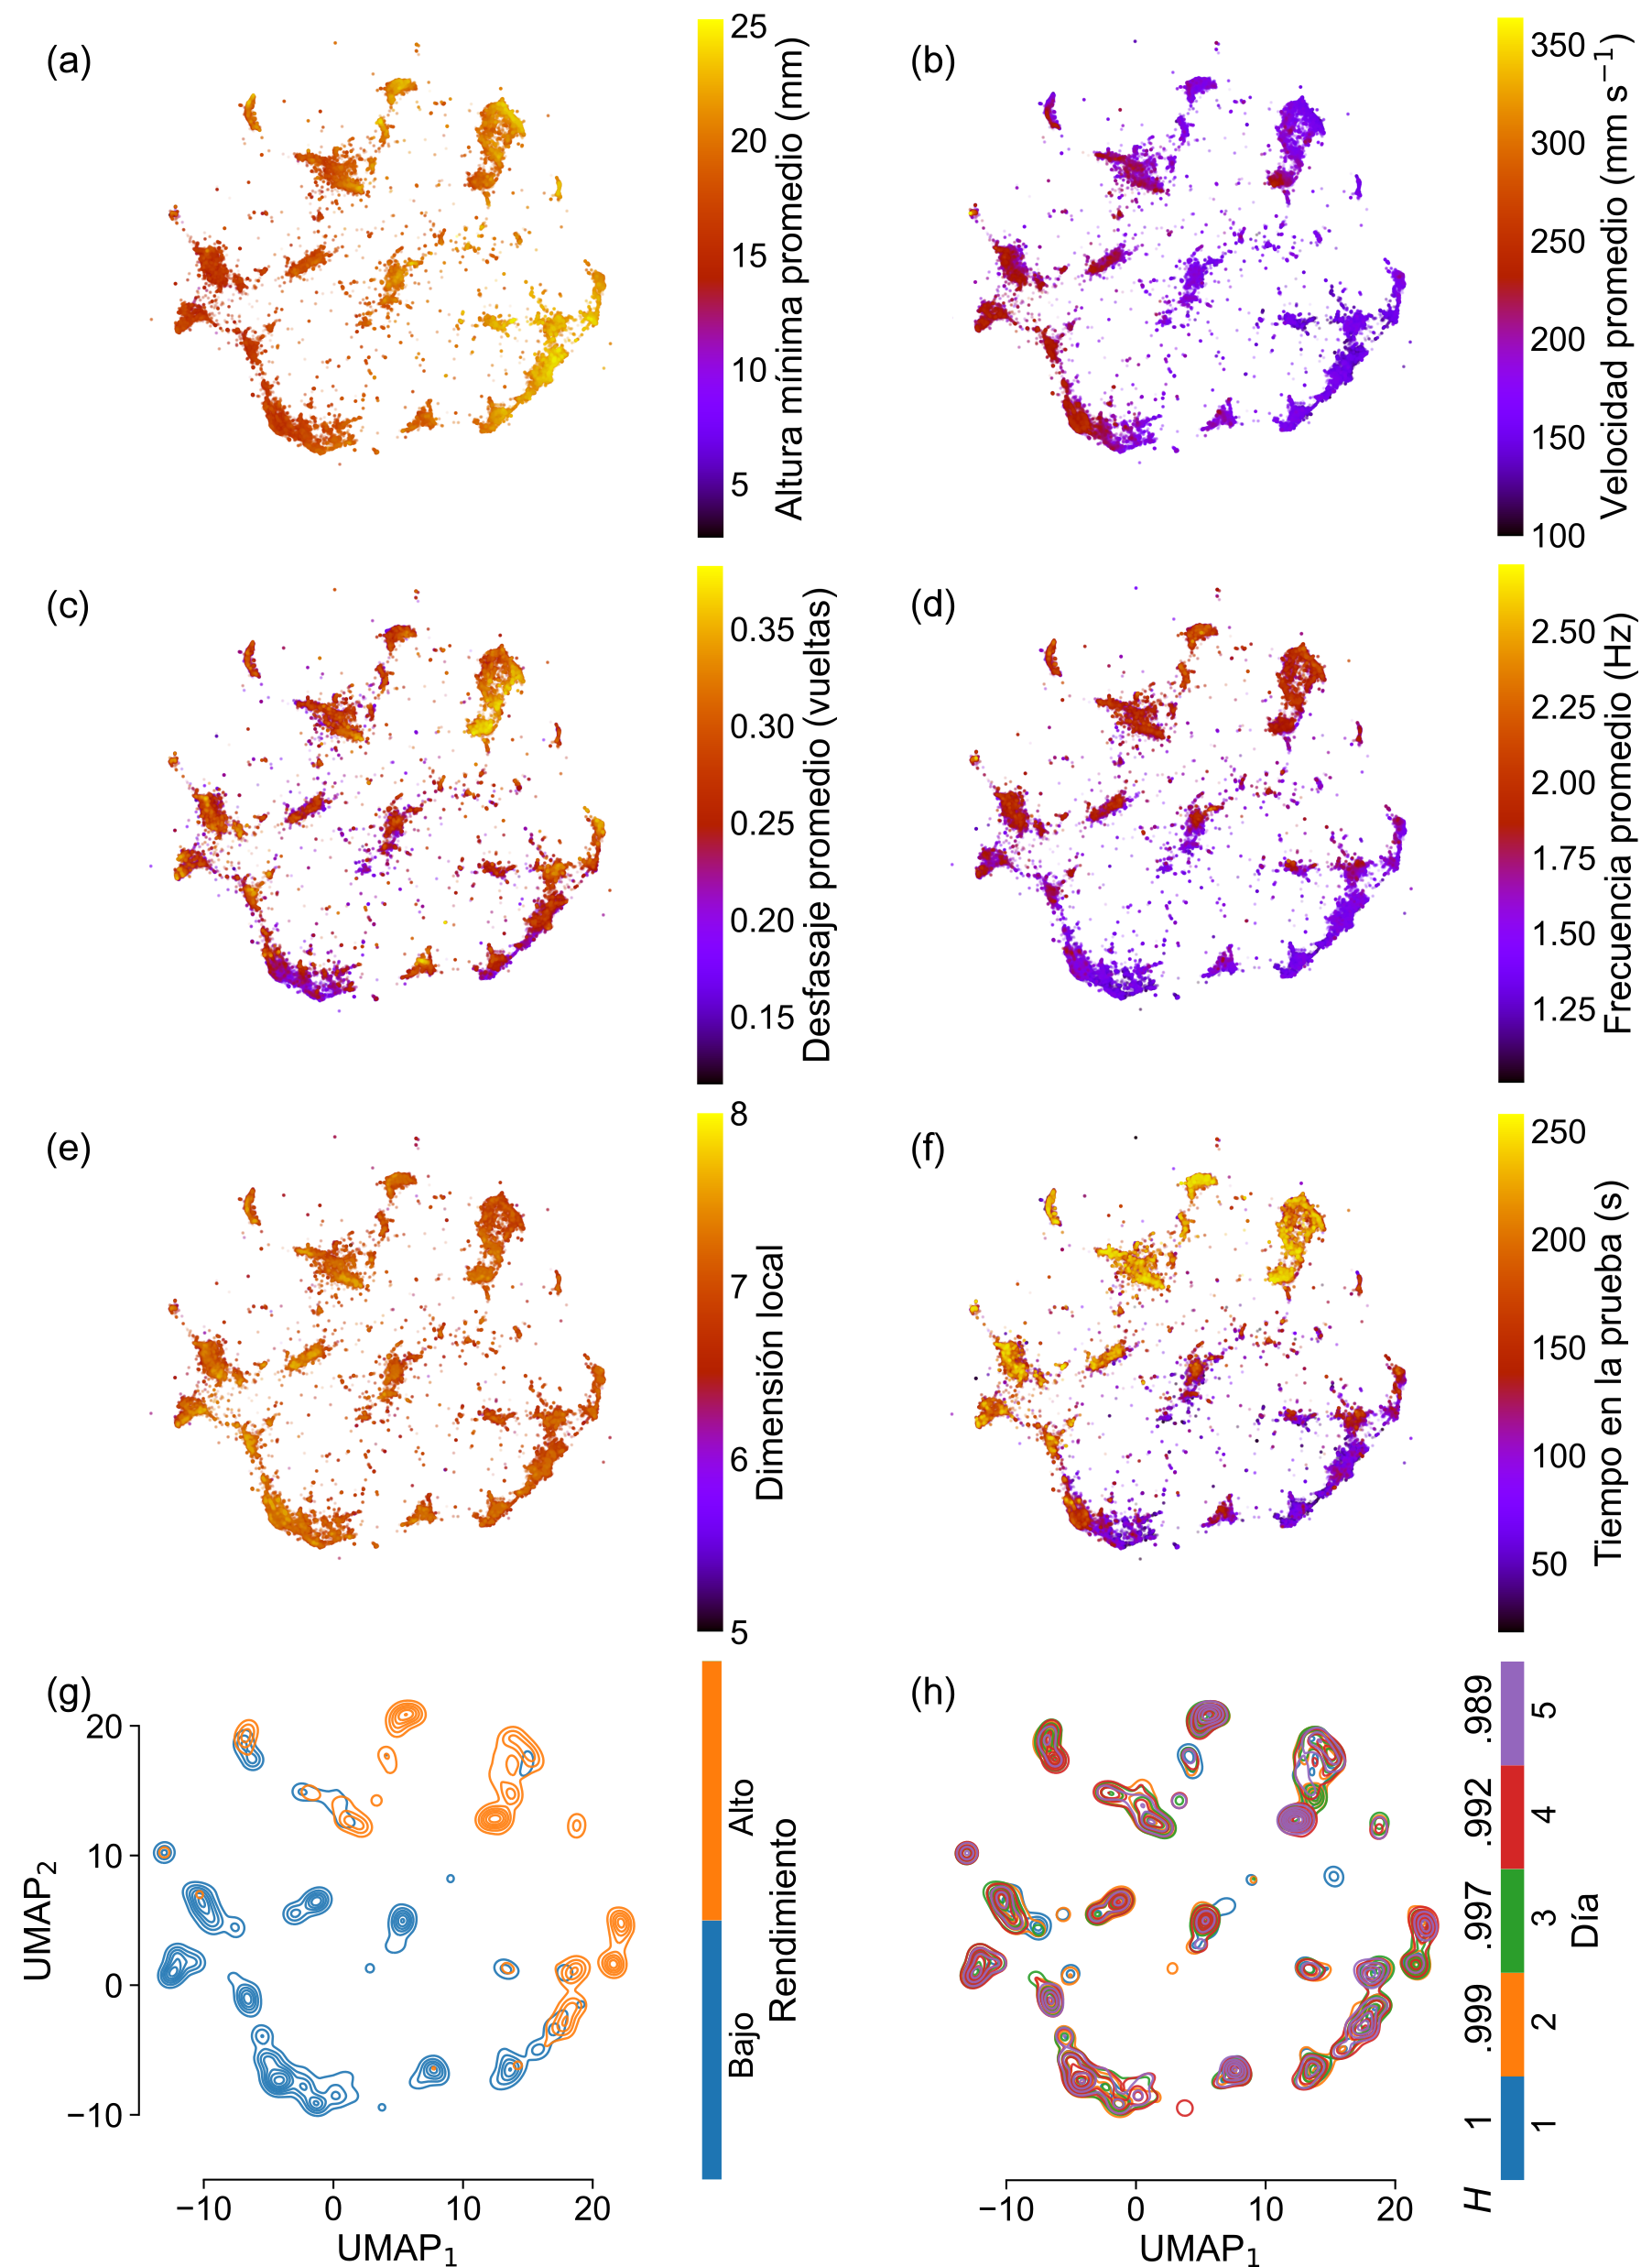
\includegraphics[width=0.9\linewidth]{figuras/capitulo4/umap_stp.png}
        \caption{\textbf{UMAP de las características de pasos y poses.} Valores promedio de algunas características de pasos: (a) altura mínima, (b) velocidad, (c) desfasaje y (d) frecuencia. (e) Dimensión local del mapa. La dimensión local es el número de componentes PCA que explican el 80\% de la varianza en el subconjunto de datos formado por los vecinos más cercanos de cada punto en el mapa. (f) Tiempo transcurrido en cada prueba rotarod. (g) Densidad de probabilidad  en el espacio UMAP, condicionada por grupo de rendimiento. (h) Densidad de probabilida condicionada por día de entrenamiento. La entropía $H$ de las distribuciones disminuye con los días de entrenamiento, tomando como valor de referencia a la entropía del día 1.}
        \label{fig:capitulo4_umap_stp}
    \end{figure}

    \clearpage

    \section{\textit{Labels} de comportamiento}\label{sec:apendice_labels}

    \begin{figure}[htbp]
        \centering
        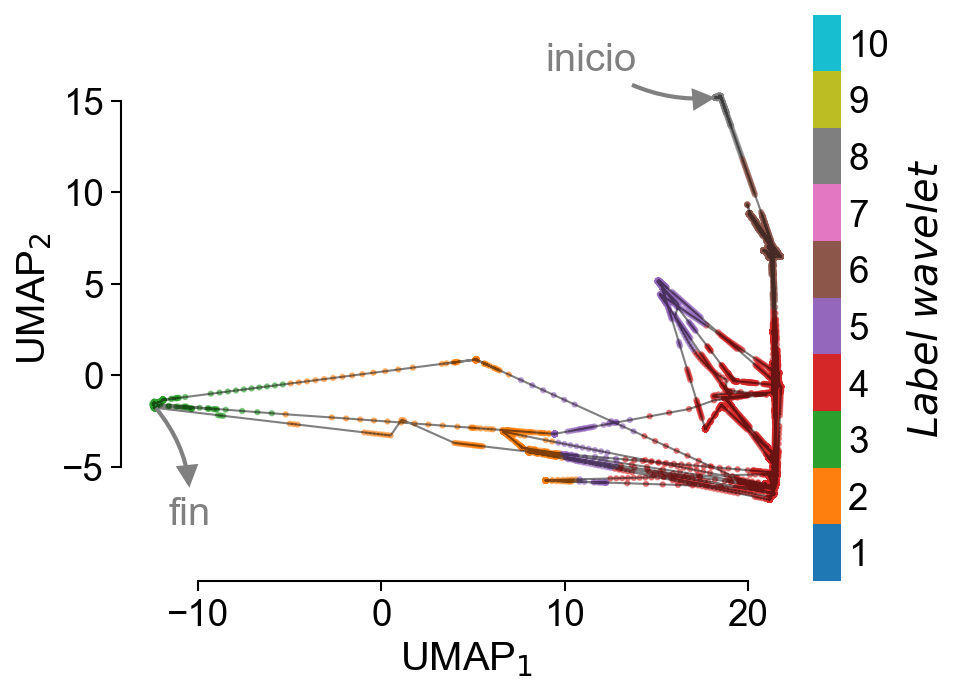
\includegraphics[width=0.7\linewidth]{figuras/capitulo4/label_serie_mapa_wav.png}
        \caption{\textbf{\textit{Labels} de comportamiento en el mapa UMAP \textit{wavelet}.}
            Serie temporal de \textit{labels}, vistos en el mapa UMAP \textit{wavelet}, durante la ejecución de una prueba rotarod (ídem \autoref{fig:capitulo2_posiciones})}
        \label{fig:capitulo4_label_serie_mapa_wav}
    \end{figure}

    \begin{figure}[htbp]
        \centering
        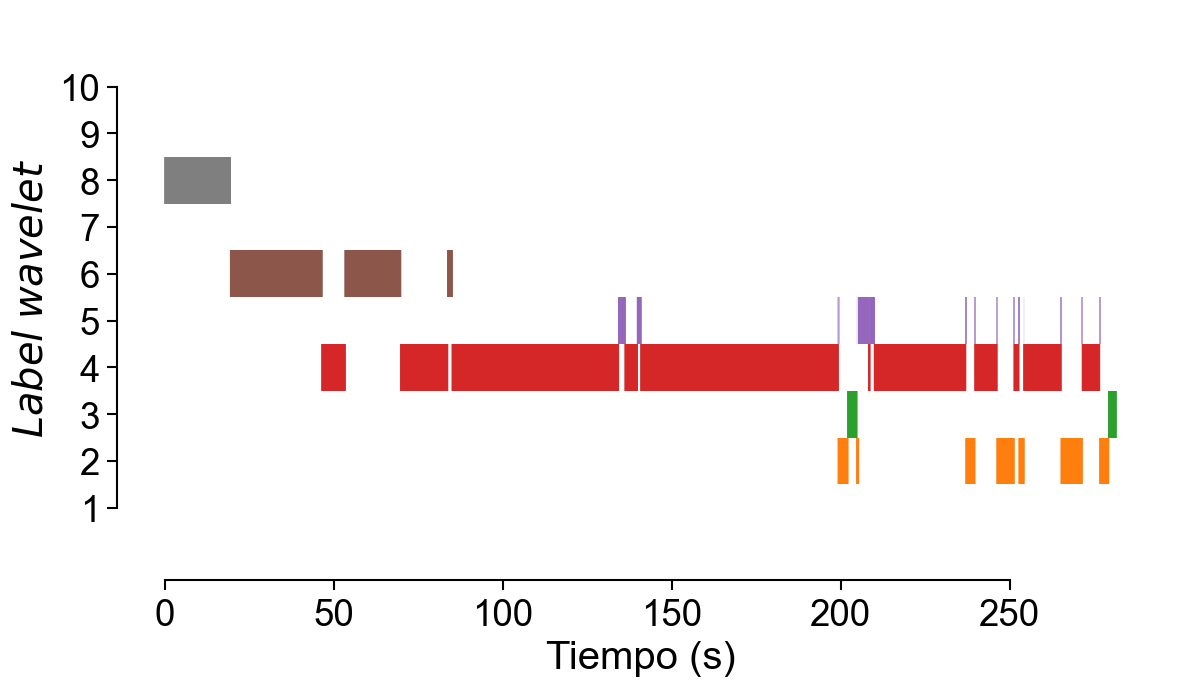
\includegraphics[width=0.7\linewidth]{figuras/capitulo4/label_secuencia_wav.png}
        \caption{\textbf{Secuencia de \textit{labels} \textit{wavelet}.}
            Secuencia de \textit{labels wavelet} durante la ejecución de una prueba rotarod (ídem \autoref{fig:capitulo2_posiciones})}
        \label{fig:capitulo4_label_secuencia_wav}
    \end{figure}

    \begin{figure}[htbp]
        \centering
        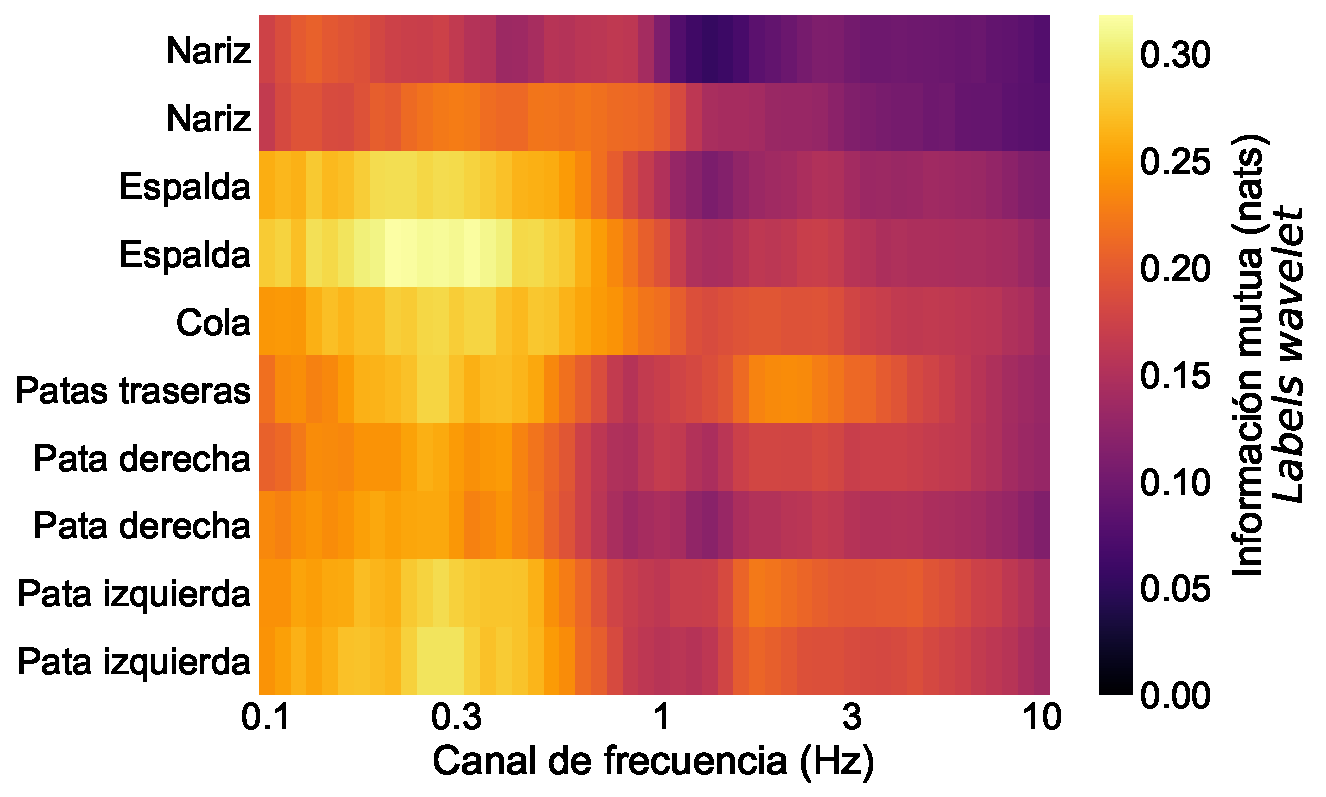
\includegraphics[width=0.7\linewidth]{figuras/capitulo4/mi_labels_wav.pdf}
        \caption{\textbf{Información mutua entre los \textit{labels} \textit{wavelets} y los espectros \textit{wavelet}.}}
        \label{fig:capitulo4_mi_labels_wav}
    \end{figure}

    \begin{figure}[htbp]
        \centering
        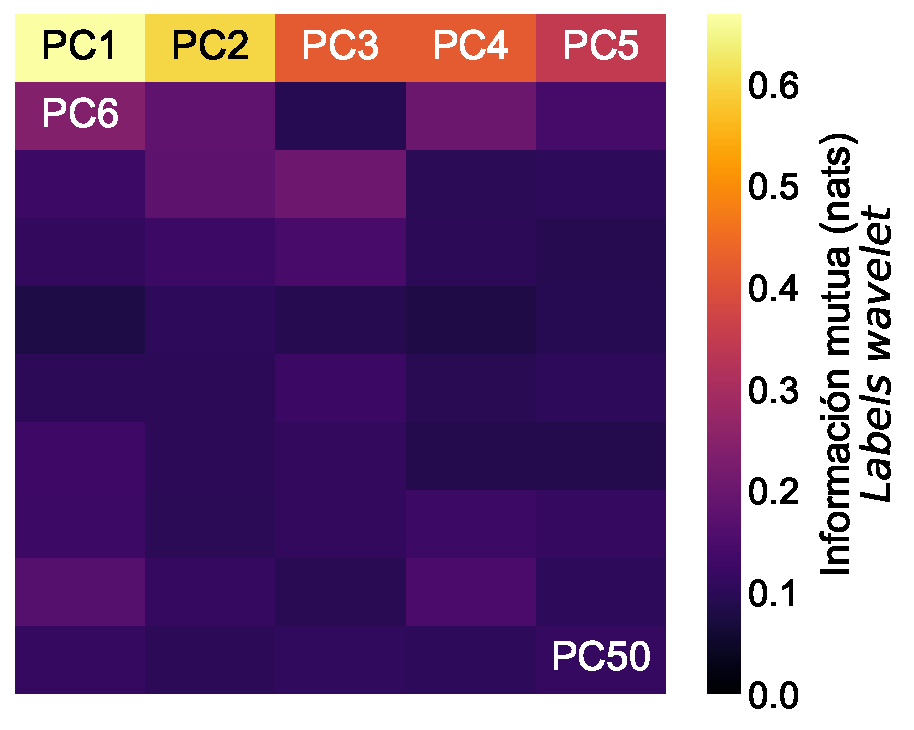
\includegraphics[width=0.7\linewidth]{figuras/capitulo4/mi_labels_pca.pdf}
        \caption{\textbf{Información mutua entre los \textit{labels} \textit{wavelets} y el PCA de los espectros \textit{wavelet}.}}
        \label{fig:capitulo4_mi_labels_pca}
    \end{figure}

    \begin{figure}[htbp]
        \centering
        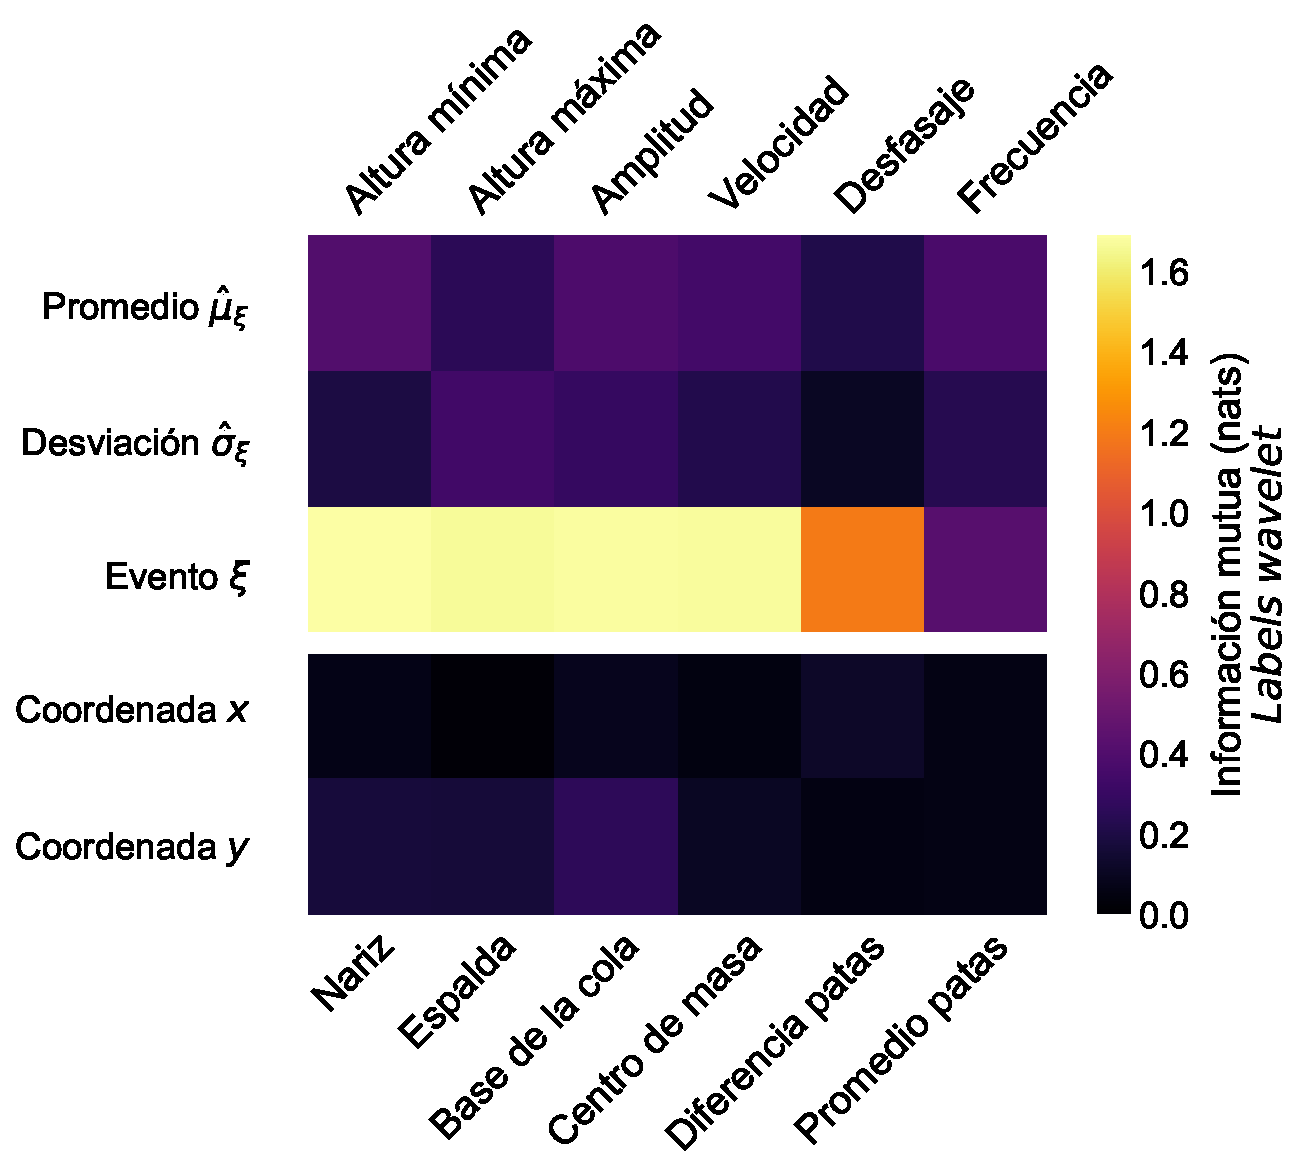
\includegraphics[width=0.7\linewidth]{figuras/capitulo4/mi_contra_labels_scaler_stp.pdf}
        \caption{\textbf{Información mutua entre los \textit{labels} \textit{wavelets} y las características de pasos y poses.}}
        \label{fig:capitulo4_mi_contra_labels_scaler_stp}
    \end{figure}

    \begin{figure}[htbp]
        \centering
        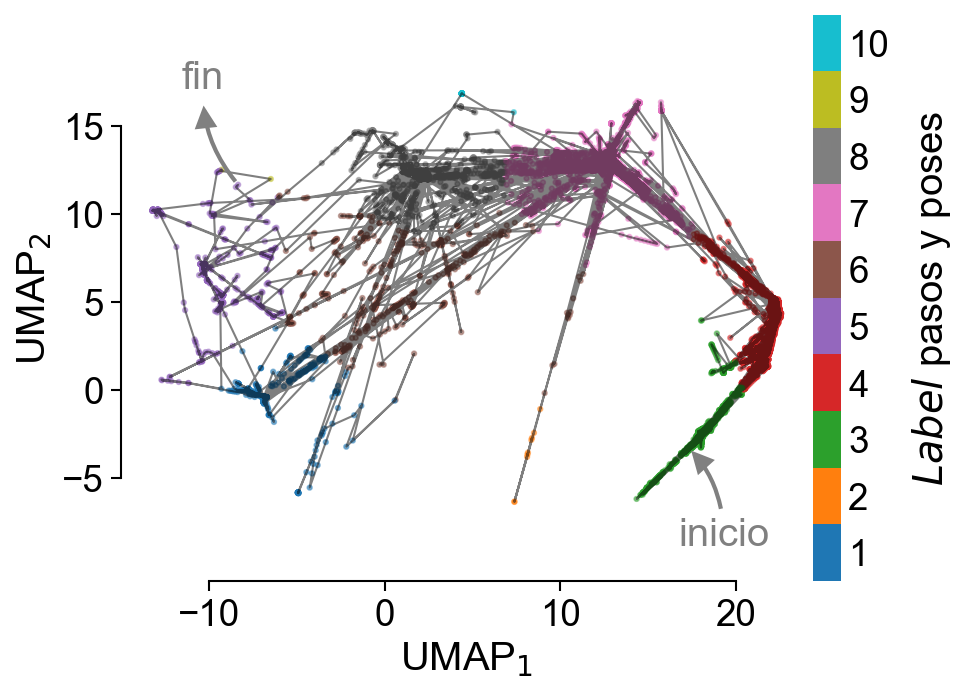
\includegraphics[width=0.7\linewidth]{figuras/capitulo4/label_serie_mapa_stp.png}
        \caption{\textbf{\textit{Labels} de comportamiento en el mapa UMAP de pasos y poses.}
            Serie temporal de \textit{labels}, vistos en el mapa UMAP de pasos y poses, durante la ejecución de una prueba rotarod (ídem \autoref{fig:capitulo2_posiciones})}
        \label{fig:capitulo4_label_serie_mapa_stp}
    \end{figure}

    \begin{figure}[htbp]
        \centering
        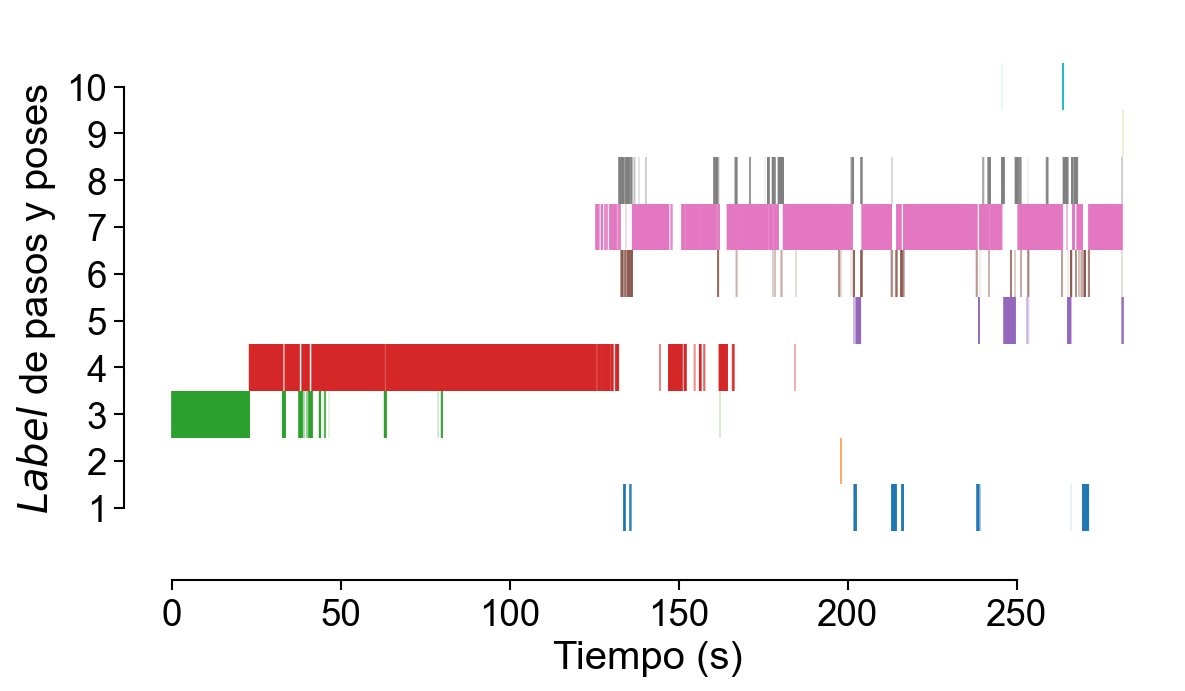
\includegraphics[width=0.7\linewidth]{figuras/capitulo4/label_secuencia_stp.png}
        \caption{\textbf{Secuencia de \textit{labels} de pasos y poses.}
            Secuencia de \textit{labels} de pasos y poses durante la ejecución de una prueba rotarod (ídem \autoref{fig:capitulo2_posiciones})}
        \label{fig:capitulo4_label_secuencia_stp}
    \end{figure}

    \begin{figure}[htbp]
        \centering
        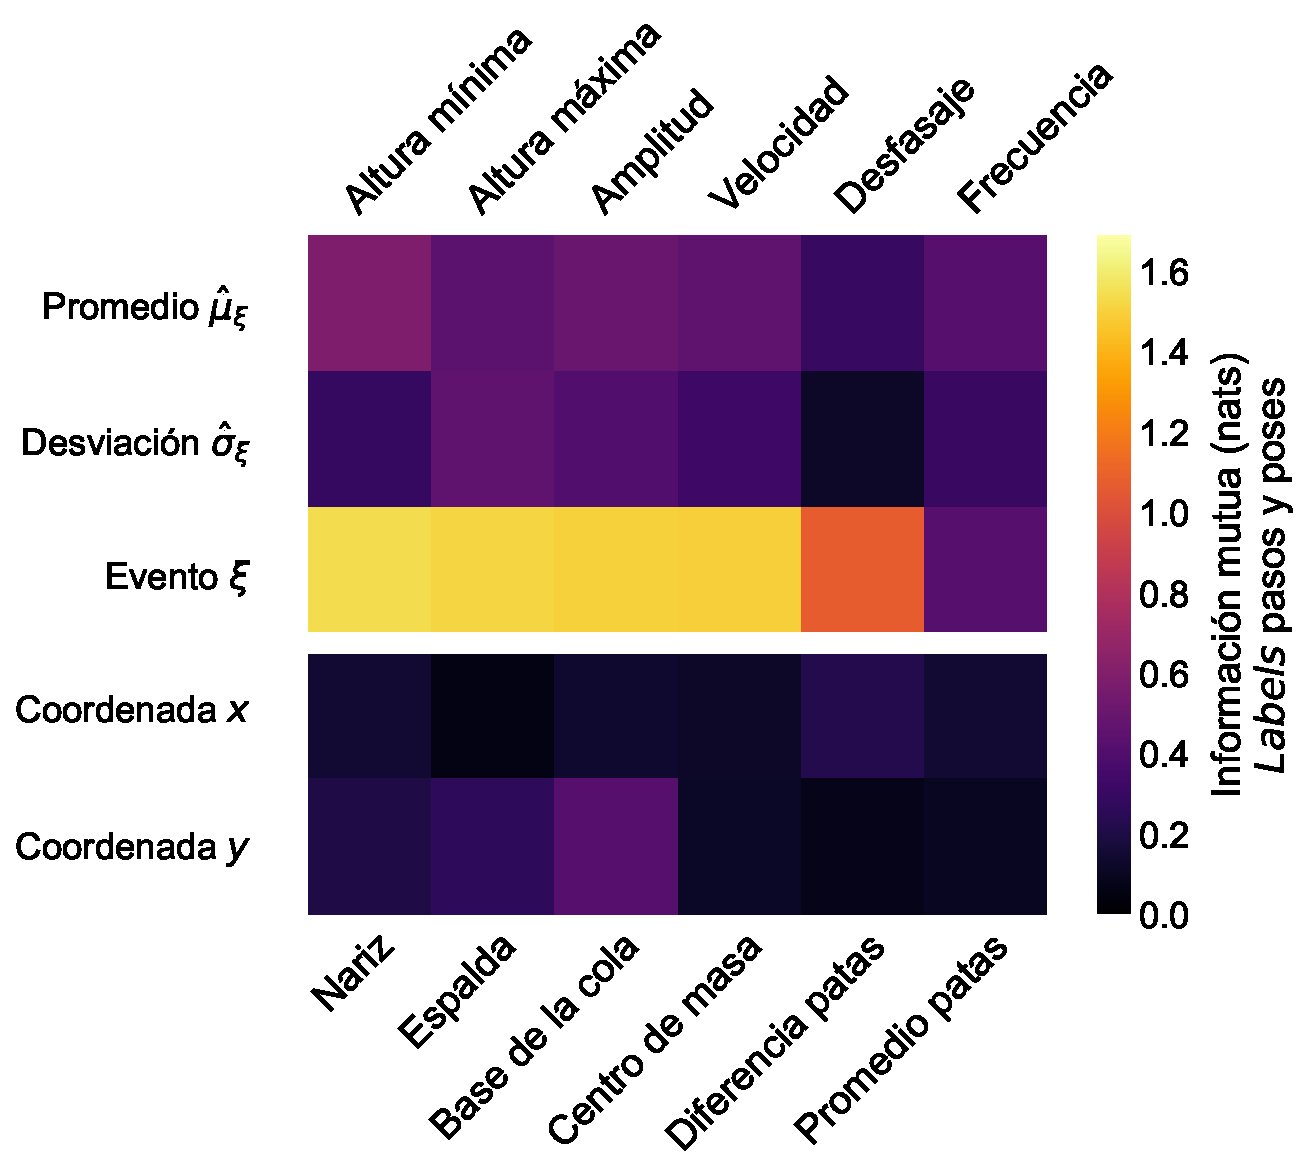
\includegraphics[width=0.7\linewidth]{figuras/capitulo4/mi_labels_scaler_stp.pdf}
        \caption{\textbf{Información mutua entre los \textit{labels} pasos y poses y las características de pasos y poses.}}
        \label{fig:capitulo4_mi_labels_scaler_stp}
    \end{figure}

    \begin{figure}[htbp]
        \centering
        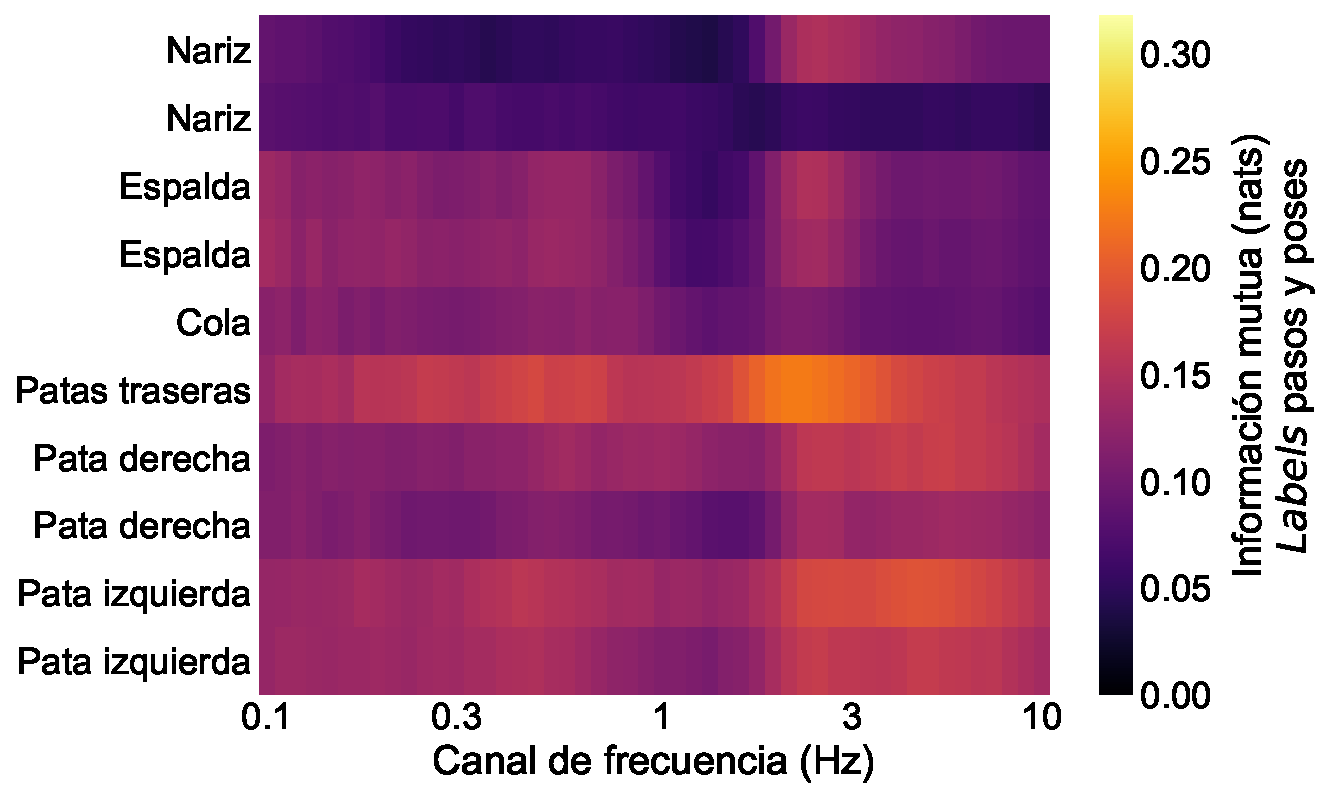
\includegraphics[width=0.7\linewidth]{figuras/capitulo4/mi_contra_labels_wav.pdf}
        \caption{\textbf{Información mutua entre los \textit{labels} pasos y poses y los espectros \textit{wavelet}.}}
        \label{fig:capitulo4_mi_contra_labels_wav}
    \end{figure}

    \begin{figure}[htbp]
        \centering
        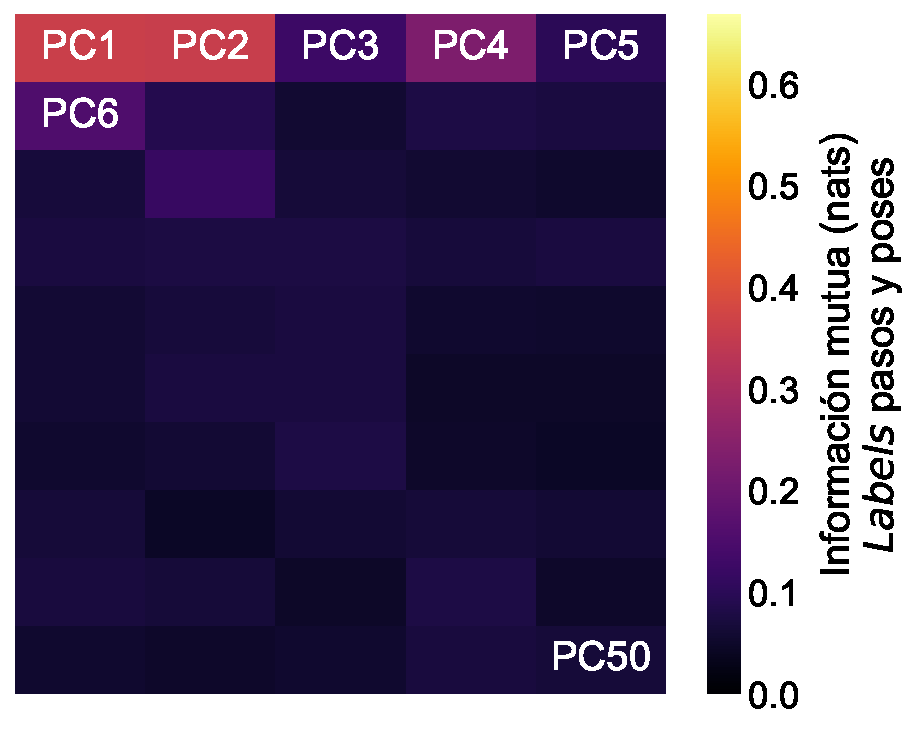
\includegraphics[width=0.7\linewidth]{figuras/capitulo4/mi_contra_labels_pca.pdf}
        \caption{\textbf{Información mutua entre los \textit{labels} pasos y poses y el PCA de los espectros \textit{wavelet}.}}
        \label{fig:capitulo4_mi_contra_labels_pca}
    \end{figure}

\end{appendix}
\listoffigures
\addcontentsline{toc}{chapter}{\listfigurename}
\listoftables
\addcontentsline{toc}{chapter}{\listtablename}

\end{document}